%initialising document, adjust papersize, fontsize and page orientation to your needs
\documentclass[a4paper, fontsize = 8pt, landscape]{scrartcl}
\usepackage{../../../misc_files/LateX/layout_and_colours}
\makeatletter
\def\input@path{{content/summary/}{content/examples/}}
\makeatother
\graphicspath{{content/}{content/summary/}{content/examples/}}

\title{Computertechnik}
\author{Jil Zerndt, Lucien Perret}
\date{January 2025}

\createtitlepagestyle
\createmainpagestyle
\begin{document}
\begin{multicols}{3}
	\thispagestyle{TitlePageStyle}
	\maketitle
	\sffamily
	
	\section{Computer Engineering}

\begin{concept}{Computer Engineering}
is where microelectronics and software meet:
\begin{itemize}
  \item Architecture and organization of computer systems
  \item Combines hardware and software to implement a computer
  \item Applications in embedded systems, information technology, and technical/scientific tools
  \item Historical development spanning over 70 years:
    \begin{itemize}
      \item 1940s: Relay/vacuum tubes
      \item 1950s: Transistors
      \item 1970s: Integrated circuits (CMOS)
      \item Present: Complex microprocessors with billions of transistors
    \end{itemize}
\end{itemize}
\end{concept}

\begin{theorem}{von Neumann Architecture}\\
The fundamental architecture used in most computers:
\begin{itemize}
  \item Single memory for both data and instructions
  \item Sequential instruction execution
  \item Components: Control unit, ALU, memory, Input/Output
  \item Key limitation: Memory bottleneck ("von Neumann bottleneck")
\end{itemize}
\end{theorem}

\subsubsection{Hardware}

\begin{definition}{Basic Hardware Components}\\
A computer system consists of four fundamental components:
\begin{itemize}
  \item \textcolor{cornflower}{\textbf{CPU (Central Processing Unit)}}: Processes instructions and data
  \item \textcolor{frog}{\textbf{Memory}}: Stores instructions and data
  \item \textcolor{corn}{\textbf{Input/Output}}: Interface to external devices
  \item \textbf{System Bus}: Electrical connection between components 
    \begin{itemize}
      \item Address lines: Select memory location
      \item Data lines: Transfer data (8/16/32/64 bits)
      \item Control signals: Coordinate operations
    \end{itemize}
\end{itemize}

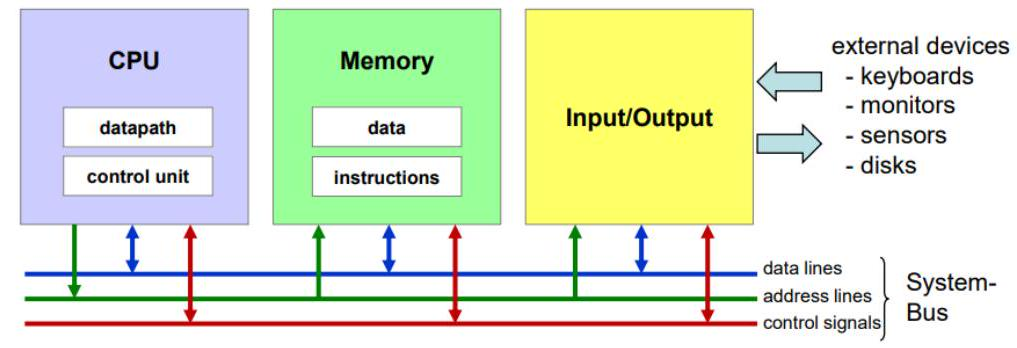
\includegraphics[width=\linewidth]{images/2024_12_29_79e6b22f503fb7b4f718g-01(1)}
\end{definition}

\begin{examplecode}{CPU Components}
The CPU contains several key components:

\textcolor{cornflower}{\textbf{Datapath:}}
\begin{itemize}
  \item \textbf{Core Registers}: Fast but limited storage inside CPU
  \item \textbf{ALU (Arithmetic Logic Unit)}: Performs arithmetic and logic operations
  \end{itemize}
\textcolor{cornflower}{\textbf{Control Unit}}: 
    \begin{itemize}
      \item Finite State Machine: Reads and executes instructions
      \item Controls program flow and manages instruction pipeline
    \end{itemize}
  \textcolor{cornflower}{\textbf{Bus Interface}}: Connects CPU to system bus
\end{examplecode}

\begin{corollary}{Memory} \\
A set of storage cells and the smallest addressable unit is a byte.

$2^N$ addresses:
\begin{itemize}
  \item RAM (Random Access Memory): read/write
  \item ROM (Read-Only Memory): read-only
\end{itemize}
\end{corollary}

\raggedcolumns




\begin{corollary}{Memory Types}
\begin{itemize}
  \item \textbf{Main Memory (Arbeitsspeicher)}:
    \begin{itemize}
      \item Connected through System-Bus
      \item Access to individual bytes
      \item Volatile: 
        \begin{itemize}
          \item SRAM (Static RAM) - faster, more expensive
          \item DRAM (Dynamic RAM) - needs refresh, cheaper
        \end{itemize}
      \item Non-volatile: 
        \begin{itemize}
          \item ROM - factory programmed
          \item Flash - in-system programmable
        \end{itemize}
    \end{itemize}
  \item \textbf{Secondary Storage}:
    \begin{itemize}
      \item Connected through I/O
      \item Access to blocks of data
      \item Non-volatile
      \item Examples: HDD, SSD, CD, DVD
      \item Slower but cheaper than main memory
    \end{itemize}
\end{itemize}
\end{corollary}

\begin{concept}{Memory Addressing}
\begin{itemize}
  \item Each byte in memory has a unique address
  \item Address space depends on address bus width:
    \begin{itemize}
      \item 8-bit address bus: 256 bytes ($2^8$)
      \item 16-bit address bus: 64 KB ($2^{16}$)
      \item 32-bit address bus: 4 GB ($2^{32}$)
    \end{itemize}
  \item Memory map shows allocation of address ranges
\end{itemize}
\end{concept}

\begin{KR}{Key concepts for working with memory}\\
1. Memory terms:
\begin{itemize}
  \item \textbf{Word}: A 32-bit memory unit
  \item \textbf{Half-word}: A 16-bit memory unit
  \item \textbf{Word Alignment}: Address is multiple of word size (4)
\end{itemize}

2. Endianness handling:
\begin{itemize}
  \item \textbf{Little endian}: LSByte at lower address
  \item \textbf{Big endian}: MSByte at lower address
\end{itemize}
\end{KR}

\begin{formula}{Program Translation Process} from C to executable
  \vspace{1mm}\\
Translation from source code to executable involves four steps:

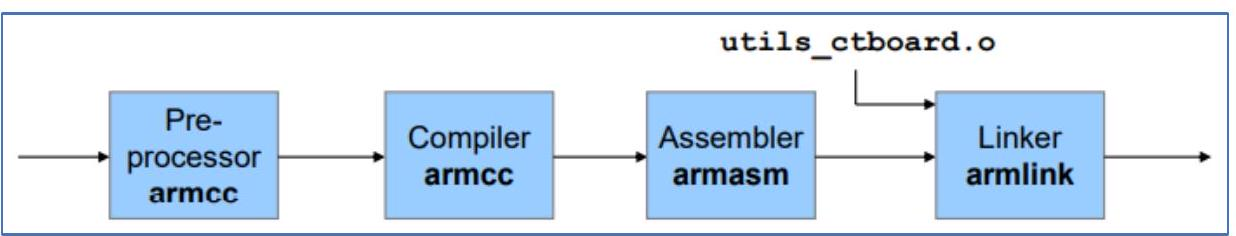
\includegraphics[width=\linewidth]{images/2024_12_29_79e6b22f503fb7b4f718g-01}

\begin{enumerate}
  \item \textbf{Preprocessor}: Text processing
    \begin{itemize}
      \item Includes header files (\#include)
      \item Expands macros (\#define)
      \item Output: Modified source program (.i)
    \end{itemize}
  \item \textbf{Compiler}: Translates C to assembly
    \begin{itemize}
      \item CPU-specific code generation
      \item Optimization (if enabled)
      \item Output: Assembly program (.s)
    \end{itemize}
  \item \textbf{Assembler}: Converts assembly to machine code
    \begin{itemize}
      \item Creates relocatable object file
      \item Generates symbol table
      \item Output: Binary object file (.o)
    \end{itemize}
  \item \textbf{Linker}: Merges object files into executable
    \begin{itemize}
      \item Resolves dependencies
      \item Relocates addresses
      \item Links with libraries
      \item Output: Executable file (.axf)
    \end{itemize}
\end{enumerate}
\end{formula}

\begin{KR}{Program Compilation Process}\\
To compile and link a program:
\begin{enumerate}
  \item Create source files (.c) and header files (.h)
  \item Run preprocessor to expand includes and macros
  \item Compile source files to object files
  \item Link object files and libraries
  \item Test executable
\end{enumerate}

Common compiler flags:
\begin{itemize}
  \item -c: Compile only, don't link
  \item -o: Specify output file name
  \item -O[0-3]: Optimization level
  \item -g: Include debug information
\end{itemize}
\end{KR}

\begin{code}{Simple Program Translation - From Source to Executable}
\begin{lstlisting}[language=C, style=basesmol]
// source.c
#include <stdio.h>
#define MAX 100

int main(void) {
    printf("Max is %d\n", MAX);
    return 0;
}
\end{lstlisting}

After preprocessing (.i):
\begin{lstlisting}[language=C, style=basesmol]
// Contents of stdio.h included here
int main(void) {
    printf("Max is %d\n", 100);
    return 0;
}
\end{lstlisting}

Assembly output (.s):
\begin{lstlisting}[language=armasm, style=basesmol]
    AREA |.text|, CODE, READONLY
    EXPORT main
main
    PUSH {LR}
    LDR R0, =string1
    LDR R1, =100
    BL printf
    MOVS R0, #0
    POP {PC}
    ALIGN
string1 DCB "Max is %d\n",0
    END
\end{lstlisting}
\end{code}

\begin{example2}{Host vs Target Development}\\
When developing for embedded systems:
\begin{itemize}
  \item \textbf{Host}: Development computer where code is written and compiled
  \item \textbf{Target}: Embedded system where code will run
  \item \textbf{Cross-compilation}: Compiling on host for different target architecture
  \item \textbf{Tool chain}: Complete set of development tools (compiler, linker, debugger)
\end{itemize}
\end{example2}

\begin{remark}
Understanding assembly language is important because it:
\begin{itemize}
  \item Helps understand machine-level operation
  \item Aids in debugging and optimization
  \item Required for system programming
  \item Essential for security analysis
\end{itemize}
\end{remark}


	\raggedcolumns
	\subsection{Examples}

\begin{example2}{Was ist Computertechnik?}\\
  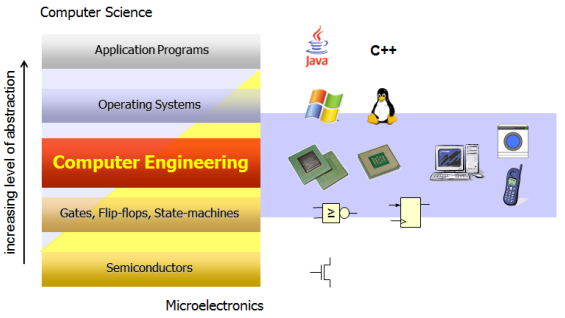
\includegraphics[width=\linewidth]{images/wasistcomputertechniik.png}
\end{example2}

\begin{example2}{Struktur eines Computersystems}\\
Skizzieren Sie die Struktur eines Computersystems:\\
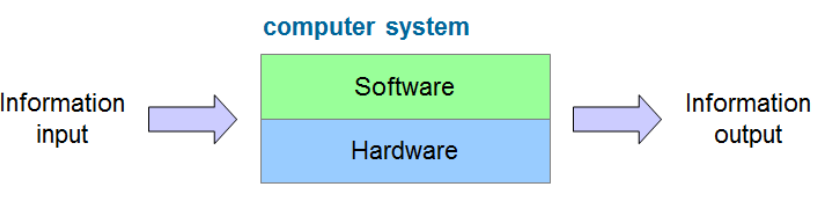
\includegraphics[width=\linewidth]{images/strukturcomputersystem.png}
\end{example2}

\begin{example2}{Komponenten eines Computersystems}\\
Nennen Sie 4 grundlegende Komponenten eines Computersystems und beschreiben Sie die Aufgaben jeder Komponente:
\begin{itemize}
  \item \textbf{CPU (Central Processing Unit)} oder Prozessor: Führt Anweisungen und Daten aus
  \item \textbf{Memory}: Speichert Anweisungen (Instructions) und Daten
  \item \textbf{Input/Output}: Eingabe/Ausgabe Interface zu externen Geräten
  \item \textbf{System Bus}: Elektrische Verbindung von Funktionseinheiten
\end{itemize}
\end{example2}



\begin{example2}{Computer System Components}\\
Examples of basic computer system components and their interactions:

\begin{lstlisting}[language=C, style=basesmol]
// Example showing interaction between components
int main(void) {
    int data;            // Uses Memory
    scanf("%d", &data);  // Uses I/O
    data = data * 2;     // Uses CPU/ALU
    printf("%d", data);  // Uses I/O
    return 0;
}
\end{lstlisting}
\end{example2}

\begin{example2}{Steuereinheit einer CPU}\\
Beschreiben Sie die Aufgaben der Steuereinheit einer CPU:\\
Die Steuereinheit liest, interpretiert und führt Anweisungen aus. Sie steuert den Programmablauf und verwaltet den Befehlsablauf.
\end{example2}

\begin{example2}{von Neumann Architecture}\\
Erklären Sie die von Neumann Architektur:\\
\includegraphics[width=\linewidth]{images/vonneumannerklärung.png}
\end{example2}

\begin{example2}{Programmübersetzung}\\
Nennen und erklären Sie die vier Schritte der Programmübersetzung. Welche Output Dateien werden erzeugt?\\
\textbf{Preprocessor:}
\begin{itemize}
  \item Verarbeitet die Preprocessor Statements (z.B. \#include, \#define)
  \item Textprocessing: Ersetzen und Ergänzen von Inhalten
  \item \textbf{Output:} Textfile mit modifiziertem C Source Code (.i)
\end{itemize}
\textbf{Compiler:}
\begin{itemize}
  \item Übersetzt C Code in prozessorspezifische, symbolische Assemblerbefehle
  \item Optimierung (falls aktiviert)
  \item \textbf{Output:} Textfile mit menschenlesbarem Assemblercode (.s)
\end{itemize}
\textbf{Assembler:}
\begin{itemize}
  \item Übersetzt Assemblercode in binäre Maschinenbefehle
  \item Erzeugt ein Objectfile mit Maschinenbefehlen (relocatable Object File (.o))
\end{itemize}
\textbf{Linker:}
\begin{itemize}
  \item Fügt mehrere Objectfiles zu einem ausführbaren Objectfile zusammen
  \item Löst die entsprechenden Referenzen zwischen den einzelnen Objectfiles auf (Resolution)
  \item Passt Referenzen an die tatsächlichen Speicheradressen an (Relocation)
  \item \textbf{Output:} Ausführbares Objectfile - Executable (.axf)
\end{itemize}
\end{example2}


\begin{example2}{Program Translation Process}\\
Example of program translation stages:

1. Source code (.c):
\begin{lstlisting}[language=C, style=basesmol]
#include <stdio.h>
#define MAX 100

int main(void) {
    printf("Max is %d\n", MAX);
    return 0;
}
\end{lstlisting}

2. After preprocessing (.i):
\begin{lstlisting}[language=C, style=basesmol]
// stdio.h contents included here
int main(void) {
    printf("Max is %d\n", 100);
    return 0;
}
\end{lstlisting}

3. Assembly output (.s):
\begin{lstlisting}[language=armasm, style=basesmol]
    AREA |.text|, CODE, READONLY
    EXPORT main
main
    PUSH    {LR}
    LDR     R0, =string1
    MOV     R1, #100
    BL      printf
    MOVS    R0, #0
    POP     {PC}
string1
    DCB     "Max is %d\n",0
    ALIGN
\end{lstlisting}
\end{example2}

\begin{example2}{Operationstypen CPU}\\
Welche Operationstypen werden im Allgemeinen von einer CPU unterstützt?\\
\includegraphics[width=\linewidth]{images/operationencpuunterstützt.png}
\end{example2}

\begin{example2}{Speicher Typen}\\
Erklären Sie die Unterschiede zwischen Haupt- und Sekundärspeicher.\\
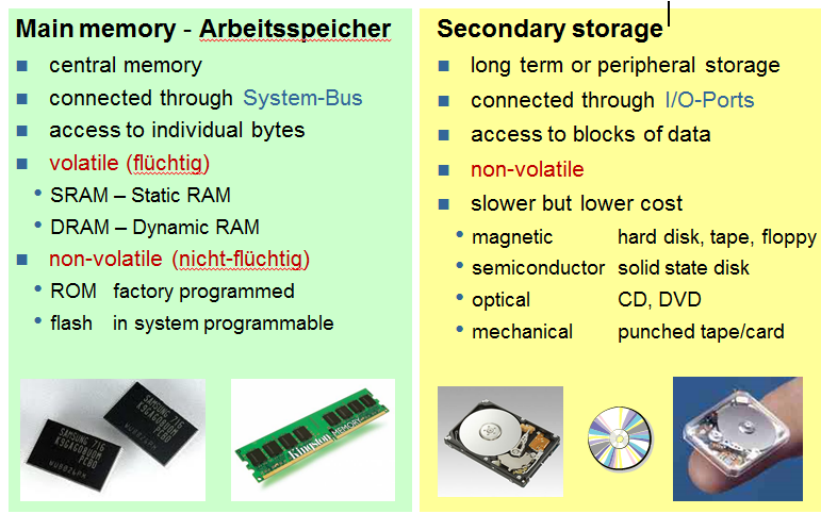
\includegraphics[width=\linewidth]{images/main_secondary_storage.png}
\end{example2}

\begin{example2}{Memory Types and Organization}\\
Example of different memory access patterns:

\begin{lstlisting}[language=armasm, style=basesmol]
; RAM access example
    LDR     R0, =ram_data    ; Load RAM address
    LDR     R1, [R0]         ; Read from RAM
    
; ROM access example
    LDR     R0, =rom_const   ; Load ROM address
    LDR     R1, [R0]         ; Read from ROM
    
; Flash memory programming
    LDR     R0, =FLASH_BASE  ; Flash memory base
    LDR     R1, =0x12345678  ; Data to write
    ; Flash write sequence would go here
    
section_data
ram_data     SPACE   4       ; RAM variable
rom_const    DCD     0xFF    ; ROM constant
\end{lstlisting}
\end{example2}

\begin{KR}{Computer System Debugging}\\
Steps for debugging computer system issues:

1. Hardware level:
\begin{itemize}
  \item Check power and connections
  \item Verify clock signals
  \item Test memory access
  \item Check I/O interfaces
\end{itemize}

2. Software level:
\begin{lstlisting}[language=armasm, style=basesmol]
    ; Debug example
    PUSH    {R0-R3, LR}      ; Save registers
    BL      print_debug      ; Call debug routine
    ; Check specific values
    LDR     R0, =debug_var
    LDR     R1, [R0]
    CMP     R1, #expected
    BNE     error_handler
    POP     {R0-R3, PC}
\end{lstlisting}
\end{KR}

\begin{example2}{PC vs. Embedded System}\\
Erklären Sie den Unterschied zwischen einem Personal Computer (PC) und einem Embedded System bezüglich Aufbau, Anwendung und Programmausführung.\\
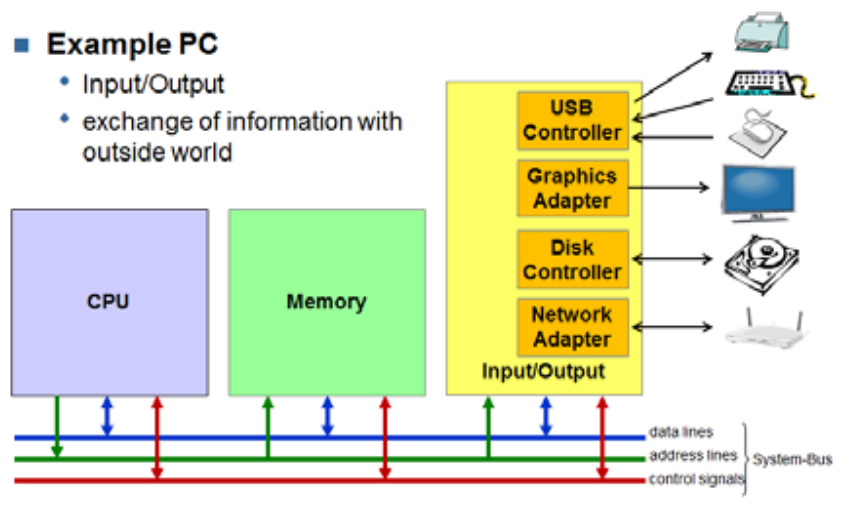
\includegraphics[width=\linewidth]{images/pcexample.png}

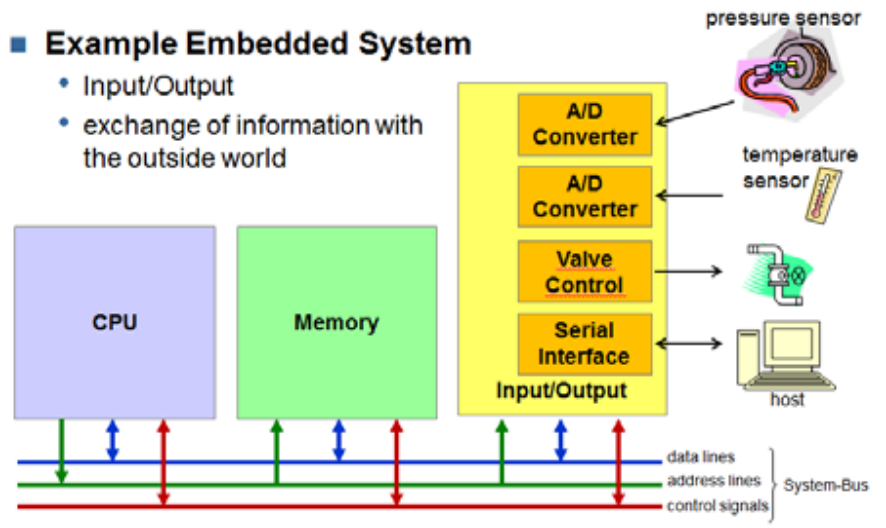
\includegraphics[width=\linewidth]{images/embeddedsystemexample.png}
\end{example2}



\begin{example2}{Wichtigkeit dieses Kurses}\\
Wieso ist Wissen um Assemblerprogrammierung wichtig?
\begin{itemize}
  \item Mit Hilfe von Assembler können wir verstehen, was auf der Maschinenebene abläuft 
  \item Verhalten von Programmen mit Fehlern besser verstehen
  \item Erhöhen der Performance:
  \begin{itemize}
    \item vorhandene und nicht vorhandene Optimierungen durch Compiler verstehen
    \item Ursachen für ineffiziente Programme finden und beheben
  \end{itemize}
  \item Implementieren von System Software: Boot Loader, Betriebssysteme, Interrupt Service Routinen 
  \item Lokalisieren und vermeiden von Sicherheitslücken (z.B. Buffer Overflows)
\end{itemize}
\end{example2}
	\raggedcolumns
	\pagebreak

	\section{Cortex-M Architecture}

\begin{concept}{Core Architecture Overview}\\
The ARM Cortex-M is a 32-bit processor architecture designed for embedded systems:
\begin{itemize}
  \item Load/store architecture
  \item 32-bit data path
  \item Thumb instruction set
  \item Hardware multiply and optional divide
\end{itemize}
\end{concept}

\begin{definition}{Core Registers}\\
The Cortex-M has 16 core registers, each 32-bit wide:
\begin{itemize}
  \item \textbf{R0-R7}: Low registers - general purpose
  \item \textbf{R8-R12}: High registers - general purpose
  \item \textbf{R13 (SP)}: Stack Pointer - temporary storage
  \item \textbf{R14 (LR)}: Link Register - return address from procedures
  \item \textbf{R15 (PC)}: Program Counter - address of next instruction
\end{itemize}
\end{definition}

\begin{definition}{ALU and Flags}\\
The Arithmetic Logic Unit (ALU) is 32-bit wide and supports:
\begin{itemize}
  \item Arithmetic operations (add, subtract, multiply)
  \item Logic operations (AND, OR, XOR)
  \item Compare operations
  \item Shift and rotate operations
\end{itemize}

The Application Program Status Register (APSR) contains flags:
\begin{itemize}
  \item \textbf{N}: Negative result
  \item \textbf{Z}: Zero result
  \item \textbf{C}: Carry from operation
  \item \textbf{V}: Overflow occurred
\end{itemize}
\end{definition}

\begin{definition}{Instruction Set}\\
The Cortex-M uses 16-bit Thumb instructions:

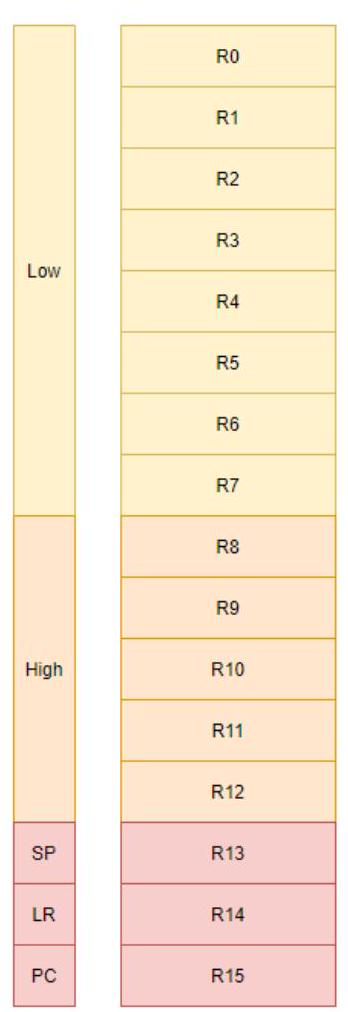
\includegraphics[width=0.35\linewidth, angle=90]{images/2024_12_29_79e6b22f503fb7b4f718g-02}

Main instruction types:
\begin{itemize}
  \item \textbf{Data Transfer}: Move, Load, Store operations
  \item \textbf{Data Processing}: Arithmetic, logical, shift operations
  \item \textbf{Control Flow}: Branch and function calls
\end{itemize}
\end{definition}

\begin{code}{Basic Assembly Program Structure}
Example of a simple assembly program:
\begin{lstlisting}[language=armasm, style=basesmol]
Label   Instr.  Operands   Comments
demoprg MOVS    R0,#0xA5   ;copy 0xA5 into R0
        MOVS    R1,#0x11   ;copy 0x11 into R1
        ADDS    R0,R0,R1   ;add R0 and R1, store in R0
\end{lstlisting}
\end{code}

\begin{concept}{Assembly Program Sections}\\
Program memory is organized in sections:

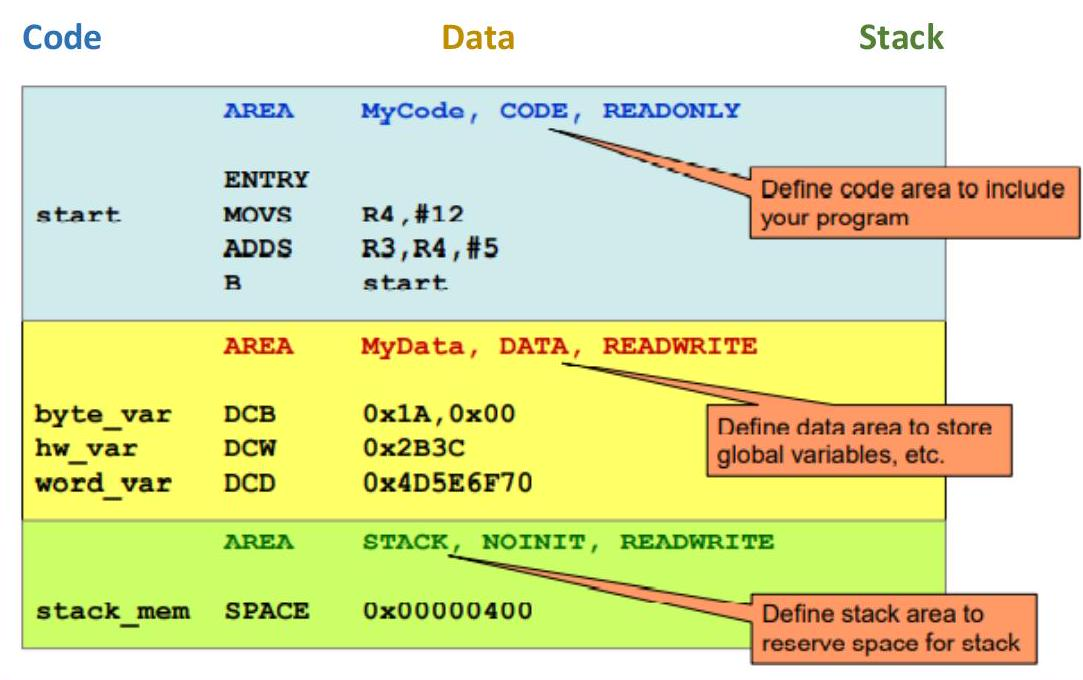
\includegraphics[width=\linewidth]{images/2024_12_29_79e6b22f503fb7b4f718g-02(1)}

\textbf{Directives for initialized data:}
\begin{itemize}
  \item \textbf{DCB}: Define Constant Byte (8-bit)
  \item \textbf{DCW}: Define Constant Half-Word (16-bit)
  \item \textbf{DCD}: Define Constant Word (32-bit)
\end{itemize}

\textbf{Directive for uninitialized data:}
\begin{itemize}
  \item \textbf{SPACE}: Reserve specified number of bytes
\end{itemize}
\end{concept}

\begin{code}{Data Definition}
Memory layout for different data types:
\begin{lstlisting}[language=armasm, style=basesmol]
var1    DCB     0x1A                ;single byte
var2    DCB     0x2B,0x3C,0x4D,0x5E ;byte array
var3    DCW     0x6F70,0x8192       ;half-words
var4    DCD     0xA3B4C5D6          ;word
data    SPACE   100                 ;reserve 100 bytes
\end{lstlisting}
\end{code}

\begin{KR}{Creating Assembly Programs}\\
Steps to create an assembly program:
\begin{enumerate}
  \item Define program sections (CODE, DATA)
  \item Declare any external symbols (IMPORT/EXPORT)
  \item Define initialized data using DCx directives
  \item Reserve uninitialized data using SPACE
  \item Write program code using proper instruction syntax
  \item End program with END directive
\end{enumerate}
\end{KR}
	\raggedcolumns
	\subsection{Examples}

\begin{example2}{CPU Components}\\
Nennen Sie die Hauptkomponenten der M0 CPU und erklären Sie ihre Funktion:
\begin{itemize}
  \item \textbf{Core Registers}:
    \begin{itemize}
      \item 13 x 32-bit Register für temporäre Speicherung (R0 – R12)
      \item 1 x 32-bit Register für Stack Pointer (SP) (R13)
      \item 1 x 32-bit Register für Link Register (LR) (R14)
      \item 1 x 32-bit Register für Program Counter (PC) (R15)
    \end{itemize}
  \item \textbf{ALU} (Arithmetic Logic Unit):
    \begin{itemize}
      \item Data processing unit for arithmetic and logic operations
    \end{itemize}
  \item \textbf{Flags}:
    \begin{itemize}
      \item Processor Status Register: Indicates the state of the processor
    \end{itemize}
  \item \textbf{Control Unit with Instruction Register}:
    \begin{itemize}
      \item Controls execution of an instruction based on the machine code currently stored in the Instruction Register (IR)
    \end{itemize}
  \item \textbf{Bus Interface}:
    \begin{itemize}
      \item Interface between CPU and external System Bus
      \item Bridge between internal and external bus
    \end{itemize}
\end{itemize}
\end{example2}

\begin{example2}{Special Purpose Registers}\\
Beschreiben Sie die Funktion folgender Register:
\begin{itemize}
  \item \textbf{PC (Program Counter)}:
    \begin{itemize}
      \item Points to the address where the instructions will next be read
    \end{itemize}
  \item \textbf{SP (Stack Pointer)}:
    \begin{itemize}
      \item Points to the memory addresses where the elements are written/read from the stack
    \end{itemize}
  \item \textbf{LR (Link Register)}:
    \begin{itemize}
      \item Used to keep track of the positions where to jump back (e.g. routines)
    \end{itemize}
\end{itemize}
\end{example2}

\begin{example2}{Program Counter Initialization}\\
Warum wird der PC bei Reset auf einen definierten Wert initialisiert (während andere CPU Register undefinierte Werte haben können)?\\
So that fetching of the first instruction can always start at the same (known and predictable) place.
\end{example2}

\begin{example2}{M0 Instruction Types}\\
Name 3 instruction types of the M0 CPU:
\begin{itemize}
  \item Data transfer
  \item Data processing
  \item Flow control
\end{itemize}
\end{example2}

\begin{example2}{Instruction Execution Analogy}\\
Ein Prozessor führt eine Liste von Instruktionen in einer vordefinierten Reihenfolge aus. Finden Sie Analogien aus dem Alltag:
\begin{itemize}
  \item Baker/Koch, der einem Rezept folgt
  \item Musiker, der nach Noten spielt
  \item Pilot, der vor dem Start eine Checkliste durchgeht
\end{itemize}
\end{example2}







\begin{example2}{Assembly Code Structure}\\
Name the different parts of a line in assembly code:
\begin{lstlisting}[language=armasm, style=basesmol]
label   MOVS    R0, #42     ; This is a comment
\end{lstlisting}
Components:
\begin{itemize}
  \item Label
  \item Mnemonic (instruction)
  \item Operands
  \item Comment
\end{itemize}
\end{example2}

\begin{example2}{Terms in Memory}
Explain the following terms:
\begin{itemize}
  \item \textbf{Fetch}: Get the instruction from code memory
  \item \textbf{Execute}: Do what the instructions say
  \item \textbf{Word}: A 32-bit memory unit (for the MO)
  \item \textbf{Half-word}: A 16-bit memory unit (for the MO)
  \item \textbf{Little endian}: A multi-byte representation where the LSByte is at the lower address
  \item \textbf{Big endian}: A multi-byte representation where the MSByte is at the lower address
  \item \textbf{Word Alignment}: The address of the multi-byte element is a multiple of the word length (4 for the MO)
  \item \textbf{Data transfer}: Move data between registers and memory
  \item \textbf{Data processing}: Perform arithmetic and logic operations
  \item \textbf{Flow control}: Change the order of execution
  \item \textbf{Stack}: Memory area for procedure calls and local variables
  \item \textbf{Heap}: Memory area for dynamic memory allocation
  \item \textbf{Global variables}: Variables accessible from all functions
  \item \textbf{Local variables}: Variables accessible only within a function
  \item \textbf{Static variables}: Variables with fixed memory allocation
  \item \textbf{Constants}: Fixed values used in the program
  \item \textbf{Code section}: Memory area for instructions
  \item \textbf{Data section}: Memory area for variables
  \item \textbf{Stack section}: Memory area for runtime data
  \item \textbf{Memory map}: Graphical layout showing addresses and sizes of elements
  \item \textbf{Memory areas}: Sections of memory for different purposes
  \item \textbf{Memory sections}: Organized parts of memory for program use
  \item \textbf{Memory ranges}: Address ranges for different memory sections
\end{itemize}
\end{example2}

\columnbreak

\begin{example2}{Memory Map Usage}\\
What is a memory map? What is it used for?
\begin{itemize}
  \item It is a graphical layout (map) showing the addresses and sizes of elements that communicate with the CPU (memories, Inputs, Outputs)
  \item The memory map helps users to know where each element is (e.g. when writing the appropriate drivers)
\end{itemize}
\end{example2}


\begin{example2}{Memory Areas}\\
Which 3 memory areas (sections) can be differentiated for a program?

\begin{itemize}
  \item \textbf{CODE} (read-only → RAM or ROM):
    \begin{itemize}
      \item Machine instructions
      \item Constants
    \end{itemize}
  \item \textbf{DATA} (read-write → RAM):
    \begin{itemize}
      \item Global variables
      \item Static variables
      \item Heap in C
    \end{itemize}
  \item \textbf{STACK} (read-write → RAM):
    \begin{itemize}
      \item Procedure calls
      \item Passing of parameters
      \item Local variables
    \end{itemize}
\end{itemize}
\end{example2}

\begin{example2}{Memory Areas/Memory Map}\\
Assume that the following memory areas are used when executing a program:

\begin{itemize}
  \item Code: $0 \times 20000000$ to $0 x 200001 F F$
  \item Data: 0x20000200 to 0x200002FF
  \item Stack: 0x20000300 to 0x200003FF
\end{itemize}

Draw an appropriate memory map and draw the three sections. Label the first and last addresses for each area. How many storage locations does each of the areas contain?\\

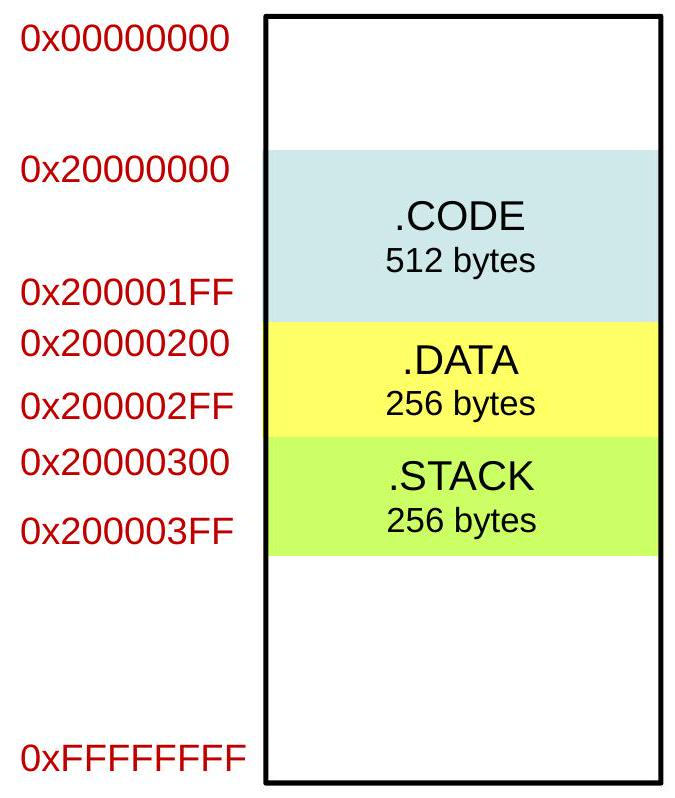
\includegraphics[width=0.6\linewidth]{images/2025_01_02_5d04f07cd96c1366bf1bg-5}
\end{example2}

\begin{KR}{Memory Section Organization}\\
Guidelines for organizing program memory sections:

1. Determine required sections:
\begin{itemize}
  \item Code section for instructions
  \item Data section for variables
  \item Stack section for runtime data
\end{itemize}

2. Calculate section sizes:
\begin{itemize}
  \item Add up all code space needs
  \item Account for all global/static variables
  \item Estimate maximum stack depth
\end{itemize}

3. Assign memory ranges:
\begin{lstlisting}[language=armasm, style=basesmol]
AREA    |.text|, CODE, READONLY
; Code section starts here

AREA    |.data|, DATA, READWRITE
; Data section starts here

; Stack section typically defined in startup code
Stack_Size    EQU     0x400    ; 1KB
AREA    STACK, NOINIT, READWRITE, ALIGN=3
Stack_Mem    SPACE    Stack_Size
\end{lstlisting}
\end{KR}




\begin{example2}{Memory Addressing}\\
Wie viele Memory Bytes können mit verschiedenen Adressbreiten adressiert werden?
\begin{itemize}
  \item 8 bit → 256 Bytes ($2^8$)
  \item 16 bit → 64 KBytes = 65'536 Bytes ($2^{16}$)
  \item 32 bit → 4 GBytes = 4'294'967'296 Bytes ($2^{32}$)
\end{itemize}
\end{example2}



\begin{example2}{Memory addressing}\\
How many byte positions can be addressed by the M0? Which positions in the memory map need to be occupied? Explain your answer.
\vspace{2mm}\\
The M0 has a 32-Bit address bus. Therefore, it can address 4 GByte $=2^{32}$ Bytes. Positions needed for the initialization of the processor (at Boot) must be covered by the proper elements (memory). Otherwise, there will be no correct start.\\
\end{example2}

\begin{example2}{Memory Values Example}\\
A program has variables represented as below in the memory map. Determine the decimal values assuming Little Endian representation:

\begin{tabular}{|l|l|l|}
\hline
Address & Byte content & Variable \\
\hline
0x2FFF´FFF8 & 0xE2 & Var4 (16-bit short) \\
0x2FFF´FFF9 & 01100010 (binary) & \\
\hline
0x2FFF´FFFC & 0x65 & Var3 (32-bit unsigned) \\
0x2FFF´FFFD & 10101101 & \\
0x2FFF´FFFE & 0xA3 & \\
0x2FFF´FFFF & 0x82 & \\
\hline
\end{tabular}

Solutions:
\begin{itemize}
  \item Var4 = 0x62E2 = +25'314d (16-bit signed)
  \item Var3 = 0x82A3AD65 = +2'191'764'837d (32-bit unsigned)
\end{itemize}
\end{example2}



\begin{example2}{Little Endian vs. Big Endian}\\
A program (code in C) has variables represented as below in the memory map. Determine the decimal values of the variables Var1 .... Var5. Assume Little Endian representation.
\begin{center}
\begin{tabular}{|c|c|c|}
\hline
Address & Byte content  & Variable \\
& (decimal, hex, binary) & \\
\hline
0x2FFF'FFF7 & 0x45 &  \\
\hline
0x2FFF'FFF8 & 0xE2 & Var4 (16-bit short) \\
\hline
0x2FFF'FFF9 & 01100010 (binary) &  \\
\hline
0x2FFF'FFFA & 213 &  \\
\hline
0x2FFF'FFFB & 25 &  \\
\hline
0x2FFF'FFFC & 0x65 & Var3 (32-bit  \\
& & unsigned integer) \\
\hline
0x2FFF'FFFD & 10101101(binary) &  \\
\hline
0x2FFF'FFFE & 0xA3 &  \\
\hline
0x2FFF'FFFF & 0x82 &  \\
\hline
0x3000'0000 & 0xA2 & Var5 (32-bit integer) \\
\hline
0x3000'0001 & 34 &  \\
\hline
0x3000'0002 & 0x54 &  \\
\hline
0x3000'0003 & 0xFF &  \\
\hline
0x3000'0004 & 0x92 & Var2 (unsigned char) \\
\hline
$0 \times 3000{ }^{\prime} 0005$ & 0x03 & Var1 (char) \\
\hline
\end{tabular}
\end{center}
Var1 $=0 \times 03=3 d$ (it is 8-bit unsigned)

Var2 $=0 \times 92=146 \mathrm{~d}$ (it is 8 -bit unsigned)

Var3 $=0 \times 82 A 3 A D 65=+2^{\prime} 191^{\prime} 764$ '837d (it is 32-bit unsigned!!)

Var4 $=0 \times 62 \mathrm{E} 2=+25$ '314d (it is 16 -bit signed)

Var5 $=0 x F F 5422 A 2=-1^{\prime} 1263$ '326 (it is 32-bit signed)\\
(-2'147'483'648 + 2'136'220'322)
\vspace{2mm}\\
How would the same variable values be stored on a Big Endian platform? Fill in the table.
\begin{center}
\begin{tabular}{|c|c|c|}
\hline
Address & Byte content & Variable \\
& (decimal, hex, binary) & \\
\hline
0x2FFF'FFF7 & 0x45 &  \\
\hline
0x2FFF'FFF8 & 01100010 (binary) & Var4 (short) \\
\hline
0x2FFF'FFF9 & 0xE2 &  \\
\hline
0x2FFF'FFFA & 213 (or 25) &  \\
\hline
0x2FFF'FFFB & 25 (or 213) &  \\
\hline
0x2FFF'FFFC & 0x82 & Var3 (32-bit  \\
& & unsigned integer) \\
\hline
0x2FFF'FFFD & 0xA3 &  \\
\hline
0x2FFF'FFFE & 10101101(binary) &  \\
\hline
0x2FFF'FFFF & $0 \times 65$ &  \\
\hline
0x3000'0000 & 0xFF & Var5 (32-bit integer) \\
\hline
0x3000'0001 & 0x54 &  \\
\hline
0x3000'0002 & 34 &  \\
\hline
0x3000'0003 & 0xA2 &  \\
\hline
0x3000'0004 & $0 \times 92$ & Var2 (unsigned char) \\
\hline
0x3000'0005 & $0 \times 03$ & Var1 (char) \\
\hline
\end{tabular}
\end{center}
We are not told if 25 / 213 form a unit or not. Therefore, it can be both ways.
\end{example2}




	\raggedcolumns
	\pagebreak
	\section{Data Transfer}

\begin{concept}{Data Transfer Overview}\\
ARM Cortex-M uses a load/store architecture:
\begin{itemize}
  \item Memory can only be accessed through load and store instructions
  \item All other operations work on registers
  \item Various addressing modes for flexible memory access
\end{itemize}
\end{concept}

\begin{formula}{Load Instructions}\\
Main load instructions for moving data into registers:
\begin{itemize}
  \item \textbf{MOVS} (Move and Set flags):
    \begin{itemize}
      \item Register to Register: \texttt{MOVS R1, R2}
      \item 8-bit immediate: \texttt{MOVS R1, \#0x1C}
      \item Constant: \texttt{MOVS R1, \#MyConst}
    \end{itemize}
  \item \textbf{LDR} (Load Register):
    \begin{itemize}
      \item 32-bit literal: \texttt{LDR R1, \#0xA1B2C3D4}
      \item PC-relative: \texttt{LDR R1, [PC, \#12]}
      \item Pseudo instruction: \texttt{LDR R1, =MyConst}
      \item Register indirect: \texttt{LDR R1, [R2]}
    \end{itemize}
  \item \textbf{LDRB} (Load Register Byte):
    \begin{itemize}
      \item Loads 8-bit value
      \item Bits 31 to 8 are set to zero
    \end{itemize}
  \item \textbf{LDRH} (Load Register Half-word):
    \begin{itemize}
      \item Loads 16-bit value
      \item Bits 31 to 16 are set to zero
    \end{itemize}
\end{itemize}
\end{formula}

\begin{formula}{Store Instructions}\\
Instructions for storing data from registers to memory:
\begin{itemize}
  \item \textbf{STR} (Store Register):
    \begin{itemize}
      \item Basic store: \texttt{STR R1, [R2]}
      \item With offset: \texttt{STR R1, [R2, \#0x04]}
    \end{itemize}
  \item \textbf{STRB} (Store Register Byte):
    \begin{itemize}
      \item Stores lowest 8 bits of register
    \end{itemize}
  \item \textbf{STRH} (Store Register Half-word):
    \begin{itemize}
      \item Stores lowest 16 bits of register
    \end{itemize}
\end{itemize}
\end{formula}

\begin{example2}{Memory Access Example}\\
Loading and storing array elements:

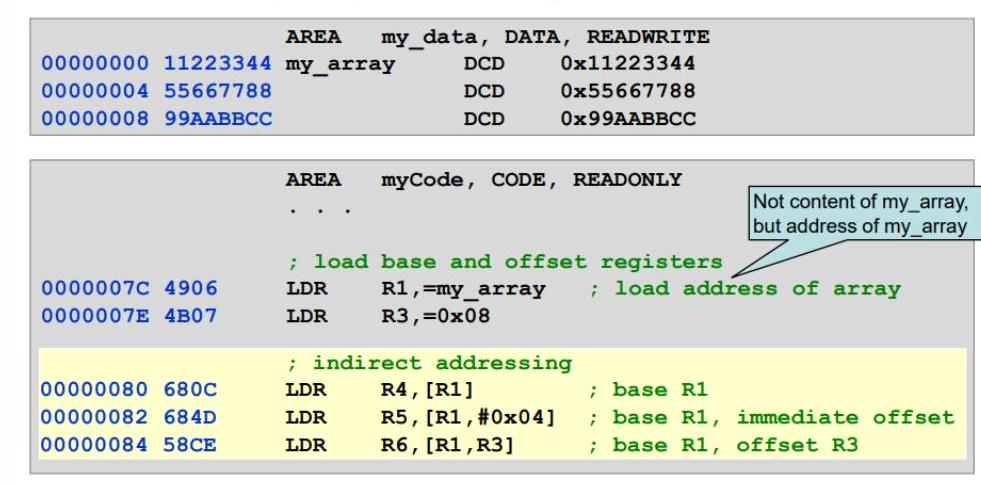
\includegraphics[width=\linewidth]{images/2024_12_29_79e6b22f503fb7b4f718g-03(1)}
\end{example2}

\begin{example2}{Memory Layout Example}\\
Memory layout for array elements and instructions:

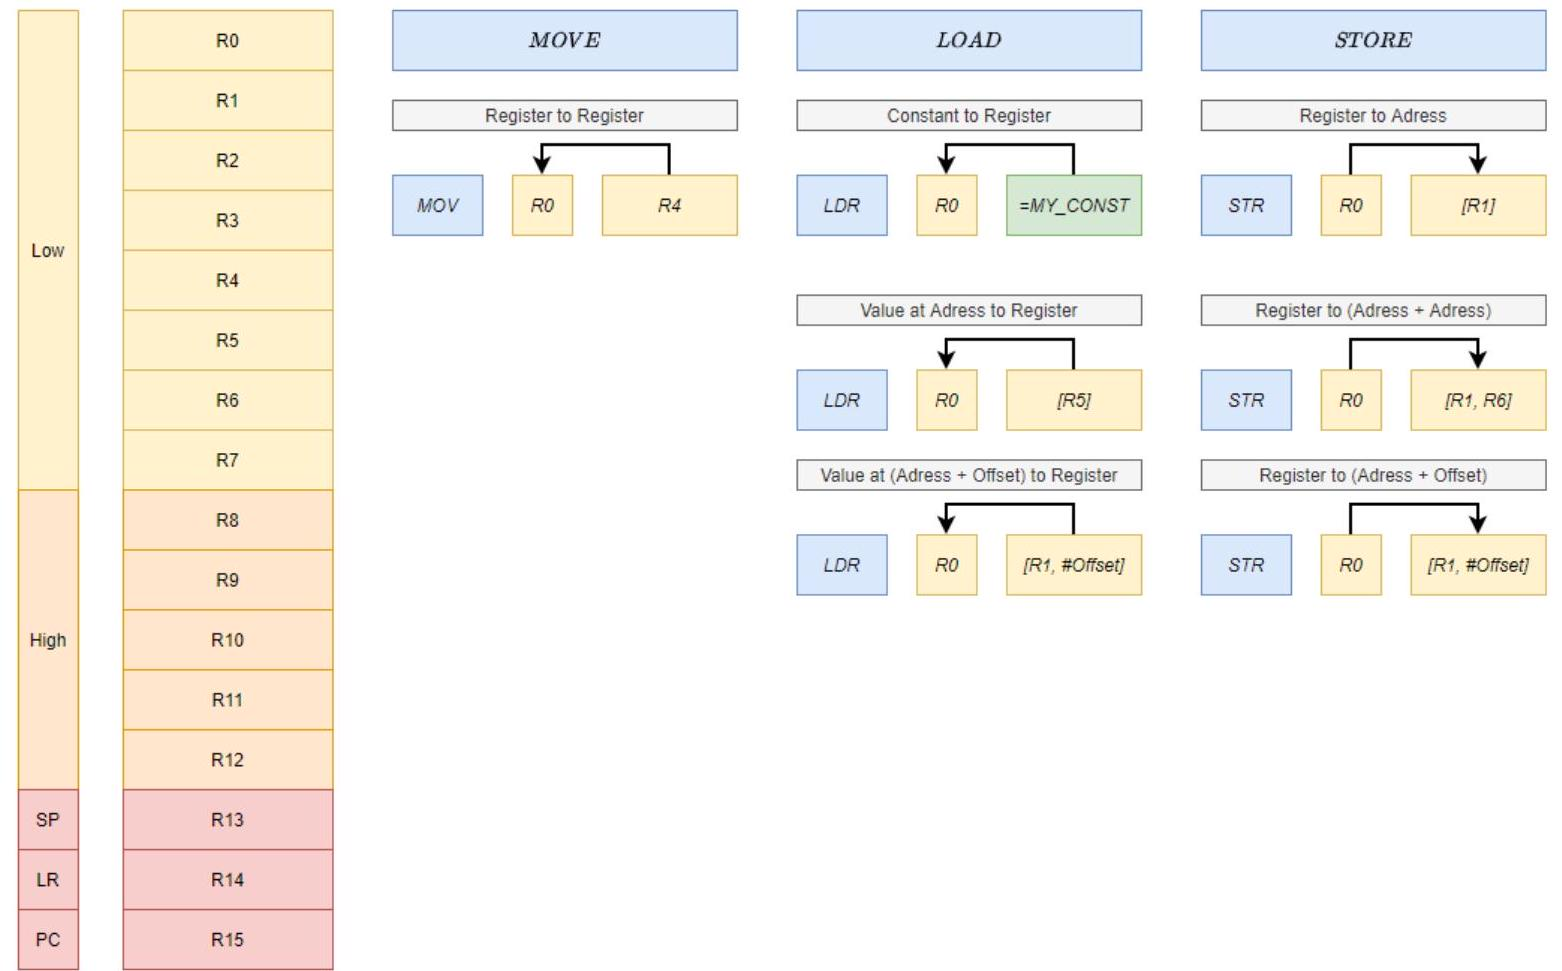
\includegraphics[width=\linewidth]{images/2024_12_29_79e6b22f503fb7b4f718g-03}
\end{example2}
\begin{remark}
Size considerations:
\begin{itemize}
  \item Array elements: 3 * 4 Bytes
  \item Instructions: 5 * 2 Bytes
  \item Literals (0x08): 1 * 4 Bytes
\end{itemize}
\end{remark}

\begin{KR}{Memory Access Patterns}\\
Steps for accessing memory:
\begin{enumerate}
  \item Determine required data size (byte, half-word, word)
  \item Choose appropriate load/store instruction
  \item Calculate correct memory address
  \item Consider alignment requirements
  \item Load/store data using proper addressing mode
\end{enumerate}
\end{KR}

\begin{example2}{Basic Data Transfer Operations}
Common data transfer operations:
\begin{lstlisting}[language=armasm, style=basesmol]
;Load operations
MOVS R1, #42      ;Load immediate value
MOVS R2, R1       ;Copy register
LDR  R3, =0x1234  ;Load 32-bit constant
LDR  R4, [R3]     ;Load from memory
LDRB R5, [R3, #1] ;Load byte with offset

;Store operations
STR  R1, [R2]     ;Store word
STRB R1, [R2, #4] ;Store byte with offset
STRH R1, [R2, R3] ;Store half-word with register offset
\end{lstlisting}
\end{example2}
	\raggedcolumns
	\columnbreak

\subsection{Examples}

\begin{example2}{Load/Store Architecture}
What is a load/store architecture?
\begin{itemize}
  \item Data processing is between registers
  \item Transfer of data from and to the external memory is done using load (memory to register) or store (register to memory) instructions
\end{itemize}
\end{example2}

\begin{example2}{MOV vs MOVS Instructions}\\
Key differences between MOV and MOVS:
\begin{itemize}
  \item \textbf{MOV}: Transfer does NOT affect flags (low and high registers)
  \item \textbf{MOVS}: Transfer affects flags (only low registers)
\end{itemize}
\end{example2}



\begin{example2}{Initializing Registers}\\
Different ways to initialize a register with immediate value:

1. Using MOVS:
\begin{lstlisting}[language=armasm, style=basesmol]
MOVS    R0, #42         ; Limited to 8-bit values
\end{lstlisting}
Advantages:
\begin{itemize}
  \item Value is in instruction
  \item Less memory space needed
\end{itemize}
Disadvantages:
\begin{itemize}
  \item Limited to 8-bit values
  \item Only works with low registers
\end{itemize}

2. Using LDR with PC-relative addressing:
\begin{lstlisting}[language=armasm, style=basesmol]
LDR     R0, [PC, #12]   ; Can load 32-bit values
\end{lstlisting}
Advantages:
\begin{itemize}
  \item Can load larger values (up to 32-bit)
  \item Works with any register
\end{itemize}
Disadvantages:
\begin{itemize}
  \item Takes more space in memory
  \item Requires literal pool management
\end{itemize}
\end{example2}

\begin{example2}{Data transfer instruction for high registers}\\
Which data transfer instructions should you use if at least one high register is an operand?\\
MOV works for all registers (but only for reg/reg transfers)
\end{example2}

\begin{example2}{Initializing low registers}\\
List different ways of initializing a low register with an immediate value. What are the advantages/disadvantages?
\vspace{2mm}\\
\texttt{MOVS <Rd>,\#<imm8>}\\
Value to load is in instruction\\
Less memory space but limited to 8-bit values.
\vspace{2mm}\\
\texttt{LDR <Rt>, [PC,\#<imm>]}\\
Use PC/offset combination to point to the value to load.\\
Can be used to load larger values (up to 32 -bit). Takes more space in memory.
\end{example2}



\begin{KR}{Register Transfer Operations}\\
Steps for data transfer operations:

1. Moving between registers:
\begin{lstlisting}[language=armasm, style=basesmol]
; Copy contents with flags unchanged
MOV     R3, R1          ; For any registers

; Copy contents and update flags
MOVS    R3, R1          ; Only for low registers
\end{lstlisting}

2. Loading immediate values:
\begin{lstlisting}[language=armasm, style=basesmol]
; Small values (flags unchanged)
MOV     R0, #42         ; 8-bit immediate

; Larger values
LDR     R0, =0x12345678 ; 32-bit value using literal pool

; For high registers
LDR     R0, =value      ; Load into low register first
MOV     R8, R0          ; Then move to high register
\end{lstlisting}

3. Memory access:
\begin{lstlisting}[language=armasm, style=basesmol]
; Load from memory
LDR     R0, [R1]        ; Word from address in R1
LDRB    R0, [R1]        ; Byte from address in R1

; Store to memory
STR     R0, [R1]        ; Word to address in R1
STRB    R0, [R1]        ; Byte to address in R1
\end{lstlisting}
\end{KR}

\begin{example2}{Assembly Instructions for Memory Access}\\
Write down the assembly instructions to perform the following actions
\begin{itemize}
  \item Copy contents of R1 in R3 (flags unchanged)\\
  \texttt{MOV R3, R1}
  \item Initialize RO with $0 \times A A$ (flags unchanged)\\
  \texttt{LDR R0,=0xAA}
  \item Initialize R1 with 234 (flags modified)\\
  \texttt{MOVS R1,\#234}
  \item Initialize R4 with $0 \times 55 \mathrm{AACC}$\\
  \texttt{LDR R4,=0x55AACC}
  \item Copy contents of R9 in R3\\
  \texttt{MOV R3, R9}
  \item Initialize R10 with $0 \times 345678$\\
  \texttt{LDR R0,=0x345678 ; R0} as example. \\Another low register is ok:
  \texttt{MOV R10, R0}
  \item Copy contents of R8 in R9\\
  \texttt{MOV R9, R8}
\end{itemize}
\end{example2}



\begin{KR}{Array Access}\\
Guidelines for working with arrays:

1. Calculate element offset:
\begin{itemize}
  \item Byte arrays: offset = index
  \item Half-word arrays: offset = index × 2
  \item Word arrays: offset = index × 4
\end{itemize}

2. Choose appropriate instructions:
\begin{lstlisting}[language=armasm, style=basesmol]
    ; Array base in R0, index in R1
    
    ; For byte array
    LDRB    R2, [R0, R1]    ; index offset
    
    ; For half-word array
    LSLS    R2, R1, #1      ; multiply index by 2
    LDRH    R3, [R0, R2]    ; load half-word
    
    ; For word array
    LSLS    R2, R1, #2      ; multiply index by 4
    LDR     R3, [R0, R2]    ; load word
\end{lstlisting}

3. Consider alignment:
\begin{itemize}
  \item Words must be aligned to 4-byte boundary
  \item Half-words must be aligned to 2-byte boundary
  \item Bytes have no alignment requirement
\end{itemize}
\end{KR}

\begin{remark}
Important considerations:
\begin{itemize}
  \item Always check alignment requirements
  \item Be aware of endianness (STM32 is little-endian)
  \item Consider using multiple register transfer for efficiency
  \item Manage literal pool placement carefully
  \item Stack operations must maintain SP word alignment
\end{itemize}
\end{remark}


\begin{example2}{Pseudo-Instructions}\\
What is a pseudo-Instruction? \\Explain what is done with a <LDR Rn, =literal> pseudo-instruction.
\vspace{2mm}\\
A pseudo-Instruction does not directly translate in machine code. It is an instruction that is interpreted (or expanded)by the assembler (the tool) to generate the needed machine code instruction(s).
\vspace{2mm}\\
When we run the assembler (the tool), the <LDR Rn, =literal> instruction is decomposed into a place reservation of the type DCD and an indirect load of the type LDR <Rt>,[PC,\#<imm>] to get the contents of the reserved position and write it in Rn
\vspace{2mm}\\
Literal can be an address (a position in the memory)\\
Literal can be a constant (the value is known at assembling time)
\end{example2}

\raggedcolumns
\columnbreak

\subsubsection{Memory Access Patterns}

\begin{theorem}{Memory Access Patterns}
Tracking memory and register contents:
\begin{enumerate}
  \item Track register contents:
    \begin{itemize}
      \item Note initial values and update after each instruction
      \item Pay attention to flags if MOVS/ADDS used
    \end{itemize}
  \item Track memory changes: Consider byte ordering! (little-endian)
    \begin{itemize}
      \item Note memory layout before operations
      \item Update after each store instruction
    \end{itemize}
\end{enumerate}
\end{theorem}

\begin{KR}{Analyzing Register Contents and Memory Positions}

1. General Rules for Analysis:
\begin{itemize}
  \item Follow sequential execution order
  \item Track register changes for each instruction
  \item Note immediate values vs. memory loads
  \item Remember ARM is little-endian
  \item Consider word alignment requirements
  \item Account for PC-relative addressing (PC+4)
\end{itemize}

2. Loading Immediate Values:
\begin{lstlisting}[language=armasm, style=basesmol]
    MOVS    R0, #0x42       ; R0 = 0x00000042
    MOVS    R1, #0xFF       ; R1 = 0x000000FF
    
    ; For larger values:
    LDR     R0, =0x12345678 ; Creates literal pool entry
    ; R0 = 0x12345678 (after loading from literal pool)
\end{lstlisting}

3. Direct Memory Access:
\begin{lstlisting}[language=armasm, style=basesmol]
; Given memory at 0x20000000:
; 0x20000000: 78 56 34 12
; 0x20000004: AA BB CC DD

    LDR     R1, =0x20000000 ; R1 = 0x20000000
    LDR     R0, [R1]        ; R0 = 0x12345678 (little-endian!)
    LDR     R2, [R1, #4]    ; R2 = 0xDDCCBBAA
    
    LDRB    R3, [R1]        ; R3 = 0x00000078 (byte access)
    LDRH    R4, [R1]        ; R4 = 0x00005678 (halfword)
\end{lstlisting}

4. PC-Relative Loading:
\begin{lstlisting}[language=armasm, style=basesmol]
    ; At address 0x1000:
    LDR     R0, [PC, #12]   ; PC = 0x1004 for offset
                            ; Loads from 0x1010
    B       next            ; Branch over literal
    DCD     0x12345678      ; At 0x1010
next
    ; R0 = 0x12345678
\end{lstlisting}

5. Register Tracking Table:

\begin{tabular}{|l|l|l|l|}
\hline
Address & Instruction & Register Changes & Memory Changes \\
\hline
0x1000 & MOVS R0,\#1 & R0 = 0x00000001 & None \\
0x1002 & MOVS R1,\#2 & R1 = 0x00000002 & None \\
0x1004 & ADDS R0,R1  & R0 = 0x00000003 & None \\
\hline
\end{tabular}

\end{KR}

\begin{KR}{Analyzing Register Contents and Memory Positions - Continued}

6. Memory Access Patterns:

a) Base + Offset:
\begin{lstlisting}[language=armasm, style=basesmol]
    ; R0 = 0x20000000
    LDR     R1, [R0, #4]    ; Load from 0x20000004
    STR     R2, [R0, #8]    ; Store to 0x20000008
\end{lstlisting}

b) Pre-indexed:
\begin{lstlisting}[language=armasm, style=basesmol]
    ; R0 = 0x20000000
    LDR     R1, [R0, #4]!   ; First updates R0 = 0x20000004
                            ; Then loads from there
\end{lstlisting}

c) Post-indexed:
\begin{lstlisting}[language=armasm, style=basesmol]
    ; R0 = 0x20000000
    LDR     R1, [R0], #4    ; First loads from 0x20000000
                            ; Then updates R0 = 0x20000004
\end{lstlisting}

7. Array Access Analysis:
\begin{lstlisting}[language=armasm, style=basesmol]
    ; Array at 0x20000000: [1,2,3,4]
    ; Memory contents:
    ; 0x20000000: 01 00 00 00 (1 in little-endian)
    ; 0x20000004: 02 00 00 00 (2 in little-endian)
    ; 0x20000008: 03 00 00 00 (3 in little-endian)
    ; 0x2000000C: 04 00 00 00 (4 in little-endian)
    
    LDR     R0, =0x20000000 ; R0 = 0x20000000
    MOVS    R1, #2          ; R1 = 2 (index)
    LSLS    R2, R1, #2      ; R2 = 8 (offset = index * 4)
    LDR     R3, [R0, R2]    ; R3 = 3 (array[2])
\end{lstlisting}

8. Literal Pool Analysis:
\begin{lstlisting}[language=armasm, style=basesmol]
    ; At address 0x1000:
    LDR     R0, =0x12345678 ; Assembler creates:
    B       skip_lit        ; Branch over literal
lit_pool
    DCD     0x12345678      ; Literal pool entry
skip_lit                    ; Continues here
    
    ; Actual machine code:
    ; 0x1000: LDR R0, [PC, #4]  (points to lit_pool)
    ; 0x1002: B skip_lit
    ; 0x1004: 0x12345678        (literal pool)
    ; 0x1008: next instruction   (skip_lit)
\end{lstlisting}

9. Stack Analysis:
\begin{lstlisting}[language=armasm, style=basesmol]
    ; Initial SP = 0x20001000
    PUSH    {R0, R1}        ; SP = 0x20000FF8
                            ; [0x20000FF8] = R0
                            ; [0x20000FFC] = R1
    
    SUB     SP, SP, #8      ; SP = 0x20000FF0
                            ; Allocates 8 bytes
    
    STR     R2, [SP, #0]    ; [0x20000FF0] = R2
    STR     R3, [SP, #4]    ; [0x20000FF4] = R3
\end{lstlisting}
\end{KR}



\begin{example2}{Register Content and Memory Positions} ex 7 from exercise sheet\\
Whenever possible, work out the contents of registers or memory positions that have changed.
\begin{center}
\begin{tabular}{|c|c|c|c|}
\hline
again & LDR & R0, $=0 \times F F$ & \textcolor{darkred}{R0 = 0x000000FF} \\
\hline
 & LDR & R1, lit1 & \textcolor{darkred}{R1 = 0x0000EFAA} \\
\hline
 & LDR & R2, lit2 & \textcolor{darkred}{R2 = 0x00012345} \\
\hline
 & LDR & R3, $=0 \times 55 \mathrm{AA}$ & \textcolor{darkred}{R3 = 0x000055AA} \\
\hline
 & MOV & R4, R1 & \textcolor{darkred}{R4 = 0x0000EFAA} \\
\hline
 & MOV & R4, R2 & \textcolor{darkred}{R4 = 0x00012345} \\
\hline
 & MOV & R6, R3 & \textcolor{darkred}{R6 = 0x000055AA} \\
\hline
 & MOVS & R7, \#04 & \textcolor{darkred}{R7 = 0x00000004} \\
\hline
 & LDR & R0, =lit1 & \begin{tabular}{l}
R0 = address of lit1 \\
(Address is not known) \\
\end{tabular} \\
\hline
 & LDR & R1, =lit2 & \textcolor{darkred}{R1 = address of lit2} \\
\hline
 & LDR & R2, =lit3 & \textcolor{darkred}{R2 = address of lit3} \\
\hline
 & LDRB & R5, [R2] & \textcolor{darkred}{R5 = 0x00000097} \\
\hline
 & LDRH & R6, [R2,\#2] & \textcolor{darkred}{R6 = 0x0000008F} \\
\hline
 & LDR & R2, [R0] & \textcolor{darkred}{R2 = 0x0000EFAA} \\
\hline
 & LDR & R3, [R0, \#4] & \textcolor{darkred}{R3 = 0x00012345} \\
\hline
 & STR & R3, [R1] & \textcolor{darkred}{lit2 = 0x00012345} \\
\hline
 & STR & R2, [R1, \#8] & \textcolor{darkred}{lit4 = 0x0000EFAA} \\
\hline
 & STR & R4, [R1, R7] & \textcolor{darkred}{lit3 = 0x00012345}  \\
 & & & \textcolor{darkred}{(writes to}  \\
 & & & \textcolor{darkred}{(address of lit2 + R7))} \\
\hline
 & LDR & R5, =lit5 & \textcolor{darkred}{R5 = address of lit5} \\
\hline
 & MOVS & R0, \#0 & \textcolor{darkred}{R0 = 0x00000000} \\
\hline
 & ADDS & R7, R0, \#1 & \textcolor{darkred}{R7 = 0x00000001} \\
\hline
 & LDRSB & R6, [R5, R0] & \textcolor{darkred}{R6 = 0xFFFFFF89} \\
\hline
 & LDRSH & R6, [R5, R7] & \textcolor{darkred}{Problem: Unaligned}  \\
 & & & \textcolor{darkred}{memory access} \\
\hline
 & B & Again &  \\
\hline
lit1 & DCD & 0xEFAA &  \\
\hline
lit2 & DCD & 0x12345 &  \\
\hline
lit3 & DCD & 0x8F1097 &  \\
\hline
lit4 & DCD & 0xFF76552F &  \\
\hline
lit5 & DCD & 0xAA654389 &  \\
\hline
lit6 & DCD & 0x0165 &  \\
\hline
Var1 & DCD & 0x23 &  \\
\hline
Var2 & DCD & 0x24 &  \\
\hline
Var3 & DCD & $0 \times 23455678$ &  \\
\hline
Var4 & DCD & 0xE4568900 &  \\
\hline
\end{tabular}
\end{center}
\end{example2}



\begin{formula}
{Common Analysis Mistakes to Avoid}
  \begin{itemize}
    \item \textbf{PC Value}: Remember PC is instruction + 4
    \item \textbf{Endianness}: Memory values are little-endian
    \item \textbf{Alignment}: Check for word/halfword alignment
    \item \textbf{Register Width}: All registers are 32-bit
    \item \textbf{Sign Extension}: Consider for LDR[S]B/LDR[S]H
    \item \textbf{Zero Extension}: Default for regular loads
  \end{itemize}
\end{formula}

\begin{example2}{Memory Access Pattern Example}
Working with arrays and pointers:
\begin{lstlisting}[language=armasm, style=basesmol]
; Array base in R0, index in R1
; Element size 4 bytes (word)
    LSLS    R2, R1, #2      ; R2 = index * 4
    LDR     R3, [R0, R2]    ; Load word from array[index]
    ADDS    R3, #1          ; Increment value
    STR     R3, [R0, R2]    ; Store back to array[index]
\end{lstlisting}
\small
Key points:
\begin{itemize}
  \item Calculate offset = index * element\_size
  \item Use index register for flexible access
  \item Mind alignment requirements
\end{itemize}
\end{example2}



\begin{KR}{PC-Relative Calculations} ex. 8 from exercise sheet\\
Steps for calculating PC-relative offsets:
\begin{enumerate}
  \item Start with instruction address
  \item Add 4 to get effective PC value
  \item Calculate target address
    \begin{itemize}
      \item Must be word-aligned (multiple of 4)
      \item Within ±1KB range
    \end{itemize}
  \item Compute offset = target - (PC + 4)
\end{enumerate}
\begin{lstlisting}[language=armasm, style=basesmol]
; At address 0x1000:
LDR     R0,[PC,#12]       ; PC = 0x1004, loads from 0x1010
...
ALIGN   4
DCD     0x12345678        ; At 0x1010
\end{lstlisting}
\end{KR}

\begin{KR}{Literal Pool Usage} ex. 11 from exercise sheet\\
Steps for working with literals:
\begin{enumerate}
  \item Direct load of value
    \begin{itemize}
      \item LDR Rx,=value for constants
      \item Value stored in literal pool
    \end{itemize}
  \item Load address of label
    \begin{itemize}
      \item LDR Rx,label loads value at label
      \item LDR Rx,=label loads address of label
    \end{itemize}
\end{enumerate}
\begin{lstlisting}[language=armasm, style=basesmol]
    LDR     R0,=0x12345678    ; Load constant from literal pool
    LDR     R1,myvar          ; Load value at myvar
    LDR     R2,=myvar         ; Load address of myvar
    
myvar   DCD     0x11223344     ; Define variable
\end{lstlisting}
\end{KR}

\begin{example2}{String Operations}
Example of byte-wise string copying:
\begin{lstlisting}[language=armasm, style=basesmol]
    ; R0 = source, R1 = destination
copy_loop
    LDRB    R2, [R0]        ; Load byte from source
    ADDS    R0, #1          ; Increment source ptr
    STRB    R2, [R1]        ; Store to destination
    ADDS    R1, #1          ; Increment dest ptr
    CMP     R2, #0          ; Check for null term
    BNE     copy_loop      ; Continue if not done
\end{lstlisting}
\small
Key points: Byte-wise operations, no alignment requirements, null terminator check
\end{example2}

\begin{KR}{Array Traversal Patterns}
Guidelines for iterating through arrays:

1. Forward traversal:
\begin{lstlisting}[language=armasm, style=basesmol]
    ; R0 = array base, R1 = count
    MOVS    R2, #0          ; Initialize index
loop
    LDR     R3, [R0, R2]    ; Load element
    ; Process R3...
    ADDS    R2, #4          ; Next element
    SUBS    R1, #1          ; Decrement counter
    BNE     loop           ; Continue if not done
\end{lstlisting}

2. Post-increment access:
\begin{lstlisting}[language=armasm, style=basesmol]
    ; R0 = array base, R1 = count
loop
    LDR     R3, [R0]        ; Load current
    ADDS    R0, #4          ; Move to next
    ; Process R3...
    SUBS    R1, #1          ; Decrement counter
    BNE     loop           ; Continue if not done
\end{lstlisting}
\end{KR}

\begin{formula}{Array Access} ex. 10 from exercise sheet\\
Steps for array manipulation:
\begin{enumerate}
  \item Calculate array element offset
    \begin{itemize}
      \item Byte arrays: index * 1
      \item Half-word arrays: index * 2
      \item Word arrays: index * 4
    \end{itemize}
  \item Access elements
    \begin{itemize}
      \item LDRB/STRB for bytes
      \item LDRH/STRH for half-words
      \item LDR/STR for words
    \end{itemize}
\end{enumerate}
\end{formula}

\begin{example2}{Array Example}
\begin{lstlisting}[language=armasm, style=basesmol]
LDR     R0,=array         ; Get array base address
MOVS    R1,#1             ; Array index
LSLS    R2,R1,#2         ; Multiply index by 4 (word array)
LDR     R3,[R0,R2]       ; Load array[1]
\end{lstlisting}
\end{example2}

\begin{KR}{Efficient Data Transfer Patterns}
Steps for efficient data movement:

1. Register-to-Register:
\begin{lstlisting}[language=armasm, style=basesmol]
    ; Fast local transfers
    MOV     R1, R0          ; No flags affected
    MOVS    R2, R1          ; Affects flags
\end{lstlisting}

2. Memory-to-Register:
\begin{lstlisting}[language=armasm, style=basesmol]
    ; Choose appropriate size
    LDR     R0, [R1]        ; Word (32-bit)
    LDRH    R0, [R1]        ; Half-word (16-bit)
    LDRB    R0, [R1]        ; Byte (8-bit)
\end{lstlisting}

3. Multiple Register Operations:
\begin{lstlisting}[language=armasm, style=basesmol]
    ; Efficient block transfers
    PUSH    {R0-R3, LR}     ; Save multiple registers
    POP     {R0-R3, PC}     ; Restore and return
\end{lstlisting}
\end{KR}











\begin{KR}{Pointer Arithmetic}
Example demonstrating pointer manipulation:
\begin{lstlisting}[language=armasm, style=basesmol]
    LDR     R0, =array      ; Get array base
    MOVS    R1, #4          ; Element size
    MULS    R2, R4, R1      ; Calculate offset
    
    ; Access array[index]
    ADD     R3, R0, R2      ; Get element address
    LDR     R4, [R3]        ; Load element value
\end{lstlisting}

Key concepts:
\begin{itemize}
  \item Base address in register
  \item Scale index by element size
  \item Maintain proper alignment
\end{itemize}
\end{KR}

\begin{example2}{Handling Pointers}\\
Example C code and assembly implementation:
\begin{lstlisting}[language=C, style=basesmol]
uint32_t x;
uint32_t y;
uint32_t *xp;

void main(void) {
    x = 3;
    xp = &x;
    y = *xp;
}
\end{lstlisting}

Assembly implementation:
\begin{lstlisting}[language=armasm, style=basesmol]
    AREA    myVar, DATA, READWRITE
X   DCD     0
Y   DCD     0
XP  DCD     0

    AREA    myCode, CODE, READONLY
main
    ; Get addresses
    LDR     R3, =X      ; Address of X
    LDR     R4, =Y      ; Address of Y
    LDR     R5, =XP     ; Address of XP
    
    ; x = 3
    MOVS    R0, #3      ; Load immediate value
    STR     R0, [R3]    ; Store in X
    
    ; xp = &x
    STR     R3, [R5]    ; Store address of X in XP
    
    ; y = *xp
    LDR     R2, [R5]    ; Load address from XP
    LDR     R1, [R2]    ; Load value from address
    STR     R1, [R4]    ; Store in Y
\end{lstlisting}
\end{example2}

\begin{comment}
9. In the following C program, code the statements in bold green in assembly.

\begin{verbatim}
// C-Code
uint32_t x;
uint32_t y;
uint32_t *xp;
void main(void) {
    x = 3;
    xp = &x;
    y = *xp;
}
\end{verbatim}

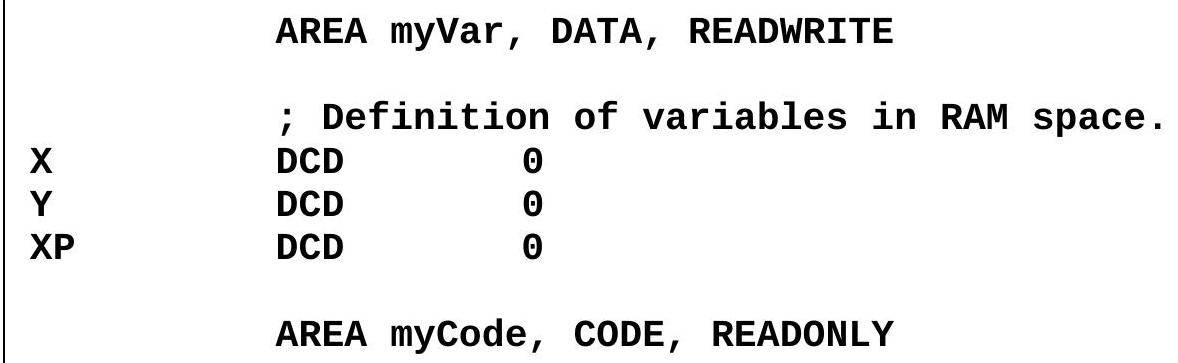
\includegraphics[width=\linewidth]{images/2025_01_02_eeffad754b73de6041b6g-05}\\
main

\begin{verbatim}
; This program is written in order to make it easy to understand
; Efficiency is not the important aspect in this implementation
; First point to variables using registers
LDR R3,=X ; initialize R3 with address of X
    ; reserve place to store address of X in literal pool
LDR R4,=Y ; initialize R4 with address of Y
    ; reserve place to store address of Y in literal pool
LDR R5,=XP ; initialize R5 with address of XP
    ; reserve place to store address of XP in literal pool
; X = 3
LDR R0,=0x03 ; load '3'
STR R0,[R3] ; and store it in X
;XP = &X
STR R3,[R5] ; store address of X (that address is in R3)
    ; in XP (address of XP is in R5)
;Y = *XP
LDR R2,[R5] ; read contents of XP variable (pointed to by
, R5) into R2. Address of X now in R2
LDR R1,[R2] ; read contents of X in R1
STR R1,[R4] ; store R1 (contents of X) in Y (pointed to by R4)
\end{verbatim}

\begin{enumerate}
  \setcounter{enumi}{9}
  \item In the following C program, code the statements in bold green in assembly. Use the frame for solution on following page.
\end{enumerate}

\begin{verbatim}
// C-Code
uint8_t demoArray[2];
uint8_t *xp;
void main(void) {
    demoArray[0] = 10;
    demoArray[1] = 11;
    xp = demoArray;
    *xp = 111;
    xp++;
    *xp = 112;
}
Note: Other statements of the C program are shown in frame with machine code and addresses as examples to help you.
You are only required to write the assembly code (not the machine code).
\end{verbatim}

Frame for solution

Possible solution, as given by the C compiler. This solution does not use pseudo instructions. Before looking at it, make sure that you understand the solution of 9a

22: demoArray[0] = 10;

\begin{center}
\begin{tabular}{|c|c|c|c|}
\hline
0x08000254 & 200A & MOVS & r0,\#0x0A \\
\hline
0x08000256 & 4909 & LDR & r1, [pc,\#36] \\
\hline
0x08000258 & 7008 & STRB & r0, [r1, \#0x00] \\
\hline
23: & \multicolumn{3}{|l|}{demoArray[1] = 11;} \\
\hline
0x0800025A & 200B & MOVS & r0,\#0x0B \\
\hline
0x0800025C & 7048 & STRB & r0, [r1, \#0x01] \\
\hline
\end{tabular}
\end{center}

\begin{center}
\begin{tabular}{|c|c|c|c|}
\hline
\multicolumn{4}{|l|}{24: $\quad \mathrm{xp}=$ demoArray;} \\
\hline
0x0800025E & 4608 & MOV & r0, r1 \\
\hline
0x08000260 & 4907 & LDR & r1, [pc,\#28] \\
\hline
0x08000262 & 6008 & STR & r0, [r1, \#0x00] \\
\hline
$25:$ & \multicolumn{3}{|l|}{${ }^{\text {xp }}$ = 111;} \\
\hline
0x08000264 & 206F & MOVS & r0,\#0x6F \\
\hline
0x08000266 & 6809 & LDR & r1, [r1, \#0x00] \\
\hline
0x08000268 & 7008 & STRB & r0, [r1, \#0x00] \\
\hline
$26:$ & \multicolumn{3}{|l|}{xp++;} \\
\hline
0x0800026A & 4805 & LDR & r0, [pc,\#20] \\
\hline
0x0800026C & 6800 & LDR & r0, [r0, \#0x00] \\
\hline
0x0800026E & 1C40 & ADDS & r0, r0, \#1 \\
\hline
0x08000270 & 4903 & LDR & r1, [pc,\#12] \\
\hline
0x08000272 & 6008 & STR & r0, [r1, \#0x00] \\
\hline
27 : & \multicolumn{3}{|l|}{*xp = 112;} \\
\hline
0x08000274 & 2070 & MOVS & r0,\#0x70 \\
\hline
0x08000276 & 6809 & LDR & r1, [r1, \#0x00] \\
\hline
0x08000278 & 7008 & STRB & r0, [r1, \#0x00] \\
\hline
\end{tabular}
\end{center}

28: \}\\
0x0800027A $4770 \quad$ BX $\quad$ lr ; Not part of solution\\
0x0800027C 0000 DCW 0x0000\\
0x0800027E 2000 DCW 0x2000\\
0x08000280 0004 DCW 0x0004\\
0x08000282 2000 DCW 0x2000\\
This correction shows opcode and assembly instruction to help you understand more. For the solution, only the assembly is required.\\
11. Consider the following listing.

\begin{verbatim}
\begin{tabular}{llll} 
080000008 4804 & again & LDR & R0, lit1 \\
0800000A 480A & & LDR & R0, =lit1 \\
0800000C 4A04 & & LDR & R2, lit2 \\
0800000E 4A0A & & LDR & R2, =lit2 \\
08000010 4B04 & & LDR & R3, lit3 \\
08000012 4C04 & & LDR & R4, lit3 \\
08000014 4E09 & R6, =lit4 \\
08000016 4F09 & & LDR & R7, =lit4 \\
08000018 4408 & & ADD & R0, R1 \\
0800001A E7F5 & B & again
\end{tabular}
0800001C 00000001
xxx DCD 0x01 ; xxx stands for a label
0 8 0 0 0 0 2 0 0 0 0 0 0 0 0 2
    xxx DCD 0x02
0 8 0 0 0 0 2 4 0 0 0 0 0 0 0 3
    xxx DCD 0x03
08000028 00000004
0800002C 00000005
0 8 0 0 0 0 3 0 0 0 0 0 0 0 0 6
08000034
    00000000
    00000000
    00000000
    00000000
\end{verbatim}

a) Compute on the basis of the opcode (marked in blue) the position where data is read to load registers (see table with example)

\begin{center}
\begin{tabular}{|l|l|l|l|}
\hline
\begin{tabular}{l}
Instruction \\
address \\
\end{tabular} & \begin{tabular}{l}
Opcode \\
(marked in blue) \\
\end{tabular} & \begin{tabular}{l}
position where \\
data is read \\
\end{tabular} & \begin{tabular}{l}
Contents of affected \\
register after operation \\
\end{tabular} \\
\hline
08000008 & 4804 & $0 \times 0800001 \mathrm{C}$ & $\mathrm{R0}=0 \times 00000001$ \\
\hline
 &  &  &  \\
\hline
 &  &  &  \\
\hline
 &  &  &  \\
\hline
 &  &  &  \\
\hline
 &  &  &  \\
\hline
 &  &  &  \\
\hline
\end{tabular}
\end{center}

b) The opcodes for <LDR R0, lit1> and <LDR R0, =lit1> are the same. But where are the operands? Explain the differences between the 2 .\\
c) Compute the contents of the registers after each instruction is executed once. Write results in table in a).

Example solutions will be written here

\begin{center}
\begin{tabular}{|l|l|l|l|}
\hline
\begin{tabular}{l}
Instruction \\
address \\
\end{tabular} & Opcode & \begin{tabular}{l}
position where \\
data is read \\
\end{tabular} & \begin{tabular}{l}
Contents of affected \\
register after operation \\
\end{tabular} \\
\hline
08000008 & 4804 & $0 \times 0800001 \mathrm{C}$ & R0 = 0x00000001 \\
\hline
0800000 A & 480A & $0 \times 08000034$ & R0 = 0x0800001C \\
\hline
0800000 C & 4A04 & $0 \times 08000020$ & R2 = 0x00000002 \\
\hline
0800000 E & 4A0A & $0 \times 08000038$ & R2 $=$ 0x08000020 \\
\hline
08000010 & 4B04 & $0 \times 08000024$ & R3 = 0x00000003 \\
\hline
08000012 & 4C04 & $0 \times 08000024$ & R4 = 0x00000003 \\
\hline
08000014 & 4E09 & $0 \times 0800003 C$ & R6 = 0x08000028 \\
\hline
08000016 & 4F09 & 0x0800003C & R7 = 0x08000028 \\
\hline
\end{tabular}
\end{center}

b) <LDR R0, lit1> The value at position label lit1 is loaded in R0\\
<LDR R0, =lit1> Of the form LDR r0, =label\\
(Room is made in the literal pool to store the address of lit1. That address is then loaded in R0 when code is executed)\\
<LDR R0, =const> (e.g. in previous exercise LDR R0, =0xFF55AAB0) Of the form LDR ro, = constant(The constant is placed in a literal pool and loaded in R0)\\
c) see table in a)

Some help to understanding:\\
The code in the processor's memory with comments is shown below\\
$0 \times 080000084804$\\
0x0800000A 480A\\
0x0800000C 4A04\\
0x0800000E 4A0A\\
0x08000010 4B04\\
0x08000012 4C04\\
0x08000014 4E09\\
0x08000016 4F09\\
0x08000018 4408\\
0x0800001A E7F5\\
0x0800001C 0001\\
0x0800001E 0000\\
0x08000020 0002\\
0x08000022 0000\\
0x08000024 0003\\
0x08000026 0000\\
0x08000028 0004\\
0x0800002A 0000\\
0x0800002C 0005\\
0x0800002E 0000\\
0x08000030 0006\\
0x08000032 0000\\
0x08000034 001C\\
0x08000036 0800\\
0x08000038 0020\\
0x0800003A 0800\\
0x0800003C 0028\\
0x0800003E 0800\\
0x08000040 0000\\
0x08000042 0000

\begin{verbatim}
LDR r0,[pc,#16] ; @0x0800001C
    LDR r0,[pc,#40] ; @0x08000034
    LDR r2,[pc,#16] ; @0x08000020
    LDR r2,[pc,#40] ; @0x08000038
        LDR r3,[pc,#16] ; @0x08000024
        LDR r4,[pc,#16] ; @0x08000024
        LDR r6,[pc,#36] ; @0x0800003C
        LDR r7,[pc,#36] ; @0x0800003C
        ADD r0,r0,r1
        B Again (0x08000008)
        DCW 0x0001
        DCW 0x0000
        DCW 0x0002
        DCW 0x0000
        DCW 0x0003
        DCW 0x0000
        DCW 0x0004
        DCW 0x0000
        DCW 0x0005
        DCW 0x0000
        DCW 0x0006
        DCW 0x0000
        DCW 0x001C
        DCW 0x0800
        DCW 0x0020
        DCW 0x0800
        DCW 0x0028
        DCW 0x0800
        DCW 0x0000
        DCW 0x0000
\end{verbatim}

; This is lit1.Value 0x00000001\\
; This is lit2.Value 0x00000002\\
; This is lit3\\
; Address of lit1 stored here\\
; Address of lit2 stored here

Details to the solution for 9a, (given to help you see what is happening).\\
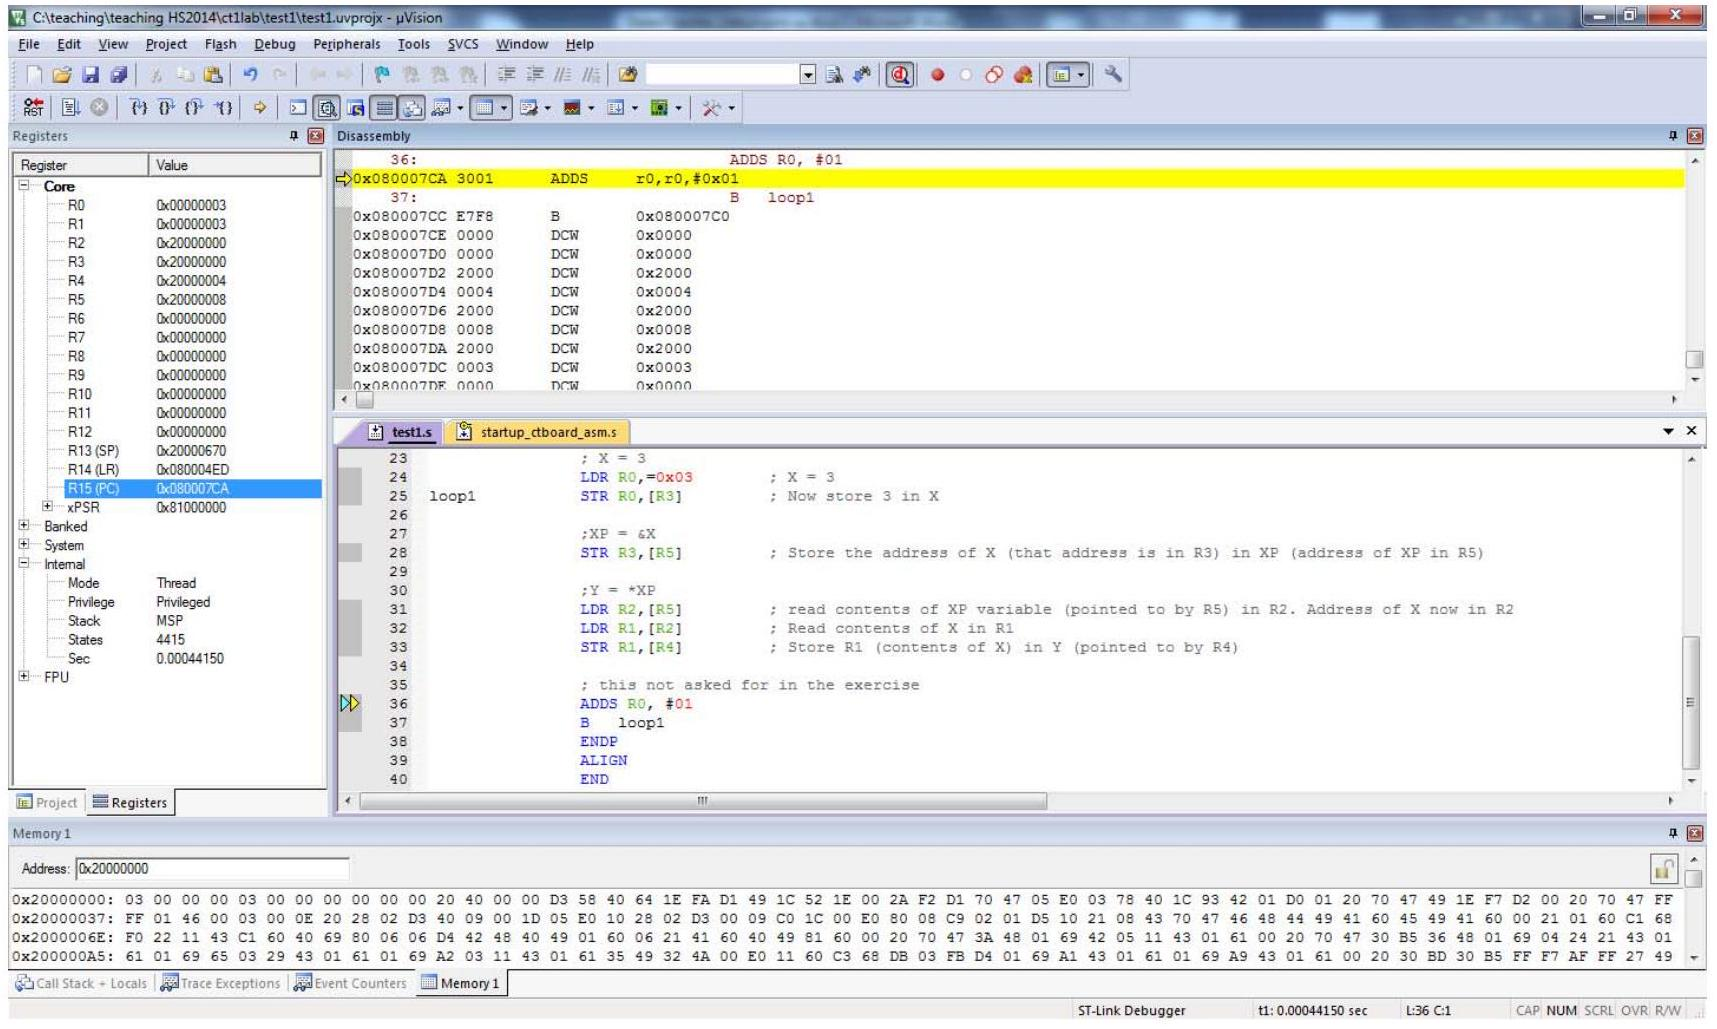
\includegraphics[width=\linewidth]{images/2025_01_02_eeffad754b73de6041b6g-10}

\begin{center}
\begin{tabular}{|c|c|c|c|c|c|}
\hline
19: & \multicolumn{2}{|r|}{LDR R3, = X} & 0x080007B8 4B05 & LDR & r3,[pc,\#20] ; @0x080007D0 \\
\hline
$20:$ & \multicolumn{2}{|r|}{LDR R4,=Y} & 0x080007BA 4C06 & LDR & r4,[pc,\#24] ; @0x080007D4 \\
\hline
21: & \multicolumn{2}{|r|}{LDR R5,=XP} & 0x080007BC 4D06 & LDR & r5,[pc,\#24] ; @0x080007D8 \\
\hline
22: &  &  &  &  &  \\
\hline
23: & \multicolumn{2}{|r|}{; $\mathrm{X}=3$} &  &  &  \\
\hline
24: & \multicolumn{2}{|r|}{LDR R0,=0x03} & 0x080007BE 4807 & LDR & r0,[pc,\#28] ; @0x080007DC \\
\hline
25: loop1 & \multicolumn{2}{|r|}{STR R0,[R3]} & 0x080007C0 6018 & STR & r0,[r3,\#0x00] \\
\hline
26: &  &  &  &  &  \\
\hline
27: & \multicolumn{2}{|r|}{; $\mathrm{XP}=$ \& X} &  &  &  \\
\hline
28: & \multicolumn{2}{|r|}{STR R3,[R5]} & 0x080007C2 602B & STR & r3,[r5,\#0x00] \\
\hline
29: &  &  &  &  &  \\
\hline
30: & \multicolumn{2}{|r|}{; $\mathrm{Y}=$ * XP} &  &  &  \\
\hline
31: & \multicolumn{2}{|r|}{LDR R2,[R5]} & 0x080007C4 682A & LDR & r2,[r5,\#0x00] \\
\hline
32: & \multicolumn{2}{|r|}{LDR R1,[R2]} & 0x080007C6 6811 & LDR & r1,[r2,\#0x00] \\
\hline
33: & \multicolumn{2}{|r|}{STR R1,[R4]} & 0x080007C8 6021 & STR & r1,[r4,\#0x00] \\
\hline
34: &  &  &  &  &  \\
\hline
35: & \multicolumn{3}{|r|}{; this not asked for in the exercise} &  &  \\
\hline
36: & \multicolumn{2}{|r|}{ADDS R0, \#01} & 0x080007CA 3001 & ADDS & r0,r0,\#0x01 \\
\hline
37: & B & loop1 & 0x080007CC E7F8 & B & 0x080007C0 \\
\hline
0x080007CE 0000 & DCW & $0 \times 0000$ &  &  &  \\
\hline
0x080007D0 0000 & DCW & $0 \times 0000$ &  &  &  \\
\hline
0x080007D2 2000 & DCW & $0 \times 2000$ &  &  &  \\
\hline
0x080007D4 0004 & DCW & $0 \times 0004$ &  &  &  \\
\hline
0x080007D6 2000 & DCW & $0 \times 2000$ &  &  &  \\
\hline
0x080007D8 0008 & DCW & $0 \times 0008$ &  &  &  \\
\hline
0x080007DA 2000 & DCW & $0 \times 2000$ &  &  &  \\
\hline
0x080007DC 0003 & DCW & $0 \times 0003$ &  &  &  \\
\hline
0x080007DE 0000 & DCW & $0 \times 0000$ &  &  &  \\
\hline
0x080007E0 0800 & DCW & $0 \times 0800$ &  &  &  \\
\hline
\end{tabular}
\end{center}

Another possible solution for exercise 9 a.\\
As given by the C compiler when code was written in C .\\
Note the MOVS. (This is not always good because it affects flags. So it should be used carefully)

\begin{verbatim}
This solution does not use pseudo instructions
It is here for you to see what the compiler could do
In a normal solution in assembler, it is better to use pseudo
instructions in order to create the literal pool. See solution
above.
The lines in blue are only there for help.
    x = 3;
0x08000254 2003 MOVS r0,#0x03
0x08000256 4905 LDR r1,[pc,#20] ; @0x0800026C
0x08000258 6008 STR r0,[r1,#0x00]
    xp = &x;
0x0800025A 4608 MOV r0,r1
0x0800025C 4904 LDR r1,[pc,#16] ; @0x08000270
0x0800025E 6008 STR r0,[r1,#0x00]
    y = *xp;
0x08000260 4608 MOV r0,r1
0x08000262 6800 LDR r0,[r0,#0x00]
0x08000264 6800 LDR r0,[r0,#0x00]
0x08000266 4903 LDR r1,[pc,#12] ; @0x08000274
\end{verbatim}

\end{comment}

	\raggedcolumns
	\pagebreak
	\section{Arithmetic Operations}

\begin{concept}{Processor Status Flags}\\
APSR (Application Program Status Register) contains important flags affected by arithmetic operations:
\begin{itemize}
  \item \textbf{N} (Negative): Set when result's MSB = 1, used for signed operations
  \item \textbf{Z} (Zero): Set when result = 0, used for both signed/unsigned
  \item \textbf{C} (Carry): Set when unsigned overflow occurs
  \item \textbf{V} (Overflow): Set when signed overflow occurs
\end{itemize}

Instructions ending with 'S' modify these flags:
\begin{itemize}
  \item ADDS, SUBS, MOVS, LSLS
\end{itemize}
\end{concept}

\begin{definition}{Basic Arithmetic Instructions}\\
Core arithmetic operations:
\begin{itemize}
  \item \textbf{ADD/ADDS}: Addition ($A + B$)
  \item \textbf{ADCS}: Addition with Carry ($A + B + c$)
  \item \textbf{ADR}: Address to Register ($PC + A$)
  \item \textbf{SUB/SUBS}: Subtraction ($A - B$)
  \item \textbf{SBCS}: Subtraction with carry/borrow ($A - B - !c$)
  \item \textbf{RSBS}: Reverse Subtract ($-1 \cdot A$)
  \item \textbf{MULS}: Multiplication ($A \cdot B$)
\end{itemize}
\end{definition}

\begin{definition}{Two's Complement}\\
For negative numbers:
\begin{itemize}
  \item Two's complement: $A = !A + 1$
  \item Used for representing signed numbers
  \item Enables using same hardware for addition and subtraction
\end{itemize}
\end{definition}

\begin{concept}{Carry and Overflow}\\
\textbf{Unsigned Operations:}
\begin{itemize}
  \item Addition: C = 1 indicates carry (result too large)
  \item Subtraction: C = 0 indicates borrow (result negative)
\end{itemize}

\textbf{Signed Operations:}
\begin{itemize}
  \item Addition: V = 1 if overflow with operands of same sign
  \item Subtraction: V = 1 if overflow with operands of opposite signs
\end{itemize}
\end{concept}

\begin{example2}{Multi-Word Addition}
Adding 96-bit values using ADCS:

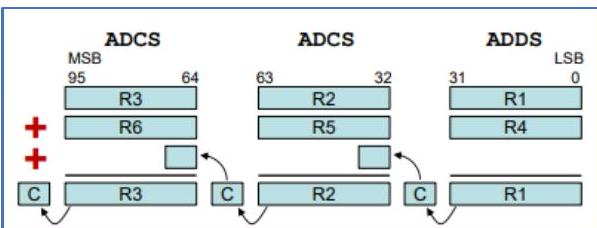
\includegraphics[width=\linewidth]{images/2024_12_29_79e6b22f503fb7b4f718g-04}

\begin{lstlisting}[language=armasm, style=basesmol]
    ADDS R1, R1, R4    ; Add least significant words
    ADCS R2, R2, R5    ; Add middle words with carry
    ADCS R3, R3, R6    ; Add most significant words with carry
\end{lstlisting}
\end{example2}

\begin{example2}{Multi-Word Subtraction}
Subtracting 96-bit values using SBCS:

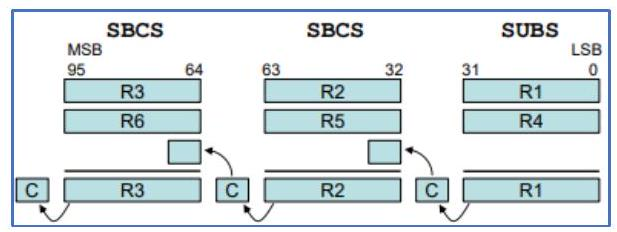
\includegraphics[width=\linewidth]{images/2024_12_29_79e6b22f503fb7b4f718g-04(1)}

\begin{lstlisting}[language=armasm, style=basesmol]
    SUBS R1, R1, R4    ; Subtract least significant words
    SBCS R2, R2, R5    ; Subtract middle words with borrow
    SBCS R3, R3, R6    ; Subtract most significant words with borrow
\end{lstlisting}
\end{example2}

\begin{example2}{Addition and Subtraction Examples}
Addition with carry (13d + 7d):
\begin{verbatim}
  1101  (13d)
  0111  (7d)
  ----
1 0100  (20d = 16d + 4d)
\end{verbatim}

Subtraction with borrow (6d - 14d):
\begin{verbatim}
  0110  (6d)
+ 0010  (TC of 14d)
  ----
  1000  (8d - 16d = -8d)
\end{verbatim}

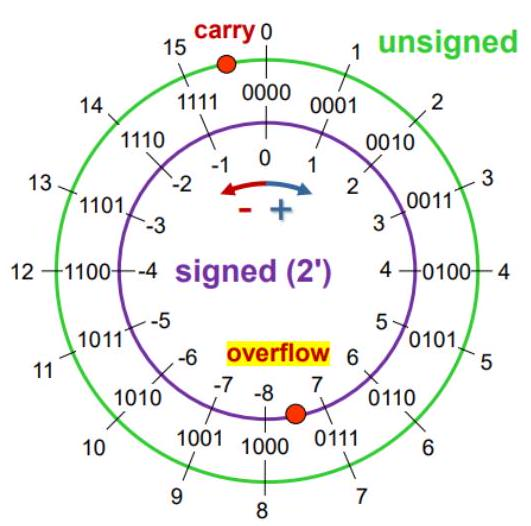
\includegraphics[width=\linewidth]{images/2024_12_29_79e6b22f503fb7b4f718g-04(2)}
\end{example2}

\begin{KR}{Arithmetic Operations}\\
Steps for arithmetic operations:
\begin{enumerate}
  \item Determine if operation is signed or unsigned
  \item Choose appropriate instruction (with or without 'S')
  \item Consider potential carry/overflow conditions
  \item For multi-word operations:
    \begin{itemize}
      \item Start with least significant words
      \item Use carry-aware instructions for higher words
      \item Track flags through operation
    \end{itemize}
  \item Check relevant flags after operation
\end{enumerate}
\end{KR}
	\raggedcolumns
	\pagebreak
	\section{Logic, Shift and Rotate Instructions}

\begin{concept}{Logic Instructions}\\
Base logic operations (affect only N and Z flags):
\begin{itemize}
  \item \textbf{ANDS}: Bitwise AND (Rdn \& Rm, a \& b)
  \item \textbf{BICS}: Bit Clear (Rdn \& !Rm, a \& ~b)
  \item \textbf{EORS}: Exclusive OR (Rdn \textdollar Rm, a $\wedge$  b)
  \item \textbf{MVNS}: Bitwise NOT (!Rm, ~a)
  \item \textbf{ORRS}: Bitwise OR (Rdn \# Rm, a | b)
\end{itemize}
\end{concept}

\begin{example2}{Logical Operations}
Common logic operations:
\begin{lstlisting}[language=armasm, style=basesmol]
; Logic operations
ANDS R0, R1         ; R0 = R0 AND R1
BICS R0, R1         ; R0 = R0 AND NOT R1
EORS R0, R1         ; R0 = R0 XOR R1
MVNS R0, R1         ; R0 = NOT R1
ORRS R0, R1         ; R0 = R0 OR R1

; Shift operations
LSLS R0, R1, #2     ; R0 = R1 << 2 (multiply by 4)
LSRS R0, R1, #1     ; R0 = R1 >> 1 (divide by 2)
ASRS R0, R1, #2     ; R0 = R1 >> 2 (signed divide by 4)
RORS R0, R1, #1     ; Rotate R1 right by 1 bit
\end{lstlisting}
\end{example2}

\begin{concept}{Shift and Rotate Instructions}\\
Shift operations for binary manipulation:
\begin{itemize}
  \item \textbf{LSLS}: Logical Shift Left ($2^n \cdot Rn$, 0 $\rightarrow$ LSB)
  \item \textbf{LSRS}: Logical Shift Right ($2^{-n} \cdot Rn$, 0 $\rightarrow$ MSB)
  \item \textbf{ASRS}: Arithmetic Shift Right ($R^{-n}$, ±MSB $\rightarrow$ MSB)
  \item \textbf{RORS}: Rotate Right (LSB $\rightarrow$ MSB)
\end{itemize}

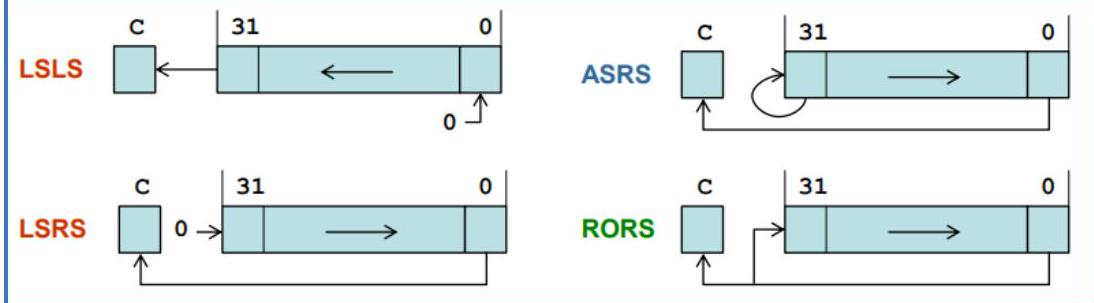
\includegraphics[width=\linewidth]{images/2024_12_29_79e6b22f503fb7b4f718g-06}
\end{concept}

\begin{example2}{Shift Operations for Arithmetic}
Using shifts for multiplication and division:
\begin{lstlisting}[language=armasm, style=basesmol]
; Multiplication by powers of 2
LSLS    R0, R0, #1      ; R0 = R0 * 2
LSLS    R0, R0, #2      ; R0 = R0 * 4
LSLS    R0, R0, #3      ; R0 = R0 * 8

; Division by powers of 2
LSRS    R0, R0, #1      ; R0 = R0 / 2 (unsigned)
ASRS    R0, R0, #1      ; R0 = R0 / 2 (signed)

; Multiply by 10 (8 + 2)
LSLS    R1, R0, #3      ; R1 = R0 * 8
ADDS    R0, R0, R1      ; R0 = R0 + (R0 * 8) = R0 * 9
ADDS    R0, R0, R0      ; R0 = R0 * 2 = R0 * 10
\end{lstlisting}
\end{example2}



\begin{KR}{Using Logic and Shift Instructions}
Steps for bit manipulation:
\begin{enumerate}
  \item Identify required operation (AND, OR, XOR, NOT, shift)
  \item Choose appropriate instruction
  \item Consider effect on flags if relevant
\end{enumerate}

\begin{minipage}[t]{0.55\textwidth}
  \textbf{For shifts:}
    \begin{itemize}
      \item LSLS for multiplication by $2^n$
      \item LSRS for unsigned division by $2^n$
      \item ASRS for signed division by $2^n$
    \end{itemize}
\end{minipage}
\begin{minipage}[t]{0.4\textwidth}
  \textbf{For logic:}
    \begin{itemize}
      \item ANDS for bit masking
      \item ORRS for bit setting
      \item BICS for bit clearing
      \item EORS for bit toggling
    \end{itemize}
\end{minipage}
\end{KR}

\begin{concept}{Flag Behavior with Logic Instructions}\\
Logic instructions only affect N and Z flags:
\begin{itemize}
  \item \textbf{N flag}: Set to bit 31 of result (MSB)
  \item \textbf{Z flag}: Set if result is zero
  \item \textbf{C, V flags}: Unchanged
\end{itemize}

Special case for shift/rotate:
\begin{itemize}
  \item \textbf{C flag}: Set to last bit shifted out
  \item \textbf{N,Z flags}: Set based on result
  \item \textbf{V flag}: Unchanged
\end{itemize}
\end{concept}

\begin{KR}{Bit Manipulation Techniques}\\
Common patterns for bit manipulation:

1. Setting specific bits:
\begin{lstlisting}[language=armasm, style=basesmol]
MOVS    R0, #pattern    ; Create bit pattern
ORRS    target, R0      ; OR to set bits
\end{lstlisting}

2. Clearing specific bits:
\begin{lstlisting}[language=armasm, style=basesmol]
MOVS    R0, #pattern    ; Create bit pattern
BICS    target, R0      ; Clear selected bits
\end{lstlisting}

3. Inverting specific bits:
\begin{lstlisting}[language=armasm, style=basesmol]
MOVS    R0, #pattern    ; Create bit pattern
EORS    target, R0      ; XOR to invert bits
\end{lstlisting}

4. Testing bits:
\begin{lstlisting}[language=armasm, style=basesmol]
MOVS    R0, #pattern    ; Create bit pattern
ANDS    R1, target, R0  ; AND to test bits
; Check flags for result
\end{lstlisting}
\end{KR}

\begin{example2}{Bit Manipulation}
\begin{lstlisting}[language=armasm, style=basesmol]
; Set bits 0 and 4
MOVS    R1, #0x11       ; Mask: 0001 0001
ORRS    R0, R1          ; Set bits in R0

; Clear bits 1 and 5
MOVS    R1, #0x22       ; Mask: 0010 0010
BICS    R0, R1          ; Clear bits in R0

; Toggle bits 2,3,4
MOVS    R1, #0x1C       ; Mask: 0001 1100
EORS    R0, R1          ; Toggle bits in R0

; Test bit 3
MOVS    R1, #0x08       ; Mask: 0000 1000
ANDS    R2, R0, R1      ; Test bit
BEQ     bit_is_clear    ; Branch if bit was 0
\end{lstlisting}
\end{example2}





\subsubsection{Casting, Sign Extension and Type Conversion}

\begin{definition}{Integer Casting}\\
\textbf{Extension (adding bits):}

\begin{minipage}{0.5\textwidth}
\begin{itemize}
  \item \textbf{Zero Extension} (unsigned):
    \begin{itemize}
      \item Fill left bits with zero
      \item Example: 1011 $\rightarrow$ 00001011
    \end{itemize}
\end{itemize}
\end{minipage}
\begin{minipage}{0.5\textwidth}
\begin{itemize}
  \item \textbf{Sign Extension} (signed):
    \begin{itemize}
      \item Copy sign bit to the left
      \item Example: 1011 $\rightarrow$ 11111011
    \end{itemize}
\end{itemize}
\end{minipage}

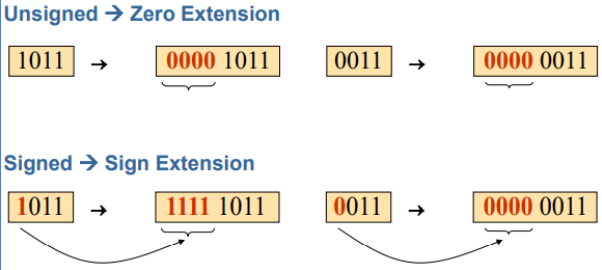
\includegraphics[width=0.7\linewidth]{images/sign_extension.png}

\textbf{Truncation:} Cast cuts out the left most bits
\begin{itemize}
  \item Signed: May change sign
  \item Unsigned: Results in modulo operation
\end{itemize}
\end{definition}

\begin{formula}{Integer Ranges based on word size}\\
  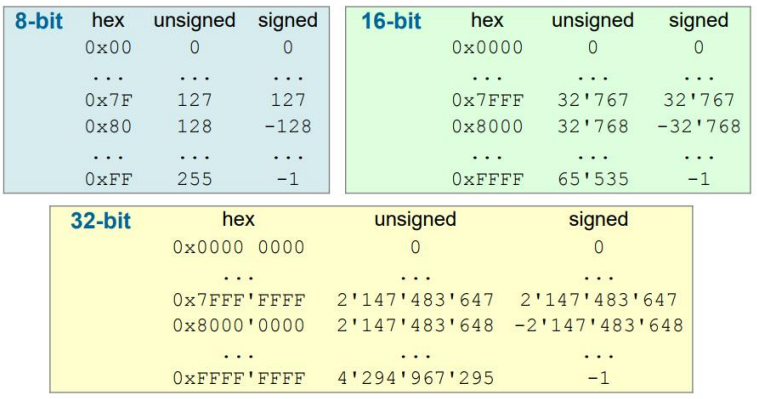
\includegraphics[width=\linewidth]{images/integer_ranges.png}
\end{formula}



\begin{concept}{Sign Extension Instructions}\\
Instructions for extending smaller values:

\begin{minipage}{0.5\textwidth}
\textbf{SXTB}: Sign extend byte to word
    \begin{itemize}
      \item Takes lowest byte
      \item Copies bit 7 to bits 31-8
    \end{itemize}
\textbf{SXTH}: \\Sign extend half-word to word
    \begin{itemize}
      \item Takes lowest half-word
      \item Copies bit 15 to bits 31-16
    \end{itemize}
\end{minipage}
\begin{minipage}{0.5\textwidth}
\textbf{UXTB}: Zero extend byte to word
    \begin{itemize}
      \item Takes lowest byte
      \item Sets bits 31-8 to zero
    \end{itemize}
\textbf{UXTH}:\\ Zero extend half-word to word
    \begin{itemize}
      \item Takes lowest half-word
      \item Sets bits 31-16 to zero
    \end{itemize}
\end{minipage}
\end{concept}

\begin{example2}{Sign Examples}
\begin{lstlisting}[language=armasm, style=basesmol]
; Sign extension examples
SXTB    R0, R1          ; Sign extend byte
SXTH    R0, R1          ; Sign extend half-word

; Zero extension examples
UXTB    R0, R1          ; Zero extend byte
UXTH    R0, R1          ; Zero extend half-word

; Manual sign extension
LSLS    R0, R0, #24     ; Shift left 24 bits
ASRS    R0, R0, #24     ; Arithmetic shift right 24
\end{lstlisting}
\end{example2}

\begin{KR}{Type Conversion Guidelines}
Steps for safe type conversion:

1. For unsigned to larger unsigned:
\begin{itemize}
  \item Use zero extension (UXTB, UXTH)
  \item Or use LSLS followed by LSRS
\end{itemize}

\begin{lstlisting}[language=armasm, style=basesmol]
  ; Extend 8-bit to 32-bit unsigned
  MOVS    R0, #0xFF       ; Load 8-bit value
  UXTB    R2, R0          ; Unsigned extension
  
  ; Manual zero extension
  LDRB    R0, [R1]       ; Load byte, top bits zero
  LSLS    R0, #24        ; Move to top byte
  LSRS    R0, #24        ; Logical shift back
\end{lstlisting}

2. For signed to larger signed:
\begin{itemize}
  \item Use sign extension (SXTB, SXTH)
  \item Or use LSLS followed by ASRS
\end{itemize}

\begin{lstlisting}[language=armasm, style=basesmol]
  ; Extend 8-bit to 32-bit signed
  MOVS    R0, #0xFF       ; Load 8-bit value
  SXTB    R1, R0          ; Signed extension
  
  ; Manual sign extension
  LDRSB   R0, [R1]       ; Load with sign extend
  LDRB    R0, [R1]       ; Load byte
  LSLS    R0, #24        ; Move to top byte
  ASRS    R0, #24        ; Arithmetic shift back
\end{lstlisting}


3. Reducing size (truncation):
\begin{itemize}
  \item Use AND with appropriate mask
  \item Or store using STRB/STRH
  \item Check for potential data loss
\end{itemize}


Example:
\begin{lstlisting}[language=armasm, style=basesmol]
    ; Truncate 32-bit to 8-bit
    MOVS    R1, #0xFF       ; Create mask
    ANDS    R0, R1          ; Truncate to 8 bits

    ; Store 32-bit value as 8-bit
    STRB    R0, [R1]        ; Store byte 
\end{lstlisting}
%TODO: check if this is correct
\end{KR}


\raggedcolumns

\begin{remark}
Important considerations:
\begin{itemize}
  \item Always consider signedness of values
  \item Check for potential carry/overflow in arithmetic shifts
  \item Remember carry flag behavior in shifts
  \item Use appropriate extension for data type
  \item Consider performance impact of shifts vs multiply
  \item Be careful with bit patterns crossing byte boundaries
  \item Document complex bit manipulations clearly
\end{itemize}
\end{remark}




	\raggedcolumns
	\subsection{Examples}



\begin{example2}{Logical Instructions}\\
Bit manipulation examples:

1. Inverting register contents (one's complement):
\begin{lstlisting}[language=armasm, style=basesmol]
MVNS    R1, R1          ; Invert all bits in R1
\end{lstlisting}

2. Selective bit manipulation:
\begin{lstlisting}[language=armasm, style=basesmol]
; Set bits 3..0 to 1, bits 7..4 to 0
; Invert bits 17-16, keep others unchanged
MOVS    R0, #0xF     ; Pattern for bits 3..0
ORRS    R1, R0       ; Set bits 3..0 to 1
MOVS    R0, #0xF0    ; Pattern for bits 7..4
BICS    R1, R0       ; Clear bits 7..4
MOVS    R0, #0x30       
LSLS    R0, #12      ; 0x30000 shift 4 nibbles = 12bit
EORS    R1, R0       ; Invert bits 17-16
\end{lstlisting}
\end{example2}

\raggedcolumns



\begin{example2}{Multiplication Using Shifts}\\
Multiply R7 by 43 using two different methods:

1. Using multiplication instruction:
\begin{lstlisting}[language=armasm, style=basesmol]
MOVS    R0, #43         ; Load constant
MULS    R7, R0, R7      ; Multiply
\end{lstlisting}

2. Using shifts and additions:
\begin{lstlisting}[language=armasm, style=basesmol]
MOVS    R7, R0          ; Copy original value
LSLS    R0, R0, #1      ; *2
ADDS    R7, R7, R0
LSLS    R0, R0, #2      ; *8=4*2
ADDS    R7, R7, R0
LSLS    R0, R0, #2      ; *32=8*4
ADDS    R7, R7, R0      ; Total = 1 + 2 + 8 + 32 = 43
\end{lstlisting}
\end{example2}

\begin{example2}{Reverse Engineering}\\
Convert assembly to C code:

Given C variables:
\begin{lstlisting}[language=C, style=basesmol]
uint32_t ux, uy, uz;    // Variables in memory
\end{lstlisting}

Example 1:
\begin{lstlisting}[language=armasm, style=basesmol]
; Assembly code
LDR     R0, =ux         ; Load address
LDR     R1, [R0]        ; Load value
LSLS    R1, R1, #1      ; Shift left by 1
LDR     R2, =uy         ; Load uy address
LDR     R3, [R2]        ; Load uy value
ADDS    R3, R1          ; Add shifted ux
LSLS    R3, R3, #3      ; Shift left by 3
STR     R3, [R2]        ; Store back in uy
\end{lstlisting}

Equivalent C code:
\begin{lstlisting}[language=C, style=basesmol]
uy = ((ux << 1) + uy) << 3;
// or: 
uy = 8 * (2 * ux + uy);
\end{lstlisting}
\end{example2}

\begin{example2}{Reverse Engineering 2}\\
Convert assembly to C code:

Die Speicherstellen im Assembler werden den ursprünglichen Variablen im C-Programm wie folgt zugeordnet:
\begin{lstlisting}[language=armasm, style=basesmol]
ux: DCD ? ; uint32_t ux
uy: DCD ? ; uint32_t uy
uz: DCD ? ; uint32_t uz
\end{lstlisting}

Example 2:
\begin{lstlisting}[language=armasm, style=basesmol]
; Assembly code
LDR     R0, =ux         ; Load address
LDR     R1, [R0]        ; Load value
LDR     R2, =uy         ; Load address
LDR     R3, [R2]        ; Load value
LDR     R4, =uz         ; Load address
LDR     R5, [R4]        ; Load value
LSRS    R1, R1, #3      ; Shift right by 3
LSLS    R3, R3, #4      ; Shift left by 4
ORRS    R1, R3          ; OR to combine
MVNS    R1, R1          ; Invert bits
ANDS    R1, R5          ; AND with uz
STR     R1, [R4]        ; Store back in uz
\end{lstlisting}

Equivalent C code:
\begin{lstlisting}[language=C, style=basesmol]
uz = ~( (ux >> 3) | (uy << 4)) & uz;
// or:
uz = ~( (ux / 8) | (uy * 16)) & uz;
\end{lstlisting}
\end{example2}

\begin{example2}{Type Casting}
Examples of explicit casting in C:
\vspace{1mm}\\
1. Unsigned to signed casting:
\begin{lstlisting}[language=C, style=basesmol]
uint8_t ux = 100;           // 0x64 or 0110 0100
int8_t sx = (int8_t)ux;     // Same bit pattern
                            // Interpreted as 100
\end{lstlisting}

Als welche Dezimalzahl wird der Inhalt der Variable sx nach dem Cast interpretiert?
\vspace{1mm}\\
100d --> ux hat Speicherinhalt 0x64 oder Binär 0110'0100
\vspace{1mm}\\
sx hat denselben Speicherinhalt, wird aber als signed
interpretiert. Da das höchstwertigste Bit nicht gesetzt ist, hat die
Interpretation aber in diesem Fall keinen Einfluss.
\vspace{1mm}\\
sx wird ebenfalls als 100d interpretiert
\vspace{2mm}\\
2. Signed to unsigned casting:
\begin{lstlisting}[language=C, style=basesmol]
int8_t sx = -10;           // 0xF6 or 1111 0110
uint8_t ux = (uint8_t)sx;  // Same bits but unsigned
                           // 246 (128+64+32+16+4+2)
\end{lstlisting}

Als welche Dezimalzahl wird der Inhalt der Variable ux nach dem Cast interpretiert?
\vspace{1mm}\\
-10d --> sx hat Speicherinhalt 0xF6 oder Binär 1111'0110
(-128+64+32+16+4 + 2)
\vspace{1mm}\\
ux hat denselben Speicherinhalt, wird aber als unsigned
interpretiert. So ergibt sich 128 + 64 + 32 + 16 + 4 + 2 = 246d
\end{example2}








	\raggedcolumns
	\pagebreak
	\section{Control Structures}

\begin{concept}{Branch Instructions}\\
Branch instructions control program flow:

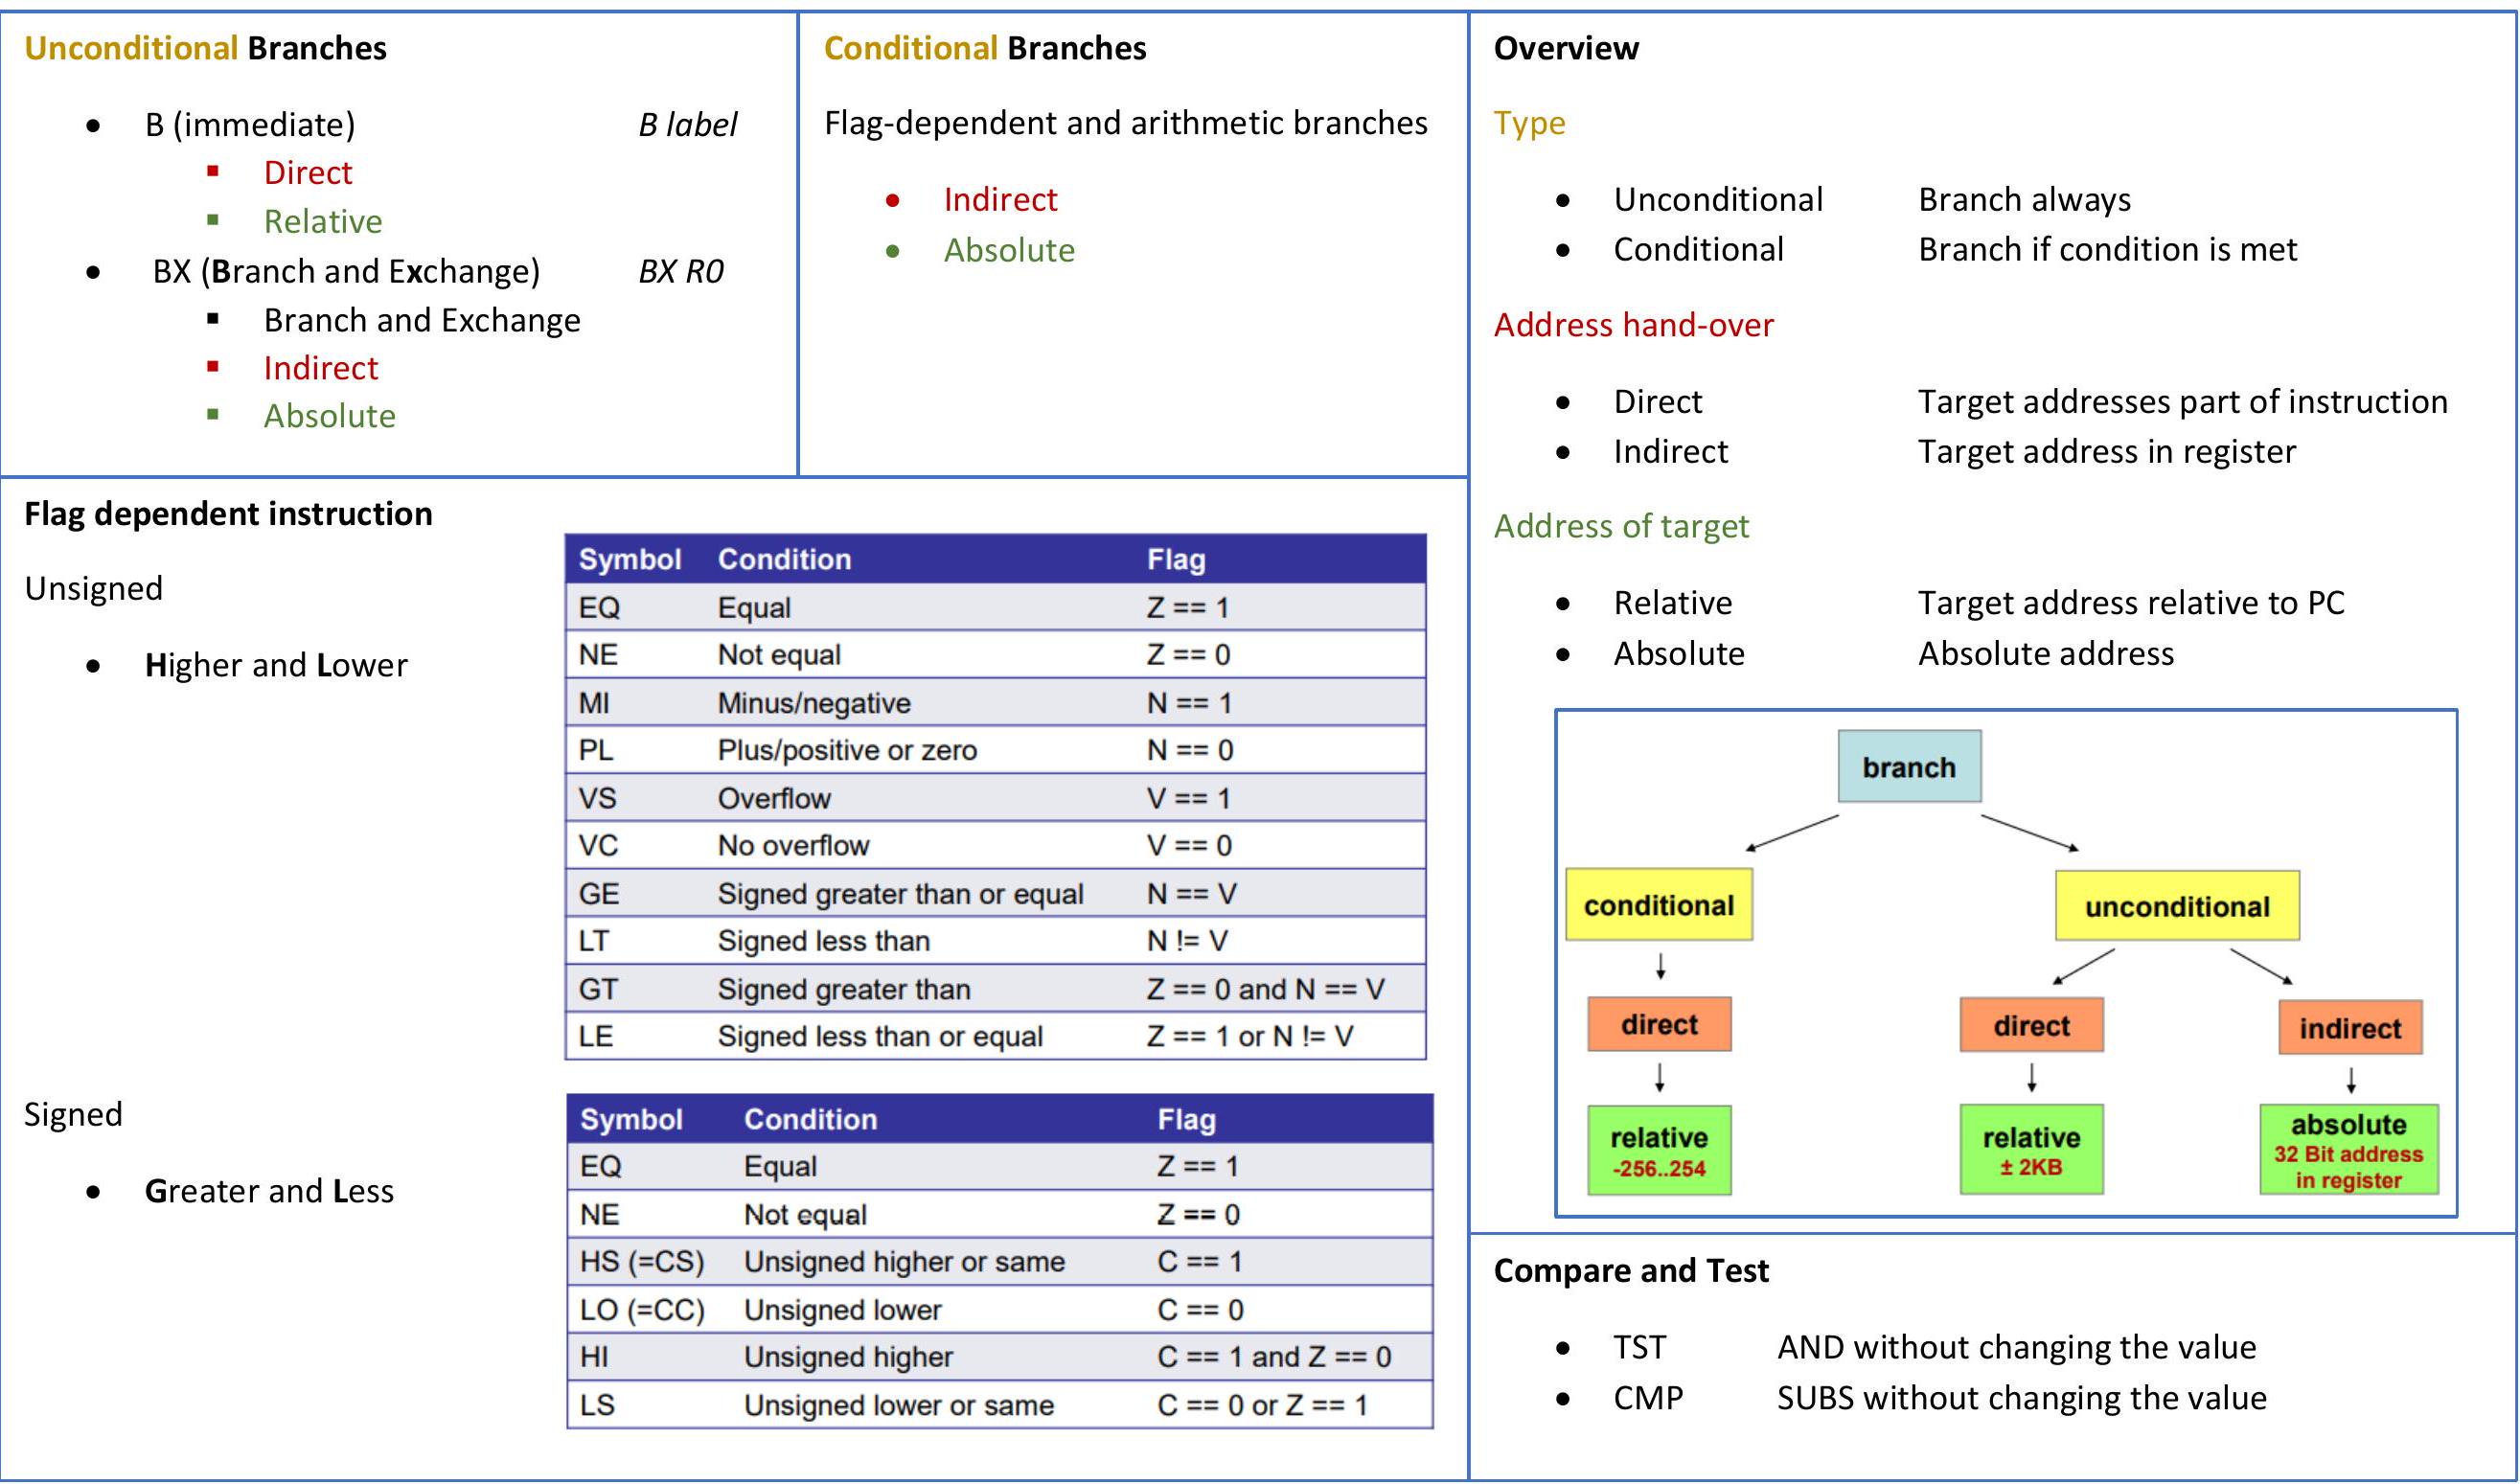
\includegraphics[width=\linewidth]{images/2024_12_29_79e6b22f503fb7b4f718g-05}

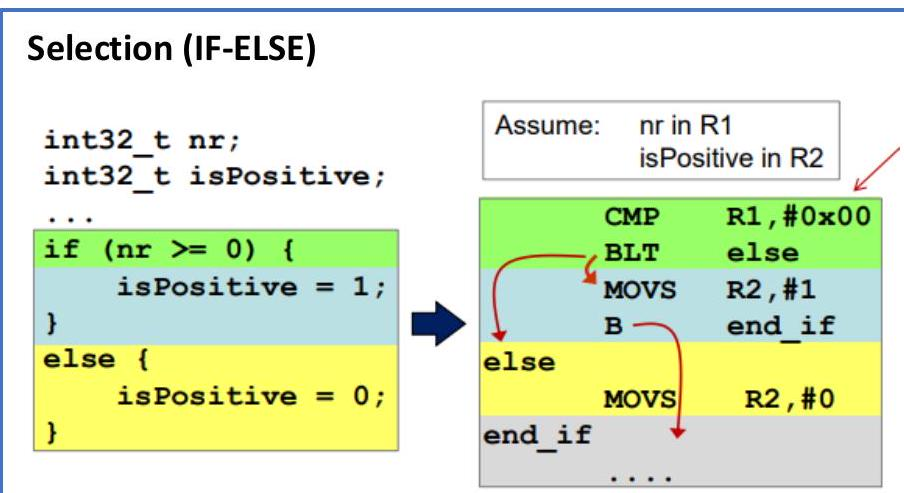
\includegraphics[width=\linewidth]{images/2024_12_29_79e6b22f503fb7b4f718g-07(3)}
\end{concept}

\begin{example2}{Switch Statement Implementation}
C code example:
\begin{lstlisting}[language=C, style=basesmol]
uint32_t result, n;
switch (n) {
    case 0:
        result += 17;
        break;
    case 1:
        result += 13;
        //fall through
    case 3: 
    case 5:
        result += 37;
        break;
    default:
        result = 0;
}
\end{lstlisting}

Assembly implementation with jump table:
\begin{lstlisting}[language=armasm, style=basesmol]
NR_CASES    EQU     6
case_switch CMP     R1, #NR_CASES
            BHS     case_default
            LSLS    R1, #2        ; * 4
            LDR     R7, =jump_table
            LDR     R7, [R7, R1]
            BX      R7

case_0      ADDS    R2, R2, #17
            B       end_sw_case
case_1      ADDS    R2, R2, #13
case_3_5    ADDS    R2, R2, #37
            B       end_sw_case
case_default MOVS   R2, #0
end_sw_case ...

jump_table  DCD     case_0
            DCD     case_1
            DCD     case_default
            DCD     case_3_5
            DCD     case_default
            DCD     case_3_5
\end{lstlisting}
\end{example2}

\begin{concept}{Loop Types}\\
Three main types of loops:

\textbf{Do-While (Post-Test Loop)}:
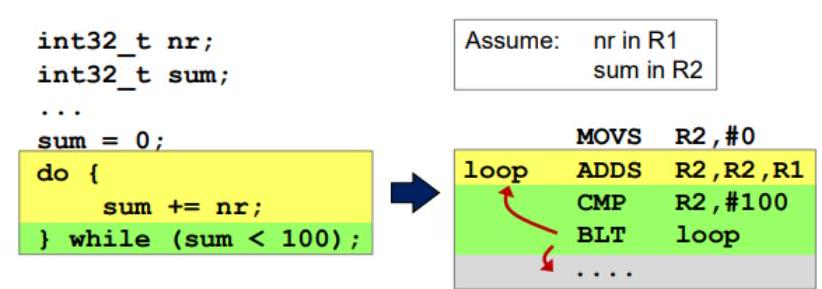
\includegraphics[width=\linewidth]{images/2024_12_29_79e6b22f503fb7b4f718g-07}

\textbf{While (Pre-Test Loop)}:
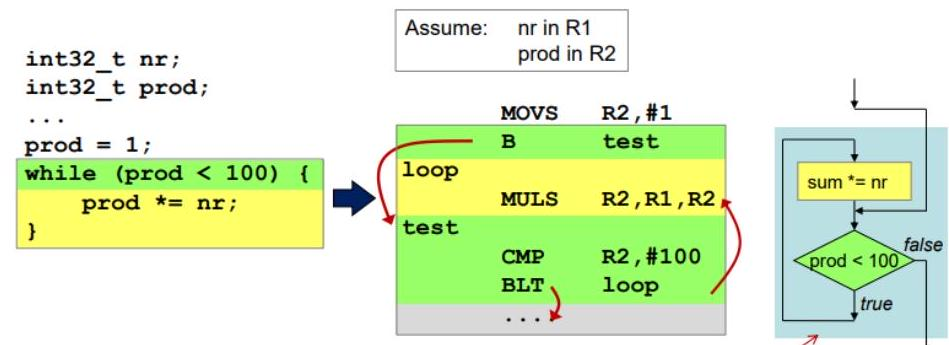
\includegraphics[width=\linewidth]{images/2024_12_29_79e6b22f503fb7b4f718g-07(1)}

\textbf{For Loop (Pre-Test Loop)}:
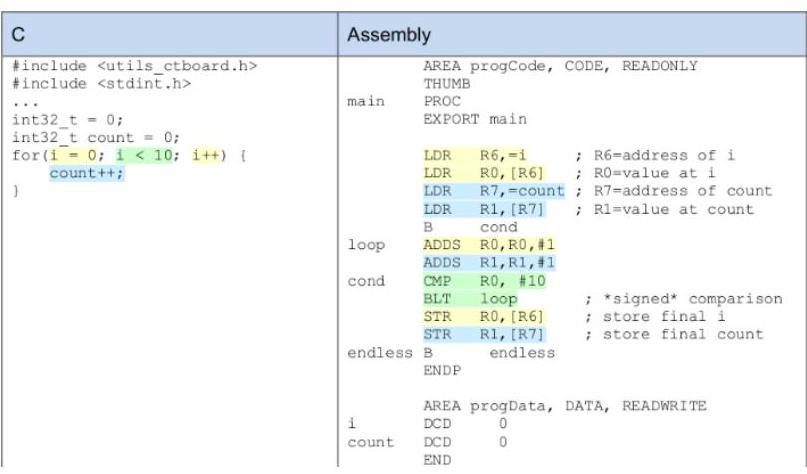
\includegraphics[width=\linewidth]{images/2024_12_29_79e6b22f503fb7b4f718g-07(2)}
\end{concept}

\begin{KR}{Implementing Control Structures}\\
Steps for implementing control structures:
\begin{enumerate}
  \item Choose appropriate control structure:
    \begin{itemize}
      \item If-then-else for simple decisions
      \item Switch for multiple cases with same variable
      \item Loops for repeated operations
    \end{itemize}
  \item For switches:
    \begin{itemize}
      \item Create jump table
      \item Calculate offset based on case value
      \item Handle default case
    \end{itemize}
  \item For loops:
    \begin{itemize}
      \item Initialize counter/condition
      \item Place condition check appropriately
      \item Ensure proper exit condition
      \item Update variables correctly
    \end{itemize}
\end{enumerate}
\end{KR}

\begin{example2}{Basic Control Structures}
Example implementations:
\begin{lstlisting}[language=armasm, style=basesmol]
    ; If-then-else
    CMP     R0, #0      ; Compare value
    BEQ     else_label  ; Branch if equal
    ; then code
    B       endif_label
else_label
    ; else code
endif_label

    ; While loop
    B       while_cond  ; Jump to condition
while_loop
    ; loop body
while_cond
    CMP     R0, #10     ; Check condition
    BLT     while_loop  ; Branch if less than

    ; Do-while loop
do_loop
    ; loop body
    CMP     R0, #10     ; Check condition
    BLT     do_loop     ; Branch if less than
\end{lstlisting}
\end{example2}

\begin{formula}{Branch Instruction Types}\\
Classification of branch instructions:

\textbf{1. Based on Condition:}
\begin{itemize}
  \item \textbf{Unconditional:}
    \begin{itemize}
      \item B - Branch always
      \item BL - Branch with Link
      \item BX - Branch and Exchange
    \end{itemize}
  \item \textbf{Conditional:}
    \begin{itemize}
      \item Flag-dependent (EQ, NE, CS, CC, etc.)
      \item Arithmetic (HI, LS, GE, LT, etc.)
    \end{itemize}
\end{itemize}

\textbf{2. Based on Target Address:}
\begin{itemize}
  \item \textbf{Direct:} Target address in instruction
  \item \textbf{Indirect:} Target address in register
  \item \textbf{Relative:} Offset from current PC
  \item \textbf{Absolute:} Complete target address
\end{itemize}
\end{formula}

\begin{KR}{Selection Implementation}\\
Guidelines for implementing if-then-else structures:

1. Simple if-then:
\begin{lstlisting}[language=armasm, style=basesmol]
    ; if (x > 0) { x++; }
    CMP     R0, #0          ; Compare x with 0
    BLE     endif           ; Skip if x <= 0
    ADDS    R0, #1          ; x++
endif
\end{lstlisting}

2. if-then-else:
\begin{lstlisting}[language=armasm, style=basesmol]
    ; if (x > y) { x = y; } else { y = x; }
    CMP     R0, R1          ; Compare x and y
    BLE     else_part       ; Branch if x <= y
    MOVS    R0, R1          ; Then part: x = y
    B       endif           ; Skip else part
else_part
    MOVS    R1, R0          ; Else part: y = x
endif
\end{lstlisting}

3. Nested if:
\begin{lstlisting}[language=armasm, style=basesmol]
    ; if (x > 0) {
    ;     if (y > 0) {
    ;         x = y;
    ;     }
    ; }
    CMP     R0, #0          ; Check x > 0
    BLE     endif_outer
    CMP     R1, #0          ; Check y > 0
    BLE     endif_inner
    MOVS    R0, R1          ; x = y
endif_inner
endif_outer
\end{lstlisting}
\end{KR}

\begin{KR}{Loop Implementation}\\
Templates for different loop types:

1. While loop:
\begin{lstlisting}[language=armasm, style=basesmol]
    ; while (x < 10) { x++; }
    B       while_cond      ; Jump to condition
while_loop
    ADDS    R0, #1          ; x++
while_cond
    CMP     R0, #10         ; Check x < 10
    BLT     while_loop      ; Continue if true
\end{lstlisting}

2. Do-while loop:
\begin{lstlisting}[language=armasm, style=basesmol]
    ; do { x++; } while (x < 10);
do_loop
    ADDS    R0, #1          ; x++
    CMP     R0, #10         ; Check x < 10
    BLT     do_loop         ; Continue if true
\end{lstlisting}

3. For loop:
\begin{lstlisting}[language=armasm, style=basesmol]
    ; for (i = 0; i < 10; i++)
    MOVS    R0, #0          ; i = 0
    B       for_cond
for_loop
    ; Loop body
    ADDS    R0, #1          ; i++
for_cond
    CMP     R0, #10         ; Check i < 10
    BLT     for_loop        ; Continue if true
\end{lstlisting}
\end{KR}

\begin{KR}{Switch Implementation}\\
Steps for implementing switch statements:

1. Range check and table access:
\begin{lstlisting}[language=armasm, style=basesmol]
    CMP     R0, #MAX_CASES  ; Check range
    BHS     default_case    ; If too high, default
    LSLS    R0, #2          ; Multiply by 4
    LDR     R1, =jump_table ; Load table address
    ADD     R1, R0          ; Add offset
    LDR     R1, [R1]        ; Load target address
    BX      R1              ; Branch to case
\end{lstlisting}

2. Jump table structure:
\begin{lstlisting}[language=armasm, style=basesmol]
jump_table
    DCD     case_0          ; Case 0 handler
    DCD     case_1          ; Case 1 handler
    DCD     default_case    ; Default handler
    ; ... more cases
\end{lstlisting}

3. Case handlers:
\begin{lstlisting}[language=armasm, style=basesmol]
case_0
    ; Handle case 0
    B       switch_end
case_1
    ; Handle case 1
    B       switch_end
default_case
    ; Handle default case
switch_end
\end{lstlisting}
\end{KR}

\begin{example2}{Complex Control Structure}
Implementing nested loops with conditions:
\begin{lstlisting}[language=armasm, style=basesmol]
    ; for (i = 0; i < 5; i++) {
    ;     if (i == 2) continue;
    ;     for (j = 0; j < 3; j++) {
    ;         if (j == 1) break;
    ;         sum += i + j;
    ;     }
    ; }
    
    MOVS    R0, #0          ; i = 0
outer_loop
    CMP     R0, #2          ; Check i == 2
    BEQ     outer_continue  ; Skip if i == 2
    
    MOVS    R1, #0          ; j = 0
inner_loop
    CMP     R1, #1          ; Check j == 1
    BEQ     outer_continue  ; Break to outer loop
    
    ADDS    R2, R0, R1      ; Calculate i + j
    ADDS    R4, R4, R2      ; Add to sum
    
    ADDS    R1, #1          ; j++
    CMP     R1, #3          ; Check j < 3
    BLT     inner_loop      ; Continue inner loop
    
outer_continue
    ADDS    R0, #1          ; i++
    CMP     R0, #5          ; Check i < 5
    BLT     outer_loop      ; Continue outer loop
\end{lstlisting}
\end{example2}


	\raggedcolumns
	\subsection{Examples}

\begin{concept}{Branch Types Overview}\\
Three main classifications of branches:

\textbf{By Condition:}
\begin{itemize}
  \item \textbf{Unconditional}: Branch always
  \item \textbf{Conditional}: Branch only if condition is met
\end{itemize}

\textbf{By Target Address:}
\begin{itemize}
  \item \textbf{Relative}: Target address relative to PC
  \item \textbf{Absolute}: Complete target address
\end{itemize}

\textbf{By Address Hand-over:}
\begin{itemize}
  \item \textbf{Direct}: Target address part of instruction
  \item \textbf{Indirect}: Target address in register
\end{itemize}

%\includegraphics[width=\linewidth]{images/branch_overview.png}
\end{concept}

\begin{example2}{Unconditional Branch Flow}\\
Example of branching sequence and jump table:
\begin{lstlisting}[language=armasm, style=basesmol]
Label1  LDR     R0, =Label5
Label2  BX      R0
Jumptable
        DCD     Case0
        DCD     Case1
        DCD     Case2
        DCD     Case3
Label5  LDR     R0, =Label6
        B       Label2
Label6  LDR     R2, =Jumptable
        ADDS    R2, R2, #4
Label4  LDR     R2, [R2]
        BX      R2
Case0   B       Case0           ; Infinite loop
Case1   B       Label1
Case2   B       Label1
Case3   B       Case0
\end{lstlisting}
\end{example2}

\begin{KR}{Branch Pattern Recognition}\\
Common branch patterns and their uses:

1. Basic branching:
\begin{lstlisting}[language=armasm, style=basesmol]
    ; Simple jump
    B       target          ; Unconditional
    BEQ     target          ; Branch if equal
    BNE     target          ; Branch if not equal
    
    ; Conditional execution
    CMP     R0, #value
    BCC     target          ; Branch if carry clear
    BGT     target          ; Branch if greater than
\end{lstlisting}

2. Jump tables:
\begin{lstlisting}[language=armasm, style=basesmol]
    ; Load table base
    LDR     R0, =jumptable
    ; Calculate offset
    LSLS    R1, R1, #2      ; Multiply index by 4
    ADDS    R0, R0, R1      ; Add to base
    ; Jump to handler
    LDR     R0, [R0]        ; Load address
    BX      R0              ; Branch to handler
\end{lstlisting}

3. Infinite loops:
\begin{lstlisting}[language=armasm, style=basesmol]
endless B       endless      ; Simple infinite loop

loop    ; Do something
        B       loop        ; Loop forever
\end{lstlisting}
\end{KR}

\begin{example2}{Conditional Branches with Flag Testing}\\
Example tracking non-taken branches:
\begin{lstlisting}[language=armasm, style=basesmol]
    MOVS    R0, #0          ; Clear mask
    
    ; Test carry flag
    ADDS    R1, R1, #5
    BCS     taken
    ADDS    R0, R0, #0x01   ; Mark if not taken
taken

    ; Test equality
    ANDS    R1, R1, R5
    BEQ     equal
    ADDS    R0, R0, #0x02   ; Mark if not taken
equal

    ; Test overflow
    SUBS    R2, R2, R5
    BVS     overflow
    ADDS    R0, R0, #0x04   ; Mark if not taken
overflow
\end{lstlisting}

Result in R0 shows which branches were not taken.
\end{example2}

\begin{example2}{Comparison Instructions}\\
Using CMP and TST instructions:
\begin{lstlisting}[language=armasm, style=basesmol]
    ; Signed comparisons
    LDR     R1, =0xFFFFFFFF
    CMP     R1, #1          ; Compare with immediate
    BLT     is_less         ; Branch if less than
    
    ; Unsigned comparisons
    CMP     R1, #1
    BLO     is_below        ; Branch if lower
    
    ; Bit testing
    LDR     R5, =0x0040FFFF
    TST     R3, R5          ; Test bits
    BNE     bits_set        ; Branch if any bit set
    BEQ     bits_clear      ; Branch if all bits clear
\end{lstlisting}
\end{example2}

\begin{KR}{Flow Control Implementation}\\
Guidelines for implementing control structures:

1. If-Then-Else:
\begin{lstlisting}[language=armasm, style=basesmol]
    ; if (condition) {
    ;     then-part
    ; } else {
    ;     else-part
    ; }
    CMP     R0, #value      ; Test condition
    BNE     else_part       ; Branch if false
then_part
    ; Then code
    B       endif           ; Skip else
else_part
    ; Else code
endif
\end{lstlisting}

2. Switch-Case:
\begin{lstlisting}[language=armasm, style=basesmol]
    ; switch(value) {
    ;    case 0: ... break;
    ;    case 1: ... break;
    ; }
    LDR     R0, =jumptable
    LSLS    R1, R1, #2      ; Index * 4
    ADD     R0, R1          ; Add to base
    LDR     R0, [R0]        ; Get handler
    BX      R0              ; Jump to handler

jumptable
    DCD     case0
    DCD     case1
\end{lstlisting}

3. Loops:
\begin{lstlisting}[language=armasm, style=basesmol]
    ; while (condition) {
    ;     body
    ; }
    B       test            ; Jump to test
loop
    ; Loop body
test
    CMP     R0, #value      ; Test condition
    BLT     loop           ; Continue if true
\end{lstlisting}
\end{KR}

\begin{remark}
Important considerations:
\begin{itemize}
  \item Consider branch range limitations
  \item Be aware of condition flag changes
  \item Handle corner cases in comparisons
  \item Plan for proper loop termination
  \item Document complex branching logic
\end{itemize}
\end{remark}

\section*{CT1 Exercises for Branching Instructions}
\section*{Content}
CT1 Exercises for Branching Instructions ..... 1\\
Exercise 1 - Unconditional Branches ..... 2\\
Exercise 2 - Conditional Branches ..... 3\\
Exercise 3 - Comparison Instructions ..... 4\\
Solutions ..... 5\\
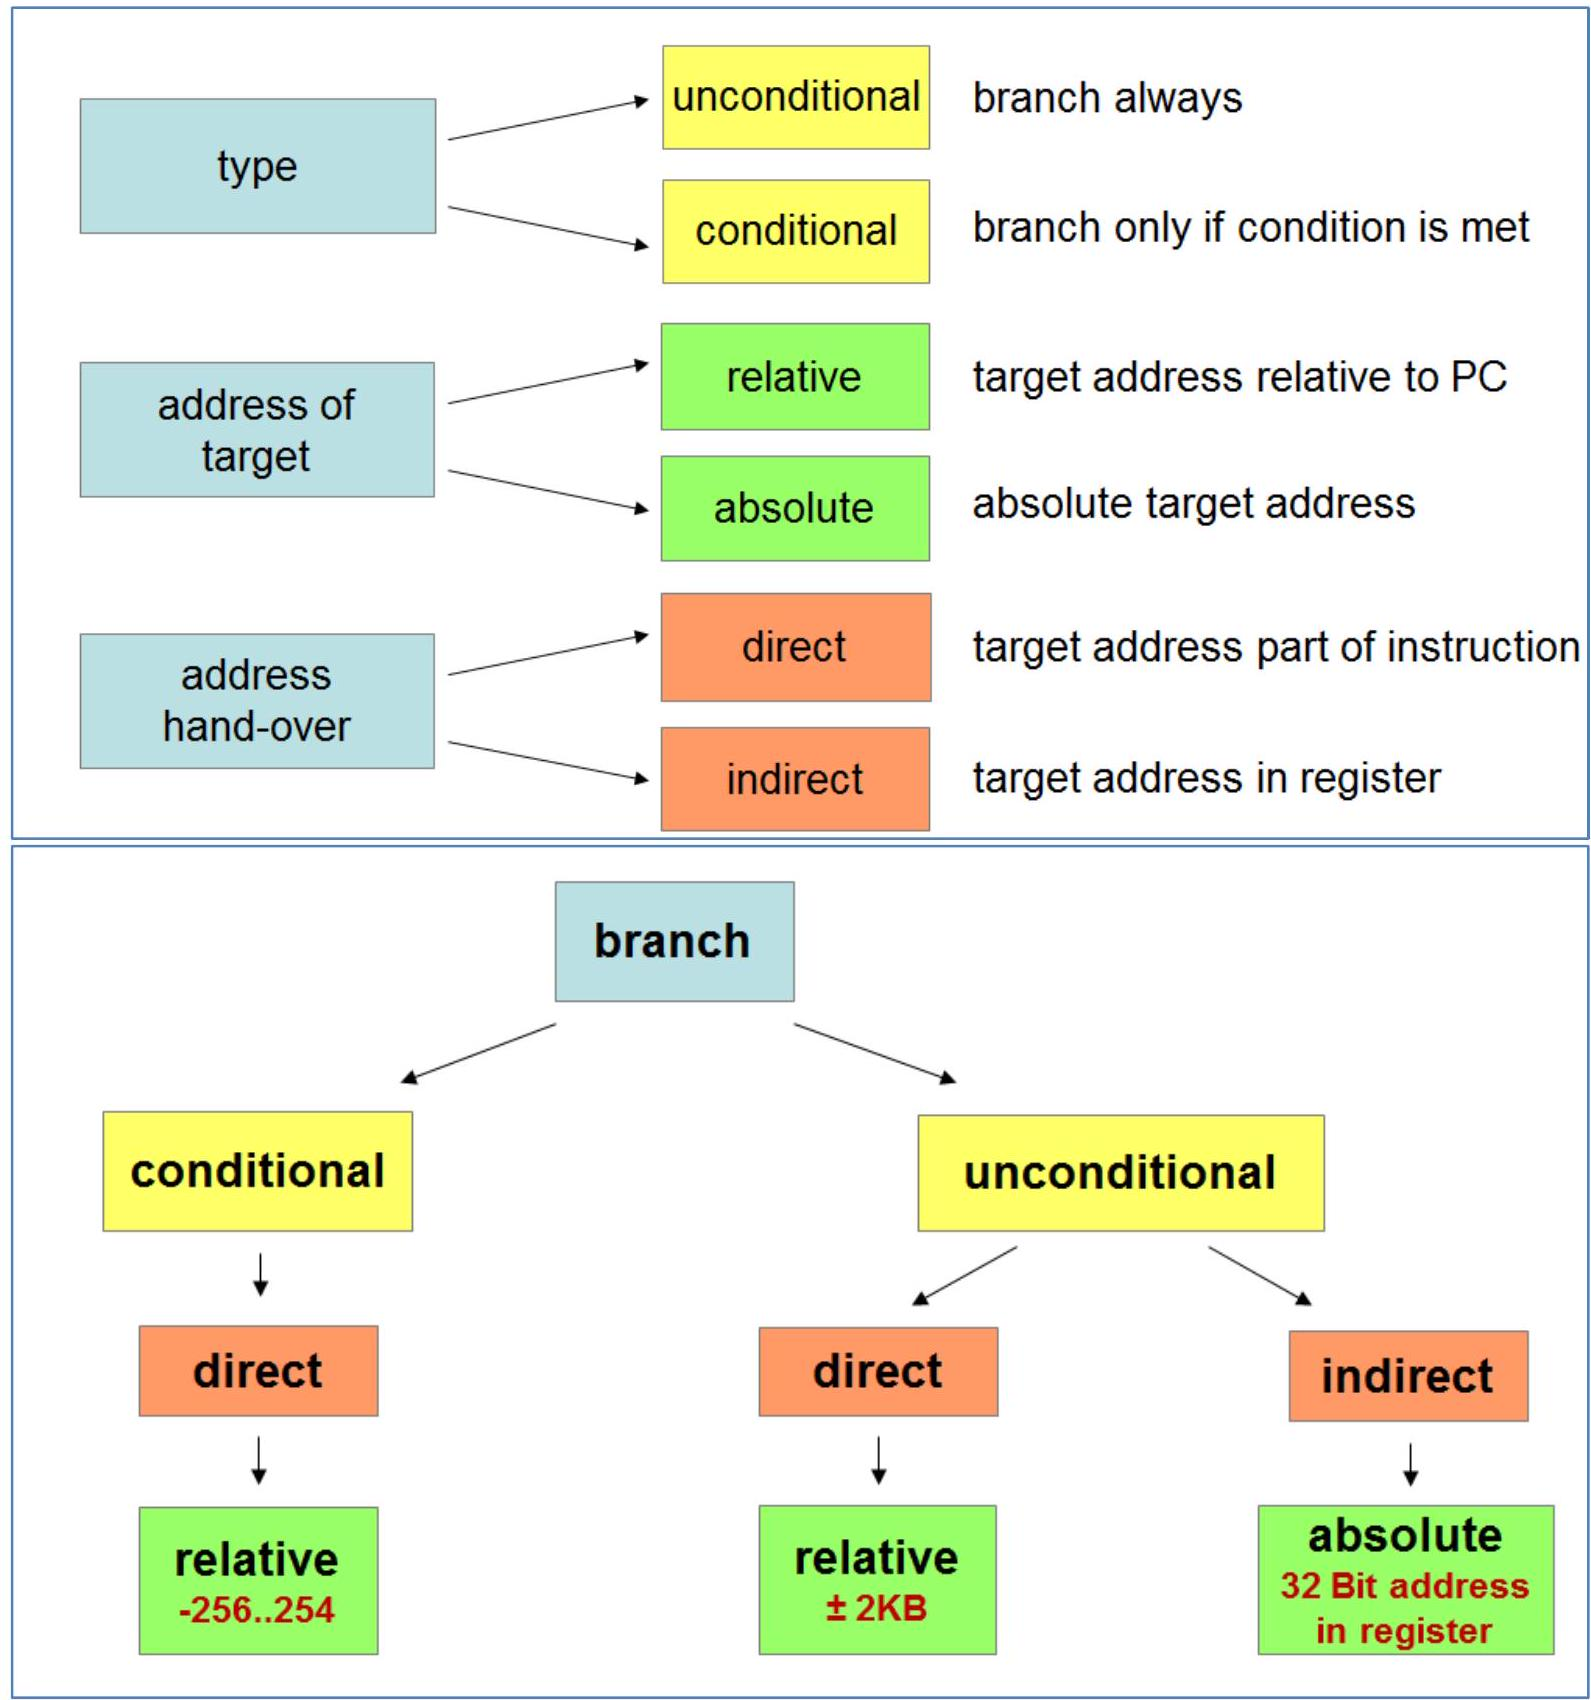
\includegraphics[width=\linewidth]{images/2025_01_02_9902c2d2685de638ef73g-1}

\section*{Exercise 1 - Unconditional Branches}
The execution starts at line 10.

\begin{enumerate}
  \item List the sequence of branch instructions that end in an infinite loop.
\end{enumerate}

Do this by stating the branches in tabular form: from - to.\\
E.g. the first branch is $\underline{\mathbf{1 1 - 1 6}}$ (branch unconditionally from line 11 to line 16).\\
2) At which line does the execution sequence finally loop forever?

\begin{center}
\begin{tabular}{|l|lll|}
\hline
10 & Label1 & LDR & R0, =Label5 \\
11 & Label2 & BX & R0 \\
12 & Jumptable & DCD & Case0 \\
13 &  & DCD & Case1 \\
14 &  & DCD & Case2 \\
15 &  & DCD & Case3 \\
16 & Label5 & LDR & R0, =Label6 \\
17 &  & B & Label2 \\
18 & Label6 & LDR & R2, =Jumptable \\
19 &  & ADDS R2, R2, \#4 &  \\
20 & Label4 & LDR R2, [R2] &  \\
21 &  & BX & R2 \\
22 & Case0 & B & Case0 \\
23 & Case1 & LDR & R2, =Jumptable \\
24 &  & MOVS R1, \#3 &  \\
25 &  & LSLS R1, R1, \#2 &  \\
26 &  & ADDS R2, R2, R1 &  \\
27 &  & B & Label4 \\
28 & Case2 & B & Label1 \\
29 & Case3 & B & Case0 \\
\hline
\end{tabular}
\end{center}

Your solution (the number of cells below is no hint)\\
1)

\begin{center}
\begin{tabular}{|l|l|l|l|l|l|l|l|}
\hline
$11-16$ &  &  &  &  &  &  &  \\
\hline
\end{tabular}
\end{center}

2.

\section*{Exercise 2 - Conditional Branches}
The execution starts at line 10.

\begin{enumerate}
  \item List which branch instructions jump to the given label.
\end{enumerate}

Do this by stating the branches in tabular form: from - to.\\
2) What is the final value in $R 0$ as hexadecimal value?\\
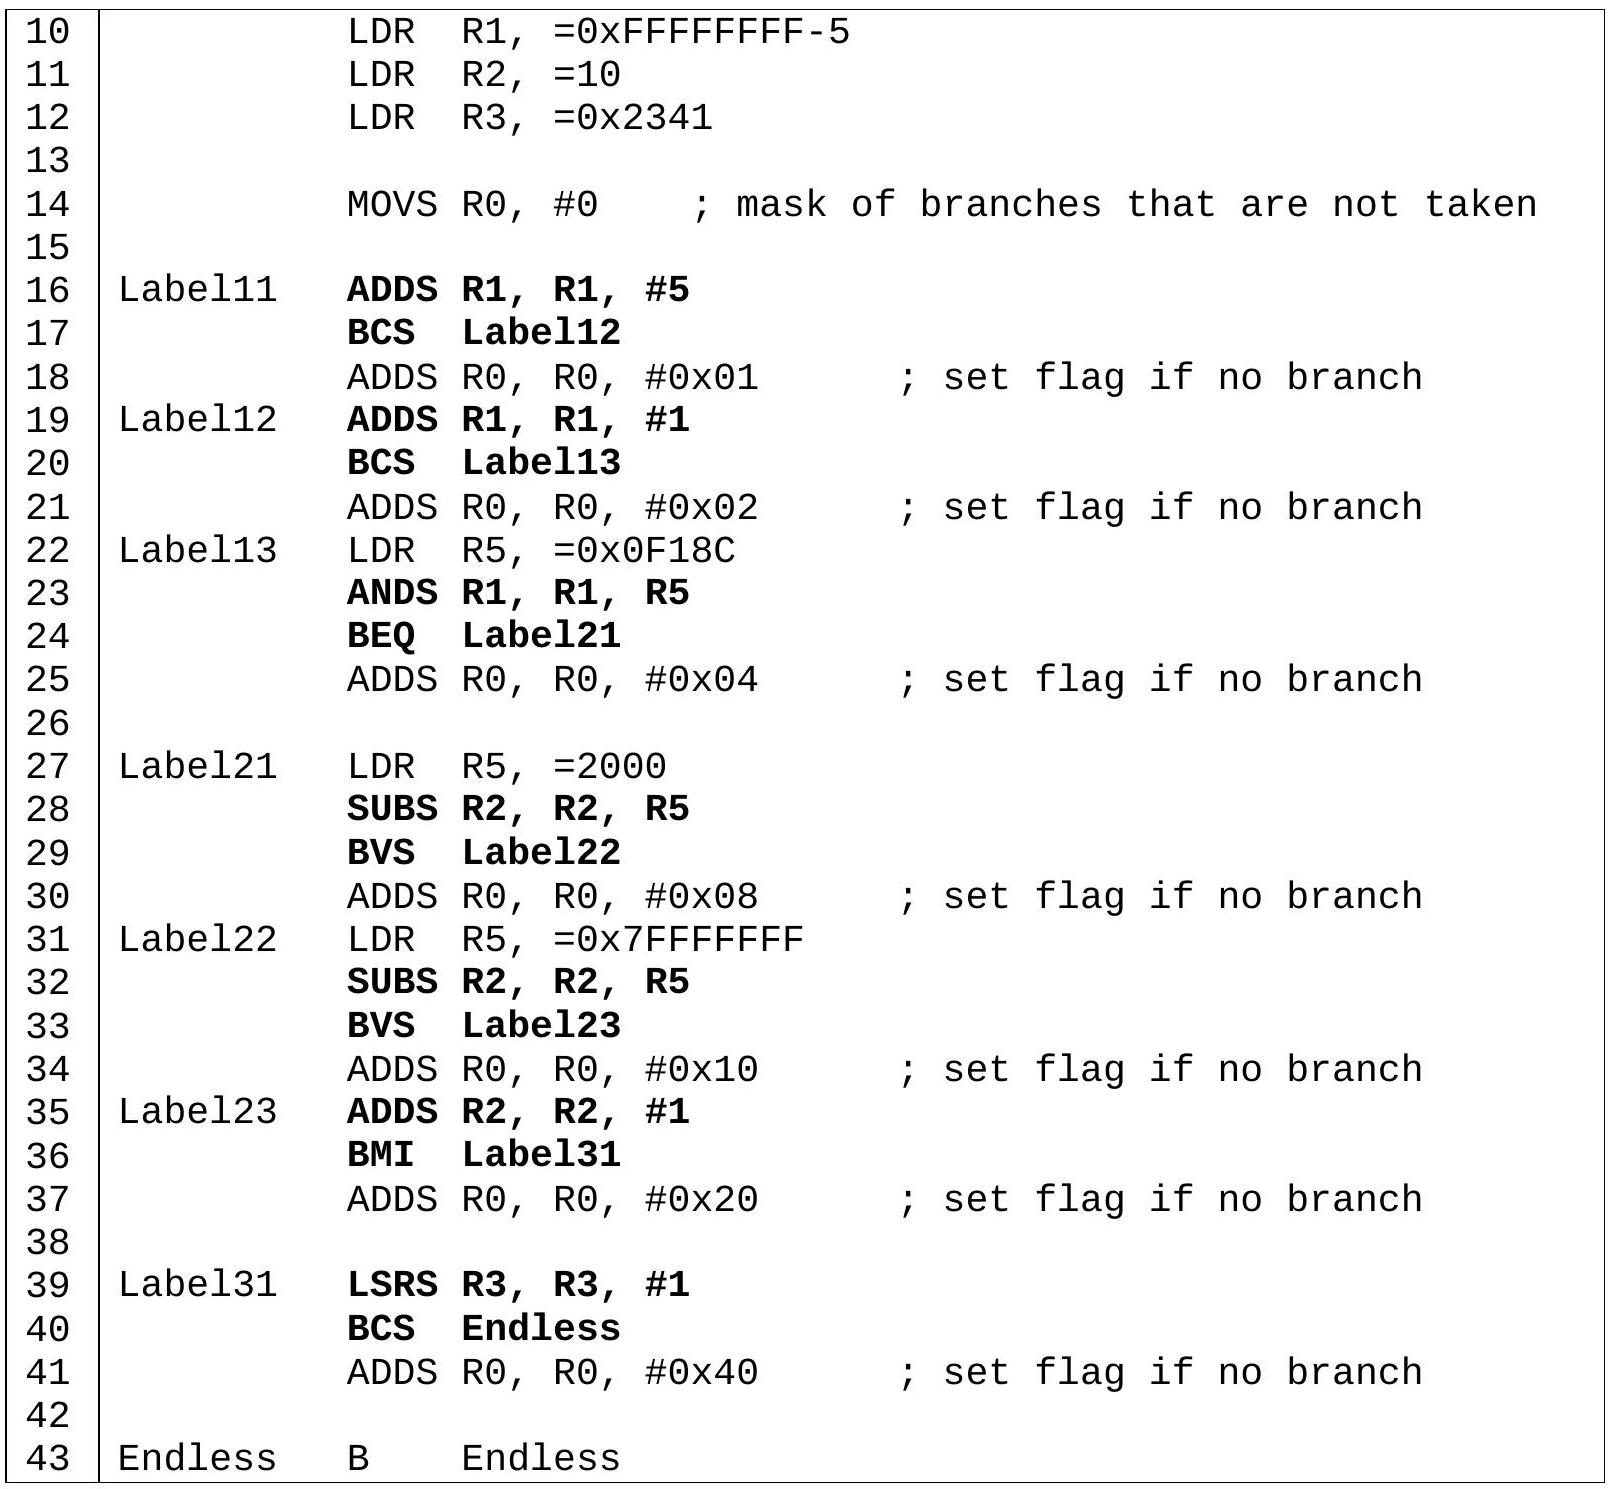
\includegraphics[width=\linewidth]{images/2025_01_02_9902c2d2685de638ef73g-3}

Your solution (the number of cells below is no hint)

\begin{enumerate}
  \item $\square$
  \item $\quad R 0=0 x$. $\qquad$
\end{enumerate}

\section*{Exercise 3 - Comparison Instructions}
The execution starts at line 10.

\begin{enumerate}
  \item List which branch instructions jump to the given label.
\end{enumerate}

Do this by stating the branches in tabular form: from - to.\\
2) What is the final value in $R 0$ as hexadecimal value?\\
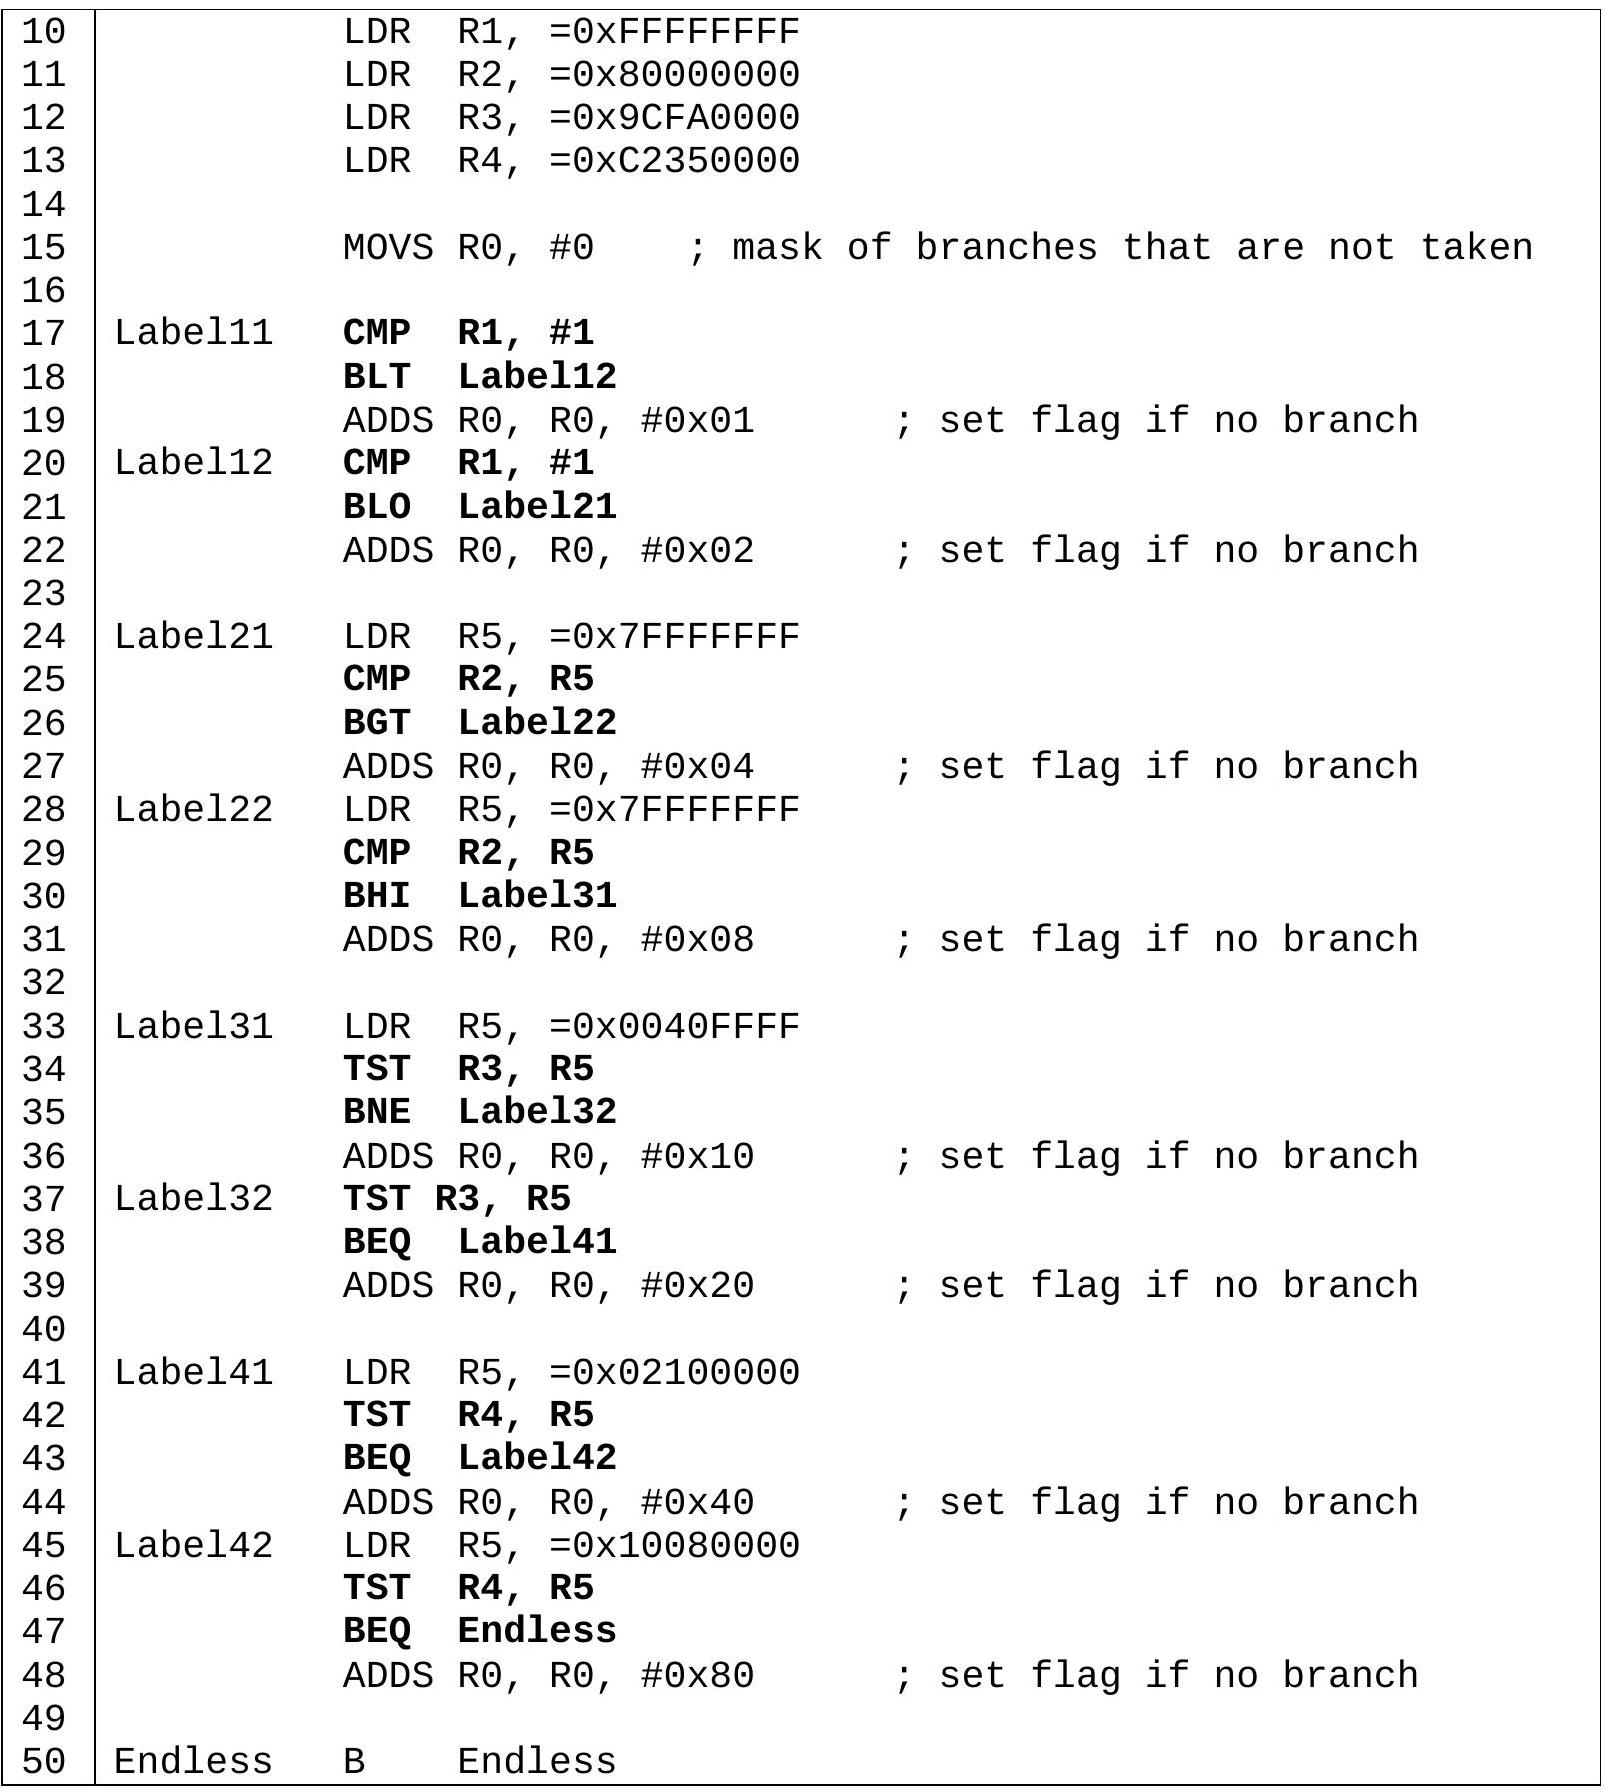
\includegraphics[width=\linewidth]{images/2025_01_02_9902c2d2685de638ef73g-4}

Your solution (the number of cells below is no hint)

\begin{enumerate}
  \item $\square$
  \item $\quad R O=0 x$. $\qquad$
\end{enumerate}

\section*{Solutions}
\section*{Exercise 1:}
\begin{enumerate}
  \item $10-16,17-11,11-18,21-23,27-20,21-29,29-22,22-22 \ldots$
  \item Loops at line 22
\end{enumerate}

\section*{Exercise 2:}
\begin{enumerate}
  \item $20-22,24-27,33-35,40-43$
  \item $0 \times 29$ (binary 0010 '1001)
\end{enumerate}

\section*{Exercise 3:}
\begin{enumerate}
  \item $18-20,30-33,35-37,47-50$
  \item $0 \times 66$ (binary 0110 '0110)
\end{enumerate}

\subsection{Examples}

\begin{concept}{Control Structure Types}\\
Three fundamental types of control structures:

\textbf{1. Sequence}:
\begin{itemize}
  \item Linear execution of instructions
  \item No branching or decisions
  \item Operations performed in order
\end{itemize}

\textbf{2. Selection}:
\begin{itemize}
  \item Conditional execution (if-then-else)
  \item Branch based on condition
  \item Different paths based on test
\end{itemize}

\textbf{3. Iteration}:
\begin{itemize}
  \item Repeated execution (loops)
  \item Condition-controlled repetition
  \item Fixed number of repetitions
\end{itemize}

%\includegraphics[width=\linewidth]{images/control_structures_overview.png}
\end{concept}

\begin{example2}{Selection Structures}\\
If-Then-Else with unsigned 8-bit variables:

\begin{lstlisting}[language=C, style=basesmol]
// C code
uint8_t nrX = ...;
uint8_t nrY = ...;
if (nrX > nrY) {
    nrX = nrY;
} else {
    nrY = nrX;
}
\end{lstlisting}

Assembly implementation:
\begin{lstlisting}[language=armasm, style=basesmol]
    AREA    progCode, CODE, READONLY
    THUMB
main
    PROC
    EXPORT  main
    
    LDR     R6, =nrX      ; R6 = address of nrX
    LDRB    R0, [R6]      ; R0 = byte stored at nrX
    LDR     R7, =nrY      ; R7 = address of nrY
    LDRB    R1, [R7]      ; R1 = byte stored at nrY
    CMP     R0, R1
    BLS     else          ; *unsigned* comparison
    STRB    R1, [R6]      ; store nrY value at nrX
    B       endif
else
    STRB    R0, [R7]      ; store nrX value at nrY
endif
    ENDP
\end{lstlisting}
\end{example2}

\begin{KR}{Selection Implementation}\\
Guidelines for implementing if-then-else structures:

1. Single condition:
\begin{lstlisting}[language=armasm, style=basesmol]
    ; if (condition) {
    ;     then-part
    ; } else {
    ;     else-part
    ; }
    
    ; Test condition
    CMP     Rx, Ry            ; Compare values
    B<cc>   else_label        ; Branch if condition false
    
    ; Then part
    <then instructions>
    B       endif_label       ; Skip else part
    
else_label
    ; Else part
    <else instructions>
    
endif_label
    ; Continue execution
\end{lstlisting}

2. Multiple conditions (AND):
\begin{lstlisting}[language=armasm, style=basesmol]
    ; if (condA && condB) {
    ;     then-part
    ; } else {
    ;     else-part
    ; }
    
    ; Test first condition
    CMP     Rx, #valA
    B<cc>   else_label        ; Branch if first fails
    
    ; Test second condition
    CMP     Ry, #valB
    B<cc>   else_label        ; Branch if second fails
    
    ; Then part
    <then instructions>
    B       endif_label
    
else_label
    ; Else part
    <else instructions>
    
endif_label
\end{lstlisting}

3. Multiple conditions (OR):
\begin{lstlisting}[language=armasm, style=basesmol]
    ; if (condA || condB) {
    ;     then-part
    ; } else {
    ;     else-part
    ; }
    
    ; Test first condition
    CMP     Rx, #valA
    B<cc>   test_second       ; Try second if first fails
    B       then_label        ; First succeeded
    
test_second
    CMP     Ry, #valB
    B<cc>   else_label        ; Branch if both fail
    
then_label
    ; Then part
    <then instructions>
    B       endif_label
    
else_label
    ; Else part
    <else instructions>
    
endif_label
\end{lstlisting}
\end{KR}

\begin{example2}{For-Loop Implementation}\\
Example for-loop in C and assembly:

\begin{lstlisting}[language=C, style=basesmol]
// C code with volatile variables
volatile int32_t i = 0;
volatile int32_t count = 0;
for(i = 0; i < 10; i++) {
    count++;
}
\end{lstlisting}

Assembly implementation:
\begin{lstlisting}[language=armasm, style=basesmol]
    AREA    progCode, CODE, READONLY
    THUMB
main
    PROC
    EXPORT  main
    
    LDR     R6, =i          ; R6 = address of i
    LDR     R0, [R6]        ; R0 = value at i
    LDR     R7, =count      ; R7 = address of count
    LDR     R1, [R7]        ; R1 = value at count
    B       cond
    
loop
    ADDS    R0, R0, #1      ; Increment i
    ADDS    R1, R1, #1      ; Increment count
cond
    CMP     R0, #10
    BLT     loop            ; Branch if i < 10
    
    STR     R0, [R6]        ; Store final i
    STR     R1, [R7]        ; Store final count
    ENDP
\end{lstlisting}

Compiler-optimized version:
\begin{lstlisting}[language=armasm, style=basesmol]
    LDR     r1, [pc, #20]   ; Load address
    MOVS    r0, #0          ; Initialize counter
    STR     r0, [r1, #0]    ; Store i
    LDR     r2, [r1, #4]    ; Load count
    
increment
    ADDS    r0, r0, #1      ; i++
    ADDS    r2, r2, #1      ; count++
    CMP     r0, #10         ; Check condition
    BLT     increment       ; Loop if i < 10
    STM     r1!, {r0, r2}   ; Store final values
\end{lstlisting}
\end{example2}

\begin{example2}{String Processing Loop}\\
Converting string to uppercase:
\begin{lstlisting}[language=armasm, style=basesmol]
    AREA    progCode, CODE, READONLY
    THUMB
main
    PROC
    EXPORT  main
    LDR     R0, =srcstr     ; Source string
    LDR     R1, =outstr     ; Output string
    MOVS    R2, #0          ; Initialize index
    
cond
    LDRB    R3, [R0, R2]    ; Load character
    CMP     R3, #0          ; Check for end
    BEQ     endloop         ; Exit if done
    CMP     R3, #60         ; Check if < 'a'
    BLO     store           ; Skip if not lowercase
    CMP     R3, #90         ; Check if > 'z'
    BHI     store           ; Skip if not lowercase
    ADDS    R3, R3, #32     ; Convert to uppercase
    
store
    STRB    R3, [R1, R2]    ; Store character
    ADDS    R2, R2, #1      ; Next character
    B       cond            ; Continue loop
    
endloop
    STRB    R3, [R1, R2]    ; Store terminator
    ENDP
    
srcstr  DCB     "This IS mY TestStriNG", 0
    AREA    progData, DATA, READWRITE
outstr  SPACE   50
\end{lstlisting}

Result: "THIS IS MY TESTSTRING"
\end{example2}

\begin{KR}{String Processing Patterns}\\
Common patterns for string manipulation:

1. String traversal:
\begin{lstlisting}[language=armasm, style=basesmol]
    MOVS    R2, #0          ; Index
loop
    LDRB    R3, [R0, R2]    ; Load char
    CMP     R3, #0          ; Check end
    BEQ     done            ; Exit if terminator
    ; Process character
    ADDS    R2, R2, #1      ; Next char
    B       loop
\end{lstlisting}

2. Character transformation:
\begin{lstlisting}[language=armasm, style=basesmol]
    ; Check character range
    CMP     R3, #lower_bound
    BLO     skip            ; Below range
    CMP     R3, #upper_bound
    BHI     skip            ; Above range
    
    ; Transform character
    ADDS    R3, #offset     ; Apply offset
    
skip
    STRB    R3, [R1, R2]    ; Store result
\end{lstlisting}

3. String copy:
\begin{lstlisting}[language=armasm, style=basesmol]
    MOVS    R2, #0          ; Index
copy_loop
    LDRB    R3, [R0, R2]    ; Load source
    STRB    R3, [R1, R2]    ; Store to dest
    ADDS    R2, R2, #1      ; Next char
    CMP     R3, #0          ; Check end
    BNE     copy_loop       ; Continue if not done
\end{lstlisting}
\end{KR}

\begin{remark}
Important considerations:
\begin{itemize}
  \item Choose appropriate conditional branches
  \item Consider signed vs unsigned comparisons
  \item Handle edge cases and termination
  \item Maintain proper register allocation
  \item Document complex control flow
\end{itemize}
\end{remark}

\section*{CT1 Exercises for Control Structures}
\section*{Content}
CT1 Exercises for Control Structures ..... 1\\
Exercise 1 - Selection/Branch ..... 2\\
Exercise 2 - For-Loops ..... 3\\
Exercise 3 - From Code to Structogram ..... 4\\
Solutions ..... 5

\section*{Exercise 1 - Selection/Branch}
Encode the following Structograms into Flowchart, C- and ARM Assembly-language\\
A) If-Then-Else with unsigned 8-bit variables

\begin{center}
\begin{tabular}{|c|c|}
\hline
$n r X=n r Y$ & else \\
\hline
then $(n r X>n r Y)$ &  \\
\hline
\end{tabular}
\end{center}

B) If-Then-Else with signed 8-bit variables

\begin{center}
\begin{tabular}{|c|c|c|}
\hline
\multicolumn{3}{|l|}{\(
\text { then } \quad \text { if }(\operatorname{varA}<-17 \text { AND }
\)} \\
\hline
$\operatorname{varA}=-\operatorname{varB}$ &  & varB \\
\hline
\end{tabular}
\end{center}

C) If-Then-Else with signed 16-bit variables

\begin{comment}
\begin{center}
\begin{tabular}{|c|c|}
\hline
 & \multicolumn{3}{|c|}{\begin{tabular}{l}
if $(\operatorname{varC}=2344$ OR \\
$\operatorname{varC}>6788)$ \\
\end{tabular}} \\
\hline
then & else &  &  \\
\hline
$\operatorname{varC}=\operatorname{varC} / 4$ & $\operatorname{varC}=\operatorname{varC} / 2$ &  &  \\
\hline
\end{tabular}
\end{center}
\end{comment}

\section*{Exercise 2 - For-Loops}
A) Write a for-loop in C- and ARM Assembly-language.\\
B) Compare your Assembly-language implementation with the compiler generated one. Hint: In the Keil uVision5 IDE

\begin{enumerate}
  \item create an empty C-language project (according to the respective introduction documents)
  \item add the C-language for-loop to the empty main function
  \item compile the project
  \item set a breakpoint in at the first line of the main function
  \item start debugging the program and let it run into the breakpoint
  \item compare your Assembly-language implementation of the for-loop with the compiler generated one
\end{enumerate}

Hint: for the purpose of this exercise, define your variables global and as "volatile" this tells the compiler to not optimize away the access to the variables since they are not used otherwise.

\section*{Exercise 3 - From Code to Structogram}
A) Analyze the following Assembly-language code and derive from this the matching structogram.\\
B) What result is stored in "outstr"?

\begin{verbatim}
    AREA progCode, CODE, READONLY
    THUMB
main
    PROC
    EXPORT main
    LDR R0,=srcstr
    LDR R1,=outstr
    MOVS R2,#0
cond LDRB R3,[R0,R2]
    CMP R3,#0
    BEQ endloop
    CMP R3,#60
    BLO store
    CMP R3,#90
    BHI store
    ADDS R3,R3,#32
store STRB R3,[R1,R2]
    ADDS R2,R2,#1
    B cond
endloop STRB R3,[R1,R2]
endless B endless
srcstr DCB "This IS mY TestStriNG", 0
    AREA progData, DATA, READWRITE
outstr SPACE 50
    END
\end{verbatim}

\section*{Solutions}
\section*{Exercise 1:}
A) If-Then-Else with unsigned 8-bit variables\\
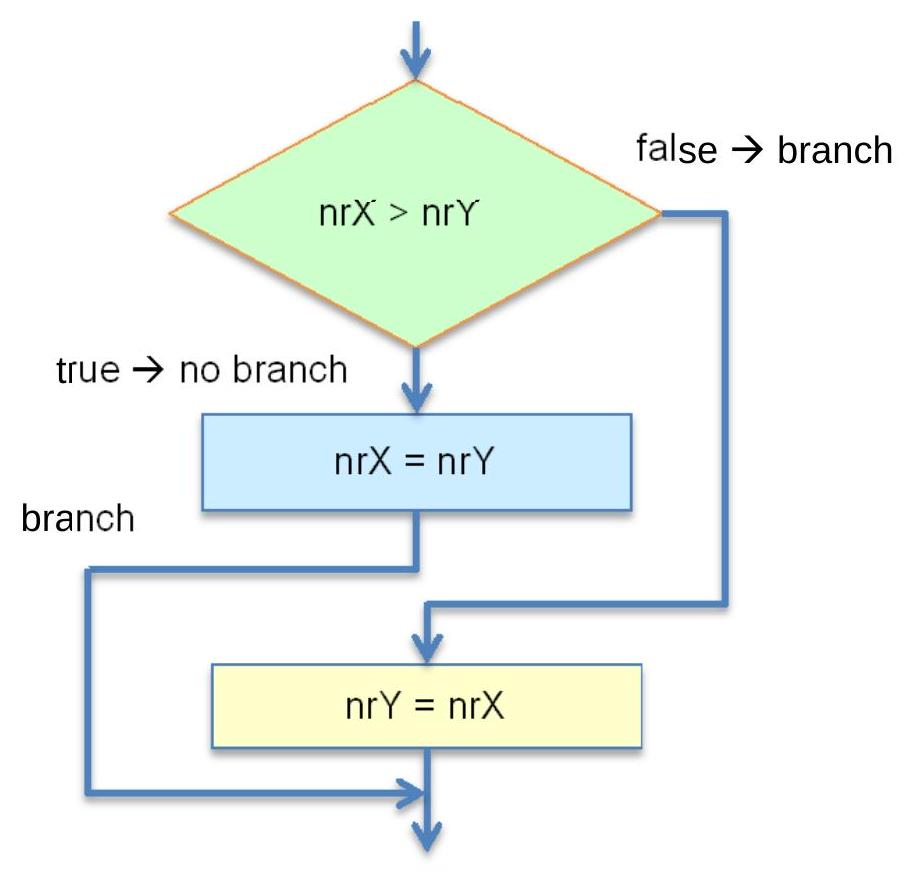
\includegraphics[width=\linewidth]{images/2025_01_02_7eee2d56b23c0199f878g-5}\\
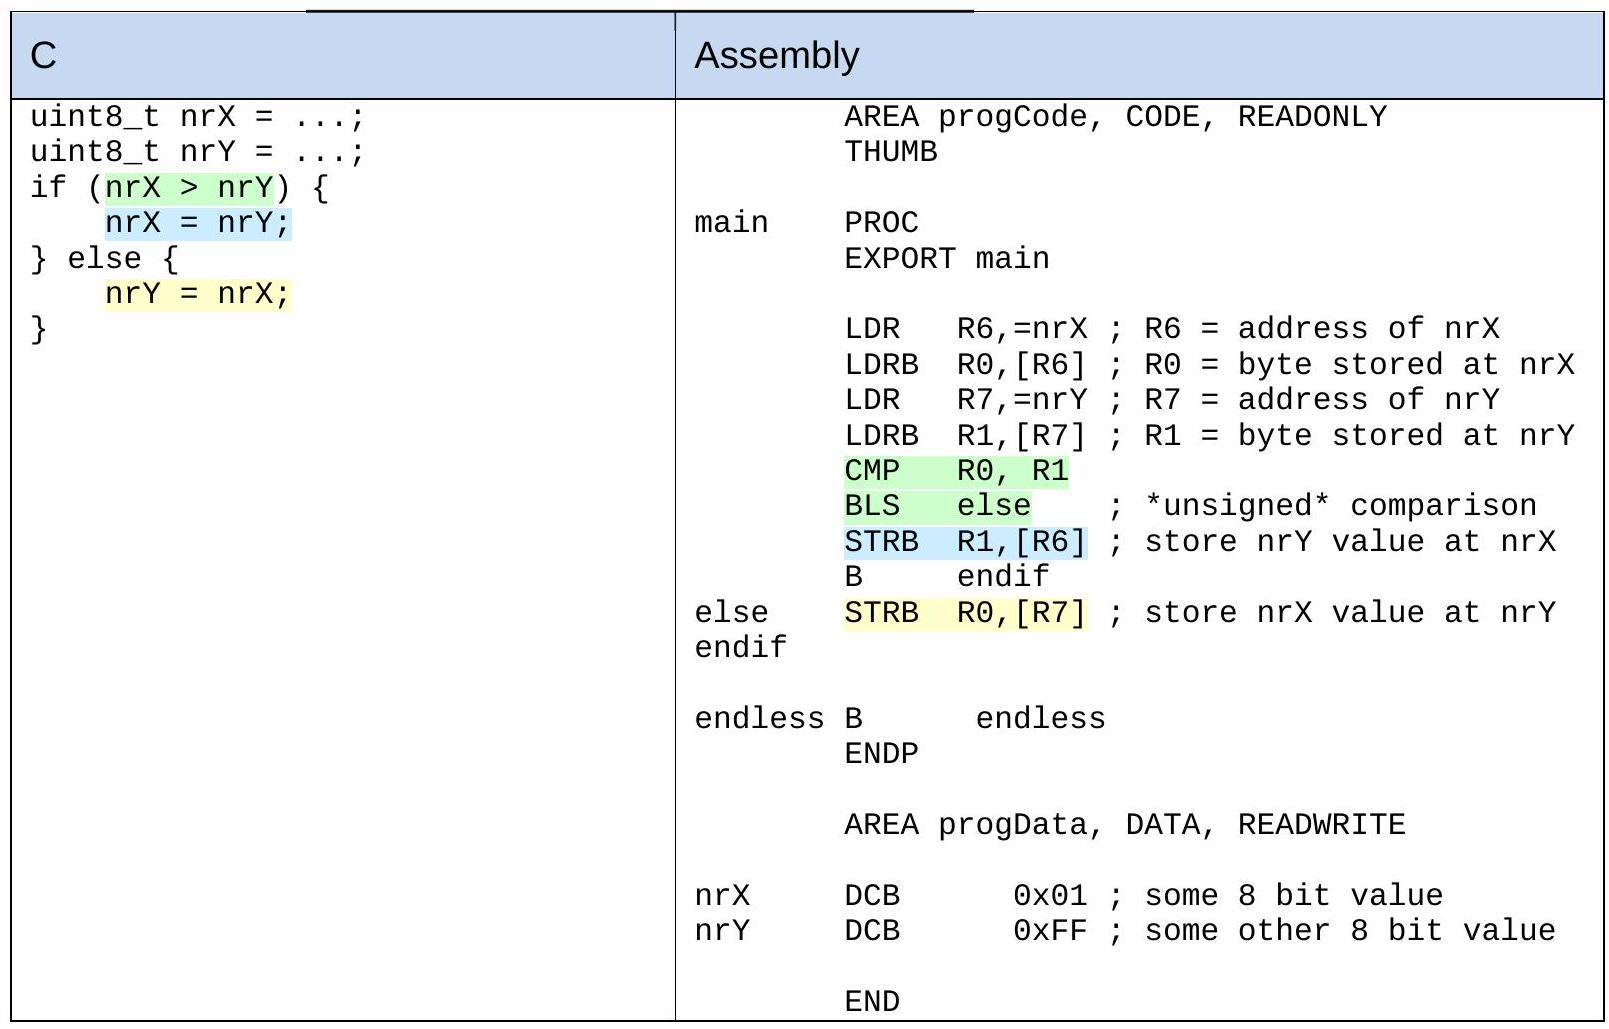
\includegraphics[width=\linewidth]{images/2025_01_02_7eee2d56b23c0199f878g-5(1)}\\
B) If-Then-Else with signed 8-bit variables\\
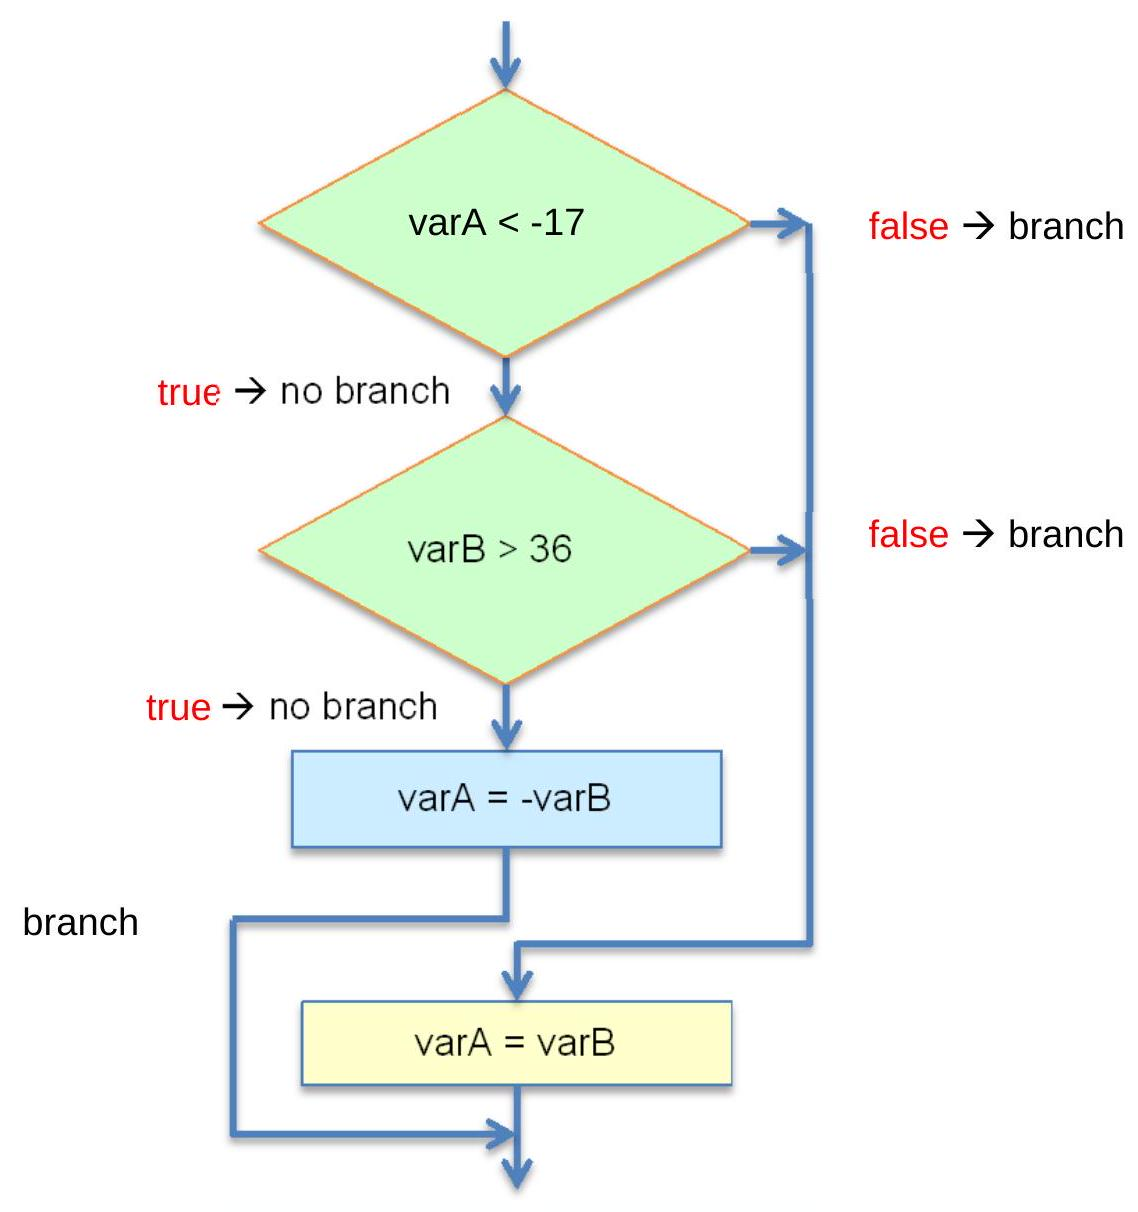
\includegraphics[width=\linewidth]{images/2025_01_02_7eee2d56b23c0199f878g-6}\\
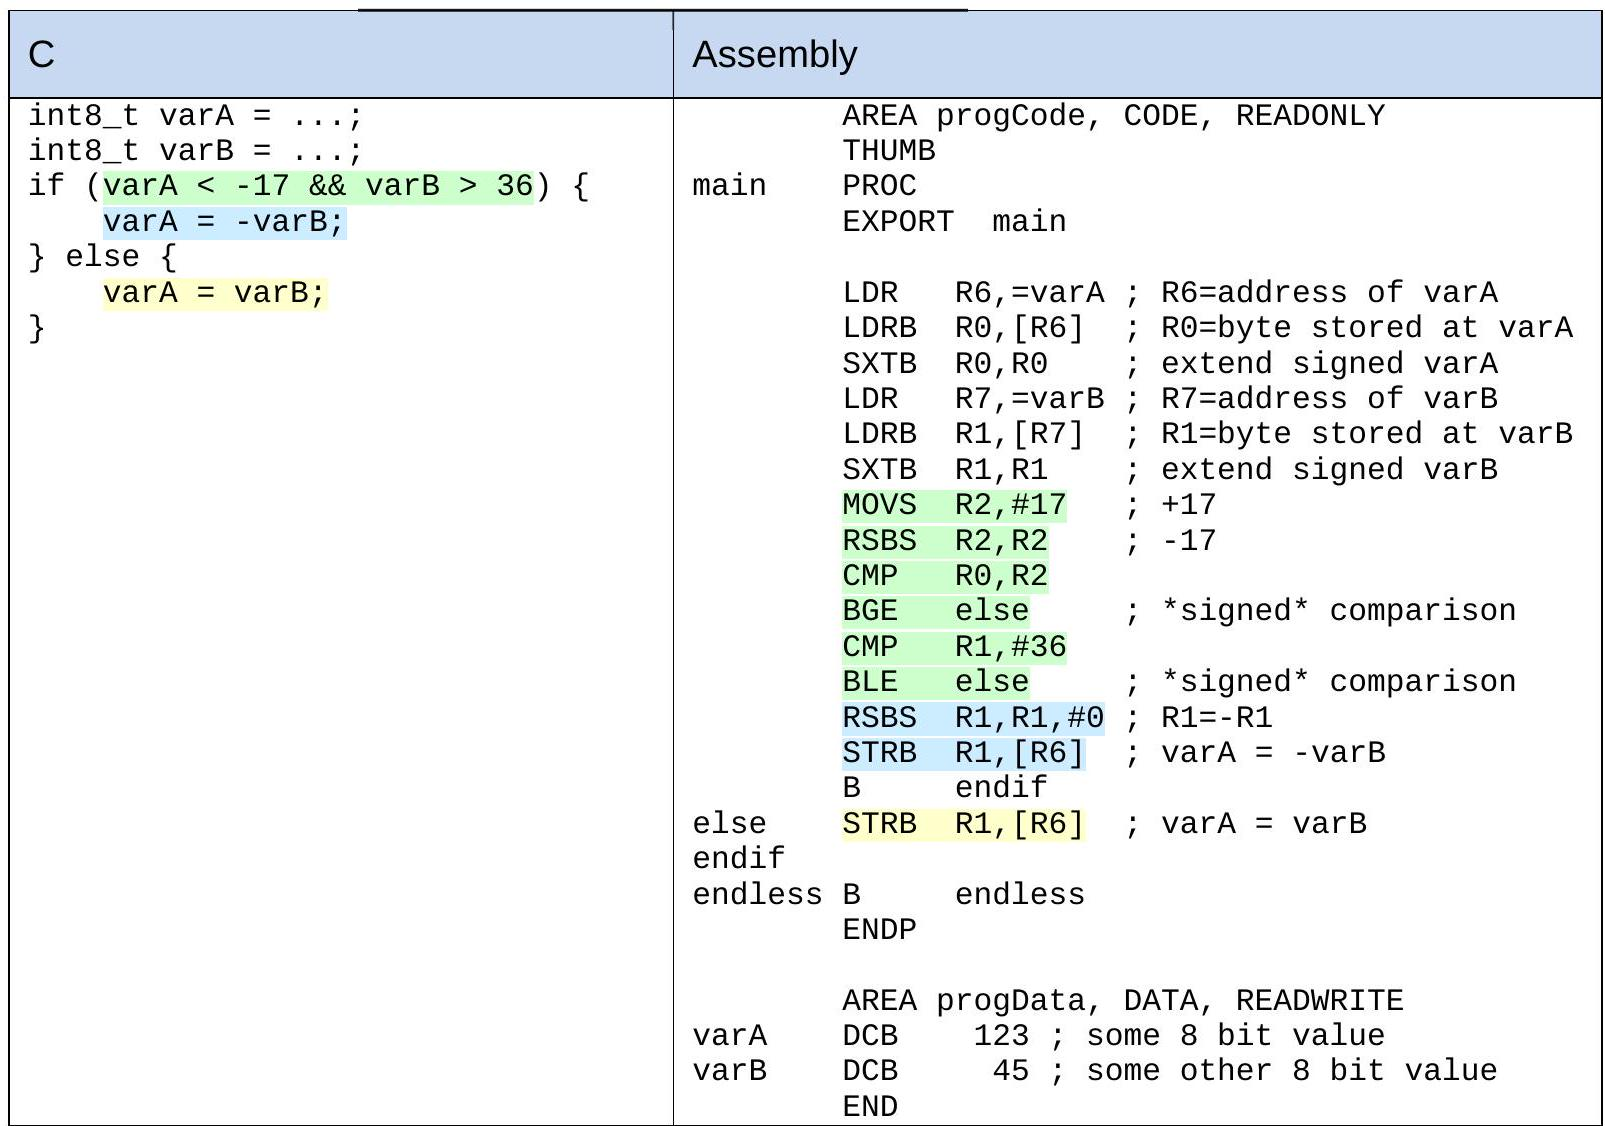
\includegraphics[width=\linewidth]{images/2025_01_02_7eee2d56b23c0199f878g-6(1)}\\
C) If-Then-Else with signed 16-bit variables\\
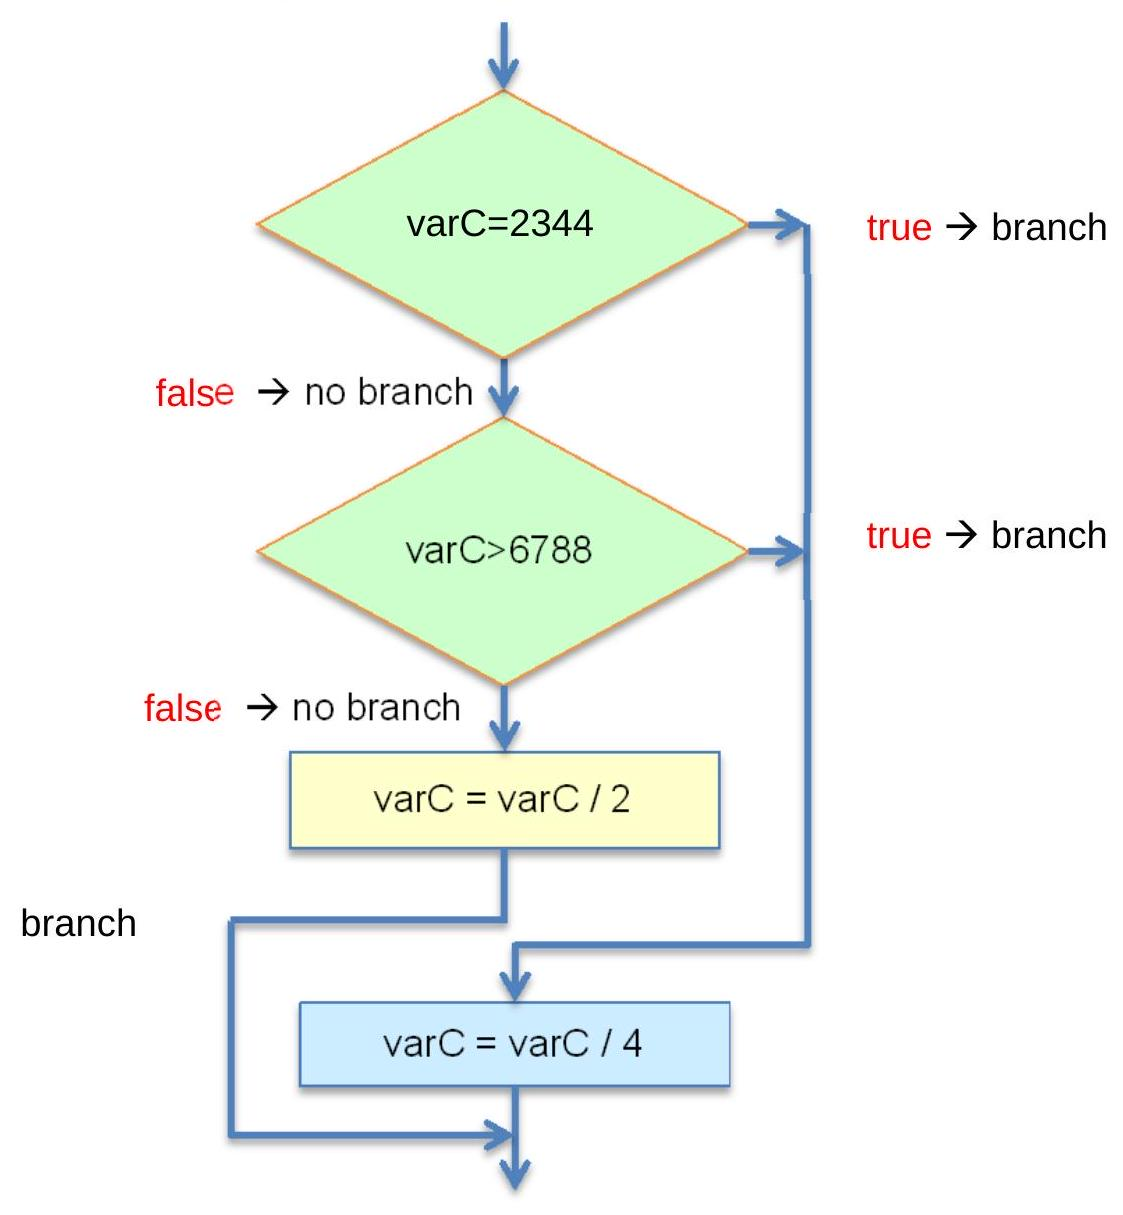
\includegraphics[width=\linewidth]{images/2025_01_02_7eee2d56b23c0199f878g-7(1)}

\begin{center}
\begin{tabular}{|c|c|}
\hline
C & Assembly \\
\hline
\texttt{int16\_t varC = ...; if (varC == 2344 || varC > 6788)\{ varC = varC / 4; \} else \{ varC = varC / 2; \}} & 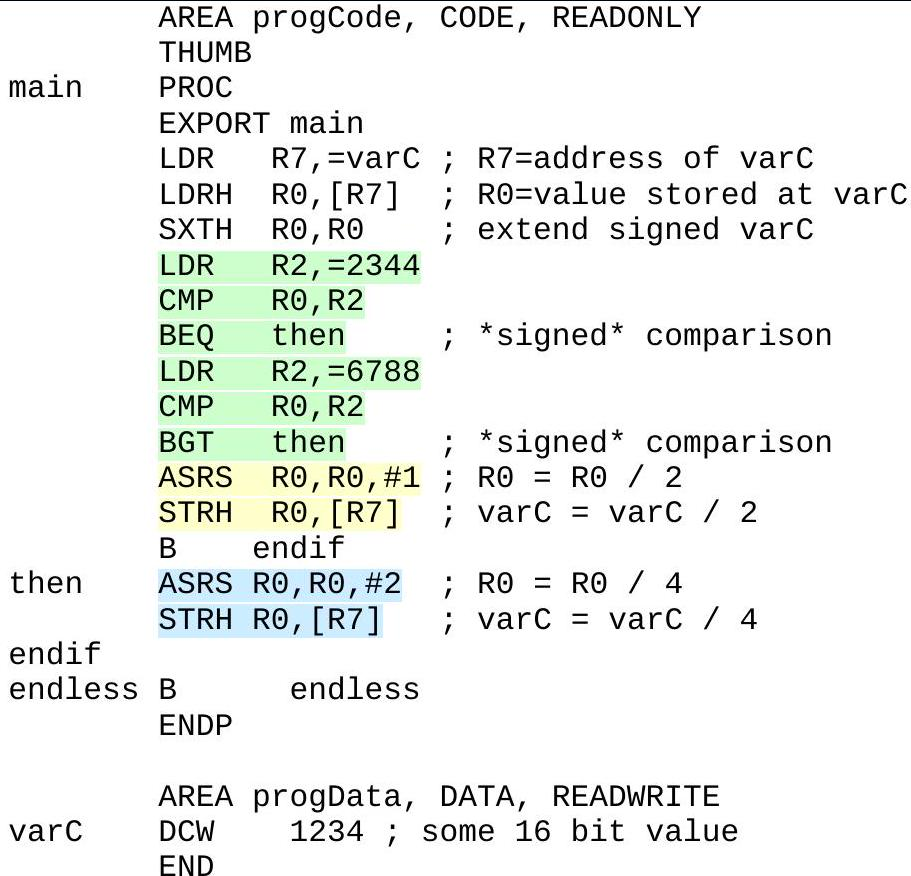
\includegraphics[width=\linewidth]{images/2025_01_02_7eee2d56b23c0199f878g-7}
 \\
\hline
\end{tabular}
\end{center}

\section*{Exercise 2:}
A) For-loop

\begin{center}
\begin{tabular}{|c|c|}
\hline
C & Assembly \\
\hline
\texttt{\#include <utils\_ctboard.h> \#include <stdint.h> ... int32\_t = 0; int32\_t count = 0; for(i = 0; i < 10; i++) \{ count++; \}} & 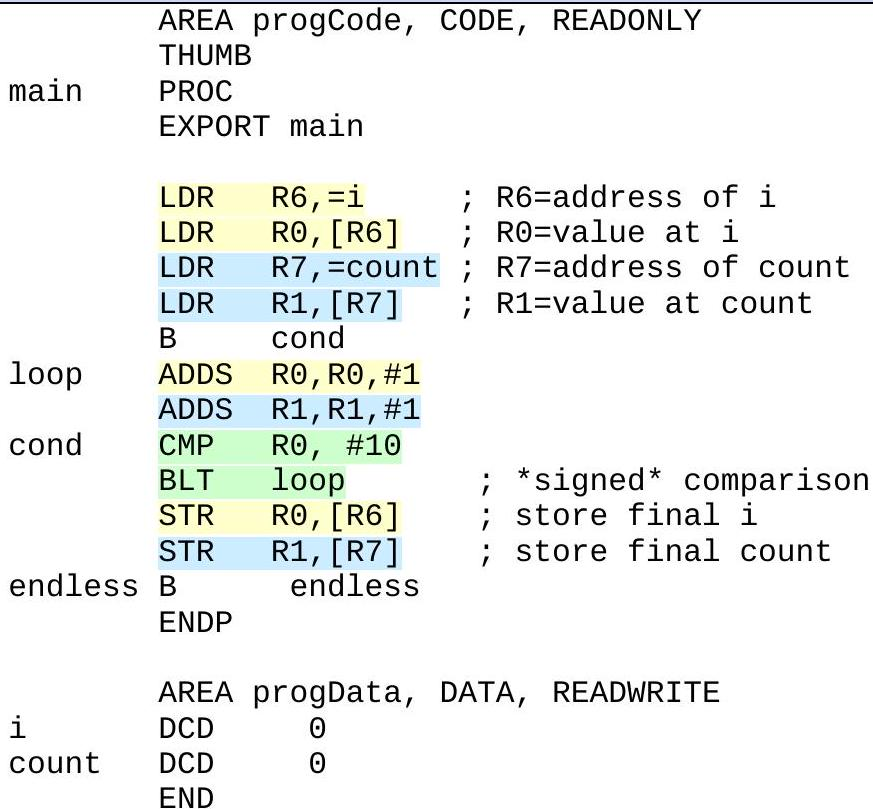
\includegraphics[width=\linewidth]{images/2025_01_02_7eee2d56b23c0199f878g-8}
 \\
\hline
\end{tabular}
\end{center}

B) Compare hand-crafted Assembly version to generated Assembly version\\
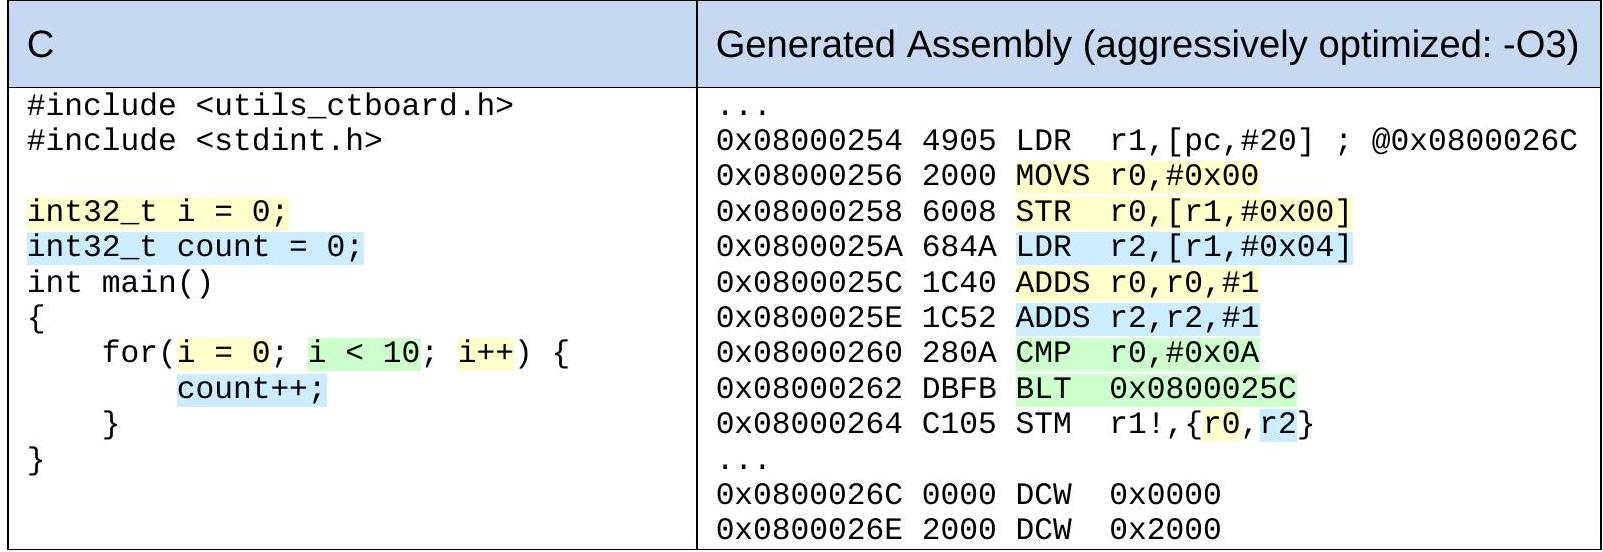
\includegraphics[width=\linewidth]{images/2025_01_02_7eee2d56b23c0199f878g-8(1)}

\section*{Exercise 3:}
A) The structorgram is

\begin{center}
\begin{tabular}{|c|c|}
\hline
\multicolumn{2}{|r|}{$\mathrm{R} 2=0$} \\
\hline
\multicolumn{2}{|l|}{while (R3 = srcstr[R2]) ! $=0$} \\
\hline
\multicolumn{2}{|l|}{\begin{tabular}{l}
\( \text { if (R3 >= } 60 \text { AND R3 <= 90) } \) \\
then else \\
\end{tabular}} \\
\hline
$\mathrm{R} 3=\mathrm{R} 3+32$ &  \\
\hline
\multicolumn{2}{|r|}{outstr[R2] = R3} \\
\hline
\multicolumn{2}{|r|}{INC R2} \\
\hline
\multicolumn{2}{|r|}{outstr[R2] = R3} \\
\hline
\end{tabular}
\end{center}

B) The resulting text is a null terminated string of all caps from the original string: THIS IS MY TESTSTRING
	\raggedcolumns
	\pagebreak
	\section{Control Structures}



\begin{concept}{Control Structure Types}\\
Three fundamental types of control structures:

\textbf{1. Sequence}:
\begin{itemize}
  \item Linear execution of instructions
  \item No branching or decisions
  \item Operations performed in order
\end{itemize}

\textbf{2. Selection}:
\begin{itemize}
  \item Conditional execution (if-then-else)
  \item Branch based on condition
  \item Different paths based on test
\end{itemize}

\textbf{3. Iteration}:
\begin{itemize}
  \item Repeated execution (loops)
  \item Condition-controlled repetition
  \item Fixed number of repetitions
\end{itemize}

Program flow can be represented with three elements:

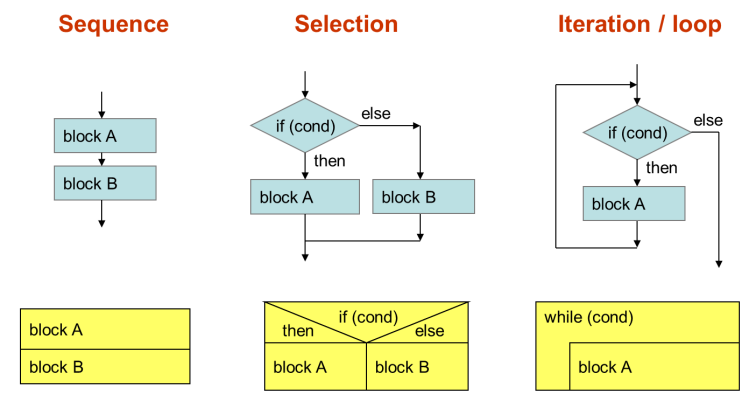
\includegraphics[width=\linewidth]{images/tyoesofcontrolstructures.png}

\begin{itemize}
    \item High level programming language provides these control structures
    \item Compiler translates control structures to assembly using conditional
    and unconditional jumps
\end{itemize}
\end{concept}

\begin{KR}{Implementing Control Structures}\\
Steps for implementing control structures:
\begin{enumerate}
  \item Choose appropriate control structure:
    \begin{itemize}
      \item If-then-else for simple decisions
      \item Switch for multiple cases with same variable
      \item Loops for repeated operations
    \end{itemize}
  \item For switches:
    \begin{itemize}
      \item Create jump table
      \item Calculate offset based on case value
      \item Handle default case
    \end{itemize}
  \item For loops:
    \begin{itemize}
      \item Initialize counter/condition
      \item Place condition check appropriately
      \item Ensure proper exit condition
      \item Update variables correctly
    \end{itemize}
\end{enumerate}
\end{KR}

\begin{remark}
Important considerations:
\begin{itemize}
  \item Consider branch range limitations
  \item Be aware of condition flag changes
  \item Handle corner cases in comparisons
  \item Plan for proper loop termination
  \item Document complex branching logic
\end{itemize}
\end{remark}

\columnbreak


\subsubsection{Selection Structures}


\begin{definition}{IF-ELSE}
    Compiler translates \textbf{selection} into assembly code using conditional and unconditional jumps:\\
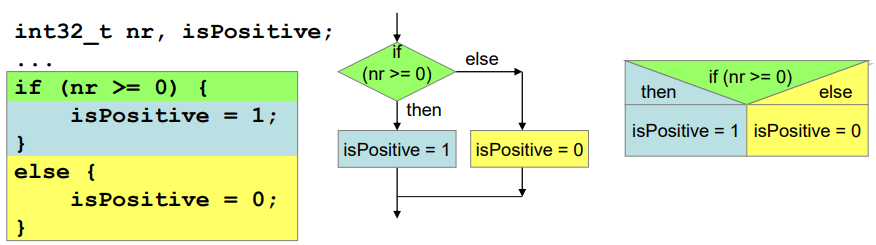
\includegraphics[width=\linewidth]{images/ifelse1.png}

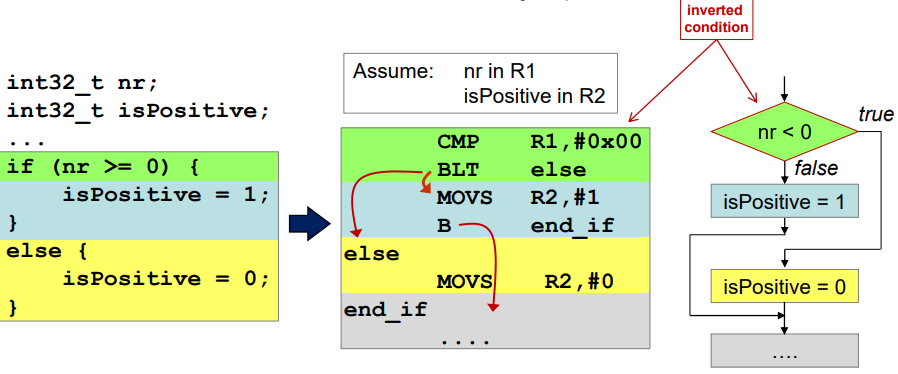
\includegraphics[width=\linewidth]{images/ifelse2.png}
\end{definition}

\begin{KR}{Selection Implementation}

1. Simple if-then:
\begin{lstlisting}[language=armasm, style=basesmol]
    ; if (x > 0) { x++; }
    CMP     R0, #0          ; Compare x with 0
    BLE     endif           ; Skip if x <= 0
    ADDS    R0, #1          ; x++
endif
\end{lstlisting}

2. if-then-else:
\begin{lstlisting}[language=C, style=basesmol]
    if (condition) {    //then-part
    } else {            //else-part
    }
\end{lstlisting}
\vspace{-4mm}
\begin{lstlisting}[language=armasm, style=basesmol]
    CMP     R0, #value      ; Test condition
    BNE     else_part       ; Branch if false
then_part
    ; Then code
    B       endif           ; Skip else
else_part
    ; Else code
endif
    ; Continue execution
\end{lstlisting}

3. Nested if:
\begin{lstlisting}[language=C, style=basesmol]
    if (x > 0) {
        if (y > 0) {
            x = y;
        }
    }
\end{lstlisting}
\vspace{-4mm}
\begin{lstlisting}[language=armasm, style=basesmol]
    CMP     R0, #0          ; Check x > 0
    BLE     endif_outer
    CMP     R1, #0          ; Check y > 0
    BLE     endif_inner
    MOVS    R0, R1          ; x = y
endif_inner
endif_outer
\end{lstlisting}
\end{KR}

\begin{KR}{Selection Implementation} with multiple Conditions

1. Multiple conditions (AND):
\begin{lstlisting}[language=C, style=basesmol]
if (condA && condB) {   //then-part
} else {                //else-part
}
\end{lstlisting}
\vspace{-4mm}
\begin{lstlisting}[language=armasm, style=basesmol]
    ; Test first condition
    CMP     Rx, #valA
    B<cc>   else_label        ; Branch if first fails
    ; Test second condition
    CMP     Ry, #valB
    B<cc>   else_label        ; Branch if second fails

    ; Then part
    <then instructions>
    B       endif_label
    
else_label
    ; Else part
    <else instructions>
    
endif_label
\end{lstlisting}

2. Multiple conditions (OR):
\begin{lstlisting}[language=C, style=basesmol]
if (condA || condB) {   //then-part
} else {                //else-part
}
\end{lstlisting}
\vspace{-4mm}
\begin{lstlisting}[language=armasm, style=basesmol]
    ; Test first condition
    CMP     Rx, #valA
    B<cc>   test_second       ; Try second if first fails
    B       then_label        ; First succeeded
    
test_second
    CMP     Ry, #valB
    B<cc>   else_label        ; Branch if both fail
    
then_label
    ; Then part
    <then instructions>
    B       endif_label
    
else_label
    ; Else part
    <else instructions>
    
endif_label
\end{lstlisting}
\end{KR}

\begin{theorem}{Limitations of Conditional Branches}\\
    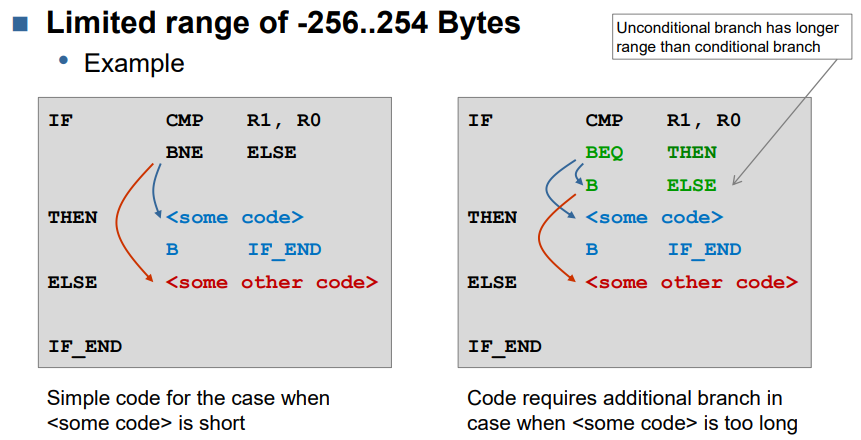
\includegraphics[width=\linewidth]{images/limitsofconditionalbranches.png}
\end{theorem}

\columnbreak

\begin{definition}{Switch-Case}\\
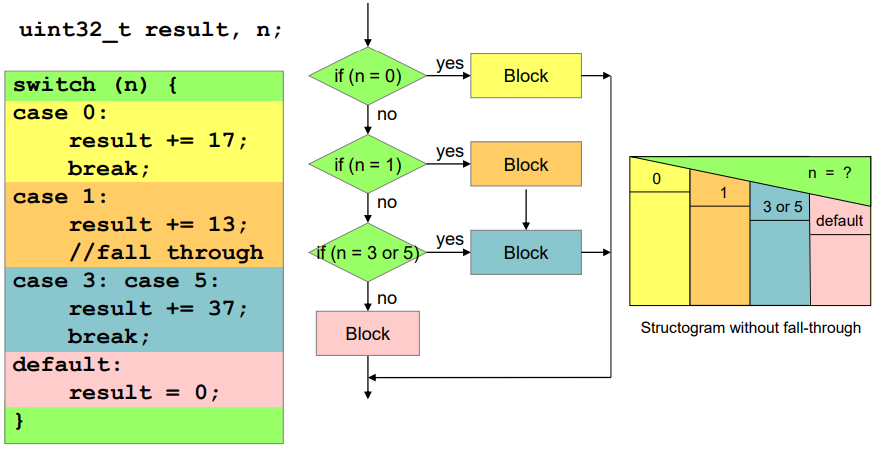
\includegraphics[width=\linewidth]{images/switchcases.png}\\
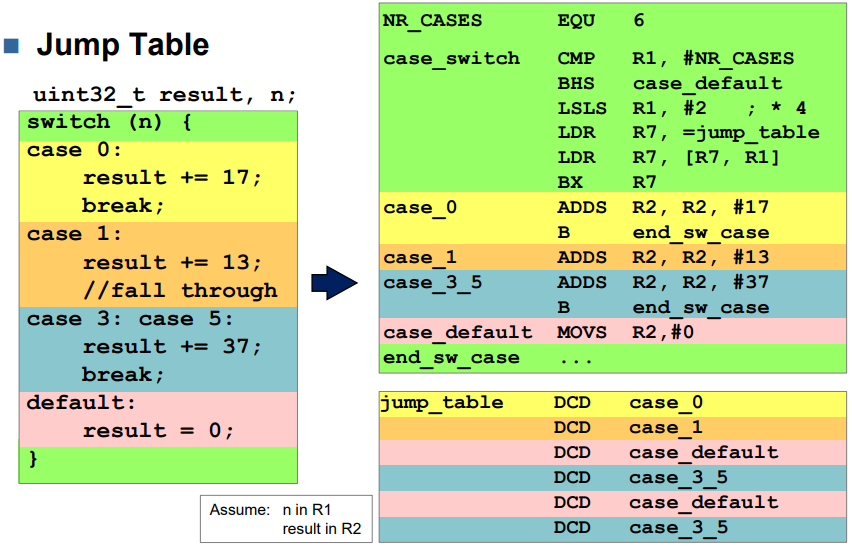
\includegraphics[width=0.9\linewidth]{images/switchcases2.png}
\end{definition}

\begin{KR}{Switch Implementation}

1. Range check and table access:
\begin{lstlisting}[language=armasm, style=basesmol]
    CMP     R0, #MAX_CASES  ; Check range
    BHS     default_case    ; If too high, default
    LSLS    R0, #2          ; Multiply by 4
    LDR     R1, =jump_table ; Load table address
    ADD     R1, R0          ; Add offset
    LDR     R1, [R1]        ; Load target address
    BX      R1              ; Branch to case
\end{lstlisting}

2. Jump table structure:
\begin{lstlisting}[language=armasm, style=basesmol]
jump_table
    DCD     case_0          ; Case 0 handler
    DCD     case_1          ; Case 1 handler
    DCD     default_case    ; Default handler
    ; ... more cases
\end{lstlisting}

3. Case handlers:
\begin{lstlisting}[language=armasm, style=basesmol]
case_0
    ; Handle case 0
    B       switch_end
case_1
    ; Handle case 1
    B       switch_end
default_case
    ; Handle default case
switch_end
\end{lstlisting}
\end{KR}



\begin{example2}{Switch Statement Implementation}
C code example:
\begin{lstlisting}[language=C, style=basesmol]
uint32_t result, n;
switch (n) {
    case 0:
        result += 17;
        break;
    case 1:
        result += 13;
        //fall through
    case 3: 
    case 5:
        result += 37;
        break;
    default:
        result = 0;
}
\end{lstlisting}

Assembly implementation with jump table:
\begin{lstlisting}[language=armasm, style=basesmol]
NR_CASES    EQU     6
case_switch CMP     R1, #NR_CASES
            BHS     case_default
            LSLS    R1, #2        ; * 4
            LDR     R7, =jump_table
            LDR     R7, [R7, R1]
            BX      R7

case_0      ADDS    R2, R2, #17
            B       end_sw_case
case_1      ADDS    R2, R2, #13
case_3_5    ADDS    R2, R2, #37
            B       end_sw_case
case_default MOVS   R2, #0
end_sw_case ...

jump_table  DCD     case_0
            DCD     case_1
            DCD     case_default
            DCD     case_3_5
            DCD     case_default
            DCD     case_3_5
\end{lstlisting}
\end{example2}

\pagebreak

\subsubsection{Loops}

\begin{concept}{Do-While (Post-Test Loop)}:
Compiler translates \textbf{post-test} loops into assembly code using conditional branches:\\
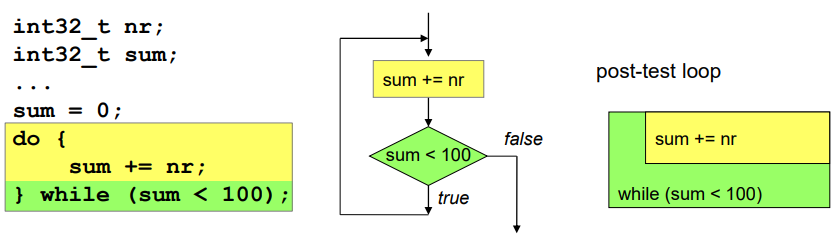
\includegraphics[width=\linewidth]{images/dowhile.png}\\
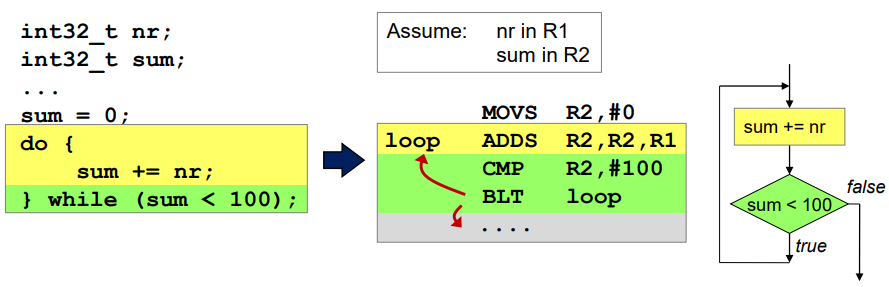
\includegraphics[width=\linewidth]{images/dowhile2.png}
\end{concept}

\begin{KR}{Do-While loop}
\begin{lstlisting}[language=armasm, style=basesmol]
    ; do { x++; } while (x < 10);
do_loop
    ADDS    R0, #1          ; x++
    CMP     R0, #10         ; Check x < 10
    BLT     do_loop         ; Continue if true
\end{lstlisting}
\end{KR}

\begin{concept}{While (Pre-Test Loop)}:
Compiler translates \textbf{pre-test} loops into assembly code reusing structure of do-while:\\
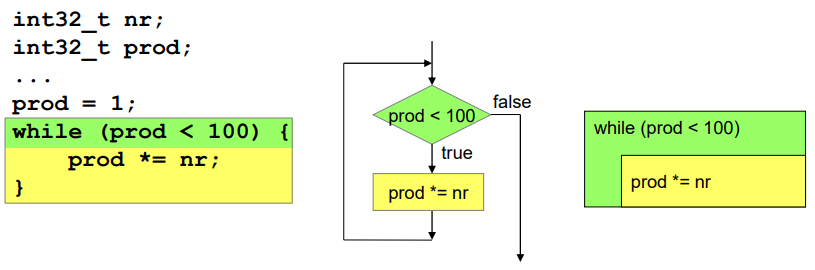
\includegraphics[width=\linewidth]{images/whileloop.png}\\
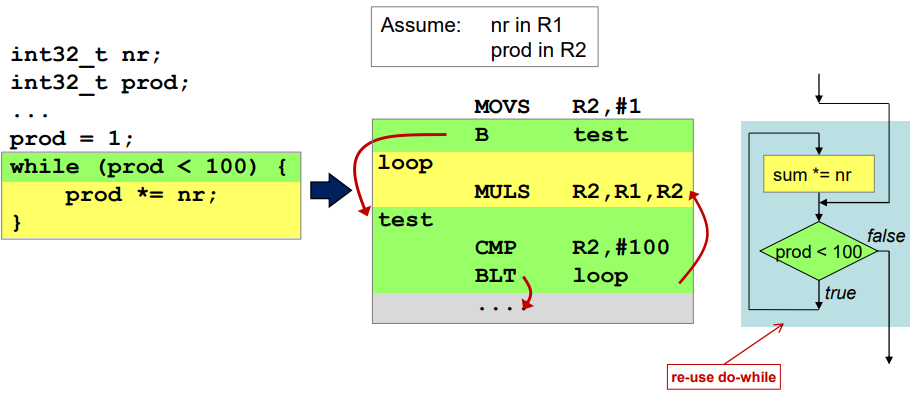
\includegraphics[width=\linewidth]{images/whileloop2.png}
\end{concept}

\begin{KR}{While loop}
\begin{lstlisting}[language=armasm, style=basesmol]
    ; while (x < 10) { x++; }
    B       while_cond      ; Jump to condition
while_loop
    ADDS    R0, #1          ; x++
while_cond
    CMP     R0, #10         ; Check x < 10
    BLT     while_loop      ; Continue if true
\end{lstlisting}
\end{KR}

\begin{concept}{For Loop (Pre-Test Loop)}:\\
For-Loops are converted into while-loops by the compiler.\\
break and continue statements require special treatment.\\
\includegraphics[width=\linewidth]{images/forloop.png}
\end{concept}


\begin{KR}{For loop}
\begin{lstlisting}[language=armasm, style=basesmol]
    ; for (i = 0; i < 10; i++)
    MOVS    R0, #0          ; i = 0
    B       for_cond
for_loop
    ; Loop body
    ADDS    R0, #1          ; i++
for_cond
    CMP     R0, #10         ; Check i < 10
    BLT     for_loop        ; Continue if true
\end{lstlisting}
\end{KR}



\begin{example2}{Complex Control Structure}\\
Implementing nested loops with conditions:

\begin{lstlisting}[language=C, style=basesmol]
for (i = 0; i < 5; i++) {
    if (i == 2) continue;
    for (j = 0; j < 3; j++) {
        if (j == 1) break;
        sum += i + j;
    }
}
\end{lstlisting}
\begin{lstlisting}[language=armasm, style=basesmol]
    MOVS    R0, #0          ; i = 0
outer_loop
    CMP     R0, #2          ; Check i == 2
    BEQ     outer_continue  ; Skip if i == 2
    
    MOVS    R1, #0          ; j = 0
inner_loop
    CMP     R1, #1          ; Check j == 1
    BEQ     outer_continue  ; Break to outer loop
    
    ADDS    R2, R0, R1      ; Calculate i + j
    ADDS    R4, R4, R2      ; Add to sum
    
    ADDS    R1, #1          ; j++
    CMP     R1, #3          ; Check j < 3
    BLT     inner_loop      ; Continue inner loop
    
outer_continue
    ADDS    R0, #1          ; i++
    CMP     R0, #5          ; Check i < 5
    BLT     outer_loop      ; Continue outer loop
\end{lstlisting}
\end{example2}

\subsubsection{String Processing}

\begin{KR}{String Processing Patterns}\\
Common patterns for string manipulation:

1. String traversal:
\begin{lstlisting}[language=armasm, style=basesmol]
    MOVS    R2, #0          ; Index
loop
    LDRB    R3, [R0, R2]    ; Load char
    CMP     R3, #0          ; Check end
    BEQ     done            ; Exit if terminator
    ; Process character
    ADDS    R2, R2, #1      ; Next char
    B       loop
\end{lstlisting}

2. Character transformation:
\begin{lstlisting}[language=armasm, style=basesmol]
    ; Check character range
    CMP     R3, #lower_bound
    BLO     skip            ; Below range
    CMP     R3, #upper_bound
    BHI     skip            ; Above range
    
    ; Transform character
    ADDS    R3, #offset     ; Apply offset
    
skip
    STRB    R3, [R1, R2]    ; Store result
\end{lstlisting}

3. String copy:
\begin{lstlisting}[language=armasm, style=basesmol]
    MOVS    R2, #0          ; Index
copy_loop
    LDRB    R3, [R0, R2]    ; Load source
    STRB    R3, [R1, R2]    ; Store to dest
    ADDS    R2, R2, #1      ; Next char
    CMP     R3, #0          ; Check end
    BNE     copy_loop       ; Continue if not done
\end{lstlisting}
\end{KR}

\begin{remark}
Important considerations:
\begin{itemize}
  \item Choose appropriate conditional branches
  \item Consider signed vs unsigned comparisons
  \item Handle edge cases and termination
  \item Maintain proper register allocation
  \item Document complex control flow
\end{itemize}
\end{remark}

\begin{example2}{String Processing Loop}\\
Converting string to uppercase:
\begin{lstlisting}[language=armasm, style=basesmol]
    AREA    progCode, CODE, READONLY
    THUMB
main
    PROC
    EXPORT  main
    LDR     R0, =srcstr     ; Source string
    LDR     R1, =outstr     ; Output string
    MOVS    R2, #0          ; Initialize index
    
cond
    LDRB    R3, [R0, R2]    ; Load character
    CMP     R3, #0          ; Check for end
    BEQ     endloop         ; Exit if done
    CMP     R3, #60         ; Check if < 'a'
    BLO     store           ; Skip if not lowercase
    CMP     R3, #90         ; Check if > 'z'
    BHI     store           ; Skip if not lowercase
    ADDS    R3, R3, #32     ; Convert to uppercase
    
store
    STRB    R3, [R1, R2]    ; Store character
    ADDS    R2, R2, #1      ; Next character
    B       cond            ; Continue loop
    
endloop
    STRB    R3, [R1, R2]    ; Store terminator
    ENDP
    
srcstr  DCB     "This IS mY TestStriNG", 0
    AREA    progData, DATA, READWRITE
outstr  SPACE   50
\end{lstlisting}

\textbf{Structogram:}\\
\includegraphics[width=0.8\linewidth]{images/structogramstringstuff.png}

\textbf{Result:} "THIS IS MY TESTSTRING"
\end{example2}
	\raggedcolumns
	\subsection{Examples}



\begin{example2}{Selection Structures}
If-Then-Else with unsigned 8-bit variables:

\textbf{Structogram:}\\
\includegraphics[width=0.7\linewidth]{images/structogramex1.png}
\vspace{2mm}\\
\begin{minipage}{0.6\linewidth}
\textbf{Flowchart:}\\
\includegraphics[width=\linewidth]{images/flowchartex1.png}
\end{minipage}
\begin{minipage}{0.38\linewidth}
\textbf{C code:}
\vspace{2mm}\\
\includegraphics[width=\linewidth]{images/ccodeex1.png}
\end{minipage}

\textbf{Assembly code:}\\
\includegraphics[width=\linewidth]{images/assemblycodeex1.png}
\end{example2}

\begin{example2}{Selection Structures}
If-Then-Else with signed 8-bit variables:
\vspace{2mm}\\
\begin{minipage}[t]{0.5\linewidth}
\textbf{Structogram:}\\
\includegraphics[width=\linewidth]{images/structogramex2.png}
\end{minipage}
\begin{minipage}[t]{0.48\linewidth}
\textbf{C code:}
\vspace{2mm}\\
\includegraphics[width=\linewidth]{images/ccodeex2.png}
\end{minipage}

\textbf{Flowchart:}\\
\includegraphics[width=0.7\linewidth]{images/flowchartex2.png}

\textbf{Assembly code:}\\
\includegraphics[width=0.9\linewidth]{images/assemblycodeex2.png}
\end{example2}

\begin{example2}{Selection Structures}
If-Then-Else with signed 16-bit variables:
\vspace{2mm}\\
\begin{minipage}[t]{0.5\linewidth}
\textbf{Structogram:}\\
\includegraphics[width=\linewidth]{images/structogramex3.png}
\end{minipage}
\begin{minipage}[t]{0.48\linewidth}
\textbf{C code:}
\vspace{2mm}\\
\includegraphics[width=\linewidth]{images/ccodeex3.png}
\end{minipage}

\textbf{Flowchart:}\\
\includegraphics[width=0.7\linewidth]{images/flowchartex3.png}

\textbf{Assembly code:}\\
\includegraphics[width=\linewidth]{images/assemblycodeex3.png}
\end{example2}



\begin{example2}{For-Loop Implementation}\\
Example for-loop in C and assembly:

\begin{lstlisting}[language=C, style=basesmol]
// C code with volatile variables
volatile int32_t i = 0;
volatile int32_t count = 0;
for(i = 0; i < 10; i++) {
    count++;
}
\end{lstlisting}

Assembly implementation:
\begin{lstlisting}[language=armasm, style=basesmol]
    AREA    progCode, CODE, READONLY
    THUMB
main
    PROC
    EXPORT  main
    
    LDR     R6, =i          ; R6 = address of i
    LDR     R0, [R6]        ; R0 = value at i
    LDR     R7, =count      ; R7 = address of count
    LDR     R1, [R7]        ; R1 = value at count
    B       cond
    
loop
    ADDS    R0, R0, #1      ; Increment i
    ADDS    R1, R1, #1      ; Increment count
cond
    CMP     R0, #10
    BLT     loop            ; Branch if i < 10
    
    STR     R0, [R6]        ; Store final i
    STR     R1, [R7]        ; Store final count
    ENDP
\end{lstlisting}

Compiler-optimized version:
\begin{lstlisting}[language=armasm, style=basesmol]
    LDR     r1, [pc, #20]   ; Load address
    MOVS    r0, #0          ; Initialize counter
    STR     r0, [r1, #0]    ; Store i
    LDR     r2, [r1, #4]    ; Load count
    
increment
    ADDS    r0, r0, #1      ; i++
    ADDS    r2, r2, #1      ; count++
    CMP     r0, #10         ; Check condition
    BLT     increment       ; Loop if i < 10
    STM     r1!, {r0, r2}   ; Store final values
\end{lstlisting}
\end{example2}


	\pagebreak
	\section{Subroutines and Stack}

\subsubsection{Subroutine}

\begin{concept}{Subroutines}
Key elements of subroutines:
\begin{itemize}
  \item Label to identify subroutine entry point
  \item Return instruction (BX LR) to exit
  \item Proper register management
\end{itemize}
\end{concept}





\begin{concept}{Call and Return Mechanism}
Basic subroutine mechanics:
\begin{itemize}
  \item \textbf{BL (Branch with Link)}:
    \begin{itemize}
      \item Stores current PC in LR (R14)
      \item Branches to subroutine address
      \item Direct and relative addressing
    \end{itemize}
  \item \textbf{BLX (Branch with Link and Exchange)}:
    \begin{itemize}
      \item Similar to BL but with register-specified target
      \item Indirect and absolute addressing
    \end{itemize}
  \item \textbf{Return}: Using BX LR or POP {..., PC} if LR was saved
\end{itemize}
\end{concept}

\begin{theorem}{Subroutine Calling Convention and Register Usage}
\begin{itemize}
  \item \textbf{Calling Convention}:
    \begin{itemize}
      \item Parameters passed in R0-R3
      \item Return value in R0
      \item Link Register (LR) for return address
      \item Stack for additional parameters/locals
    \end{itemize}
  \item \textbf{Register Usage}:
    \begin{itemize}
      \item R0-R3: Parameters and scratch
      \item R4-R11: Must be preserved
      \item R12: IP (scratch)
      \item R13: SP (stack pointer)
      \item R14: LR (link register)
      \item R15: PC (program counter)
    \end{itemize}
\end{itemize}
\end{theorem}

\begin{example2}{Subroutine Call and Return}
Multiply by 3 implementation:
\begin{lstlisting}[language=armasm, style=basesmol]
MulBy3  MOV     R4, R0      ; Save input value
        LSLS    R0, #1      ; Multiply by 2
        ADD     R0, R4      ; Add original value
        BX      LR          ; Return
\end{lstlisting}

\begin{minipage}{0.58\linewidth}
\includegraphics[width=\linewidth]{images/subroutine.png}
\end{minipage}
\begin{minipage}{0.4\linewidth}
in detail:
\begin{itemize}
  \item Label with name \textcolor{darkred}{\textbf{MulBy3}}
  \item Return Statement \textcolor{darkblue}{\textbf{BX LR}}
\end{itemize}
\end{minipage}
\end{example2}

\begin{KR}{Using Subroutines and Stack}
Steps for implementing subroutines:
\begin{enumerate}
  \item Define subroutine entry point with label
  \item Save registers that will be modified
    \begin{itemize}
      \item Use PUSH at start
      \item Include LR if calling other subroutines
    \end{itemize}
  \item Implement subroutine logic
  \item Restore registers in reverse order
    \begin{itemize}
      \item Use POP before return
      \item Can return using POP {..., PC} if LR was saved
    \end{itemize}
  \item Return using BX LR if LR wasn't saved
\end{enumerate}
\end{KR}

\begin{remark}
Important considerations:
\begin{itemize}
  \item Always maintain stack alignment
  \item Match PUSH/POP pairs exactly
  \item Be careful with SP manipulation
  \item Consider nesting depth for stack space
\end{itemize}
\end{remark}

\begin{KR}{Subroutine Implementation}\\
Guidelines for implementing subroutines:

1. Basic subroutine:
\begin{lstlisting}[language=armasm, style=basesmol]
proc_name
    PUSH    {LR}           ; Save return address
    ; Subroutine code
    POP     {PC}           ; Return
\end{lstlisting}

2. With register preservation:
\begin{lstlisting}[language=armasm, style=basesmol]
proc_name
    PUSH    {R4-R7, LR}    ; Save modified registers
    ; Subroutine code using R4-R7
    POP     {R4-R7, PC}    ; Restore and return
\end{lstlisting}

3. With local variables:
\begin{lstlisting}[language=armasm, style=basesmol]
proc_name
    PUSH    {R4, LR}       ; Save registers
    SUB     SP, SP, #8     ; Allocate locals
    ; Use [SP] to [SP, #4] for locals
    ADD     SP, SP, #8     ; Deallocate locals
    POP     {R4, PC}       ; Restore and return
\end{lstlisting}
\end{KR}

\begin{example2}{Nested Subroutine Calls}\\
Example of multiple nested calls with stack manipulation:
\begin{lstlisting}[language=armasm, style=basesmol]
    AREA    progCode, CODE, READONLY
    THUMB
main
    LDR     R1, =0x10203040     ; Initial values
    LDR     R2, =0x50607080
    BL      procA               ; Call procA
    BL      procB               ; Call procB
    B       endless

procA
    PUSH    {R1, R2}            ; Save registers
    LDR     R1, =0xAABBCCDD     ; New values
    LDR     R2, =0xEEFF1020
    POP     {R1, R2}            ; Restore registers
    BX      LR                  ; Return

procB
    PUSH    {R1, R2, LR}        ; Save including LR
    LDR     R1, =0x11223344     ; New values
    LDR     R2, =0x55667788
    BL      procC               ; Call procC
    POP     {R1, R2, PC}        ; Return by popping PC

procC
    PUSH    {R1, R2, LR}        ; Save registers
    LDR     R1, =0x11111111     ; New values
    LDR     R2, =0x22222222
    BL      procD               ; Call procD
    POP     {R1, R2, PC}        ; Return by popping PC
\end{lstlisting}

Stack contents at key points:
\begin{itemize}
  \item After procA PUSH: R1(0x10203040), R2(0x50607080)
  \item After procB PUSH: R1, R2, LR(ret\_addr)
  \item After procC PUSH: R1(0x11223344), R2(0x55667788), LR(ret\_addr)
\end{itemize}
\end{example2}



\subsubsection{Stack}

\begin{definition}{Stack}characteristics:
\begin{itemize}
  \item \textcolor{darkblue}{\textbf{Stack Area}} (Section): Continuous RAM section
  \item \textcolor{darkred}{\textbf{Stack Pointer (SP)}}: R13, points to last written value
  \item \textbf{Direction}: Full-descending (grows toward lower addresses)
  \item \textbf{Alignment}: Word-aligned (4 bytes)
  \item \textbf{Data Size}: 32-bit words only
\end{itemize}

Main operations:
\begin{itemize}
  \item \textcolor{darkgreen}{\textbf{PUSH}}: Decrements SP, then stores words
  \item \textcolor{darkgreen}{\textbf{POP}}: Loads words, then increments SP
\end{itemize}

Stack constraints:
\begin{itemize}
  \item Number of PUSH and POP operations must match
  \item SP must stay between stack-limit and stack-base\\
  $\rightarrow$ \textcolor{darkgreen}{Stack-limit} $\leq$ SP $\leq$ \textcolor{darkpurple}{Stack-base}
\end{itemize}

\includegraphics[width=\linewidth]{images/stack_overview.png}


\end{definition}

\begin{concept}{Stack Instructions}
Special stack manipulation instructions:
\vspace{1mm}\\
\begin{minipage}[t]{0.5\linewidth}
\begin{itemize}
  \item \textbf{ADD/SUB SP}:
    \begin{itemize}
      \item Immediate offset 0-508
      \item Must be multiple of 4
    \end{itemize}
  \item \textbf{SP-relative LDR/STR}:
    \begin{itemize}
      \item Immediate offset 0-1020
      \item Used for frame access
    \end{itemize}
\end{itemize}
\end{minipage}
\begin{minipage}[t]{0.5\linewidth}
\begin{itemize}
  \item \textbf{PUSH/POP}:
    \begin{itemize}
      \item Multiple register transfer
      \item Maintains alignment
      \item Can include PC/LR
    \end{itemize}
\end{itemize}
\end{minipage}
\end{concept}



\begin{example2}{PUSH/POP Implementation}

  \includegraphics[width=\linewidth]{images/2024_12_29_79e6b22f503fb7b4f718g-08}
\begin{lstlisting}[language=armasm, style=basesmol]
; PUSH {R2,R3,R6}
SUB     SP, SP, #12     ; Reserve stack space
STR     R2, [SP]        ; Store R2
STR     R3, [SP, #4]    ; Store R3
STR     R6, [SP, #8]    ; Store R6

; POP {R2,R3,R6}
LDR     R2, [SP]        ; Restore R2
LDR     R3, [SP, #4]    ; Restore R3
LDR     R6, [SP, #8]    ; Restore R6
ADD     SP, SP, #12     ; Free stack space
\end{lstlisting}
\end{example2}

\subsubsection{Stack Operations and Functions}

\begin{concept}{Stack Operations}
Common stack manipulation patterns:
\begin{itemize}
  \item \textbf{Register Save/Restore}:
    \begin{itemize}
      \item PUSH/POP for callee-saved registers
      \item Multiple register transfer
    \end{itemize}
  \item \textbf{Local Variables}:
    \begin{itemize}
      \item SUB SP to allocate space
      \item Access via SP-relative addressing
      \item ADD SP to deallocate space
    \end{itemize}
  \item \textbf{Return Handling}:
    \begin{itemize}
      \item Save LR if making calls
      \item Return via BX LR or POP \{PC\}
      \item Use PC in POP list when LR saved
    \end{itemize}
\end{itemize}
\end{concept}

\begin{KR}{Function Implementation Patterns}

1. Simple function:
\begin{lstlisting}[language=armasm, style=basesmol]
func    PUSH    {LR}        ; Save return address
        ; Function body
        POP     {PC}        ; Return
\end{lstlisting}

2. Function with locals:
\begin{lstlisting}[language=armasm, style=basesmol]
func    PUSH    {R4, LR}    ; Save registers
        SUB     SP, #8      ; Space for locals
        ; Function body
        ADD     SP, #8      ; Remove locals
        POP     {R4, PC}    ; Return
\end{lstlisting}

3. Function with parameters:
\begin{lstlisting}[language=armasm, style=basesmol]
        ; R0-R3 = first 4 parameters
        ; [SP] = fifth parameter
func    PUSH    {R4-R6, LR} ; Save registers
        LDR     R4, [SP, #16] ; Load 5th param
        ; Function body
        POP     {R4-R6, PC} ; Return
\end{lstlisting}
\end{KR}

\begin{example2}{Stack Frame}
Example of complete function:
\begin{lstlisting}[language=armasm, style=basesmol]
; int calc(int a, int b, int c)
; a in R0, b in R1, c in R2
calc    PUSH    {R4-R6, LR} ; Save registers
        ; Save parameters
        MOVS    R4, R0      ; Save a
        MOVS    R5, R1      ; Save b
        MOVS    R6, R2      ; Save c
        ; Call helper function
        MOVS    R0, R4      ; First param
        BL      helper      ; Call helper
        ; Continue calculation
        ADDS    R0, R5      ; Add b
        ADDS    R0, R6      ; Add c
        
        POP     {R4-R6, PC} ; Return
\end{lstlisting}
\end{example2}

\begin{remark}
Stack usage considerations:
\begin{itemize}
  \item Monitor stack depth in nested calls
  \item Always maintain 8-byte alignment for SP
  \item Consider register usage to minimize stack operations
  \item Be aware of stack space in interrupt handlers
  \item Document stack requirements for functions
\end{itemize}
\end{remark}

\columnbreak

\subsubsection{Stack Frame}

\begin{definition}{Stack Frame Structure}
Components of a stack frame:
\begin{itemize}
  \item \textbf{Saved Registers}:
    \begin{itemize}
      \item Caller-saved (R0-R3, R12)
      \item Callee-saved (R4-R11)
      \item Link register (LR)
    \end{itemize}
  \item \textbf{Local Variables}:
    \begin{itemize}
      \item Allocated on stack if needed
      \item Word-aligned access
    \end{itemize}
  \item \textbf{Parameters}:
    \begin{itemize}
      \item Beyond R0-R3 if needed
      \item Pushed by caller
    \end{itemize}
\end{itemize}

\end{definition}


\begin{KR}{Stack Frame Layout/Management}\\
Steps for function prologue and epilogue, and guidelines for managing stack frames:

1. Frame structure:
\begin{itemize}
  \item Previous stack frame
  \item Return address (LR)
  \item Saved registers
  \item Local variables
  \item Parameters for called functions
\end{itemize}

2. Frame creation/Function prologue:
\begin{lstlisting}[language=armasm, style=basesmol]
    ; Save registers and create frame
    PUSH    {R4-R7, LR}    ; Save registers
    SUB     SP, SP, #frame_size  ; Allocate space
    SUB     SP, SP, #locals ; Allocate local vars
    
    ; Initialize frame if needed
    MOV     R4, #0         ; Clear locals
    STR     R4, [SP, #0]   ; Initialize var1
    STR     R4, [SP, #4]   ; Initialize var2
\end{lstlisting}

3. Stack frame access:
\begin{lstlisting}[language=armasm, style=basesmol]
    ; Access local variables
    LDR     R0, [SP, #offset1]  ; Load local1
    STR     R1, [SP, #offset2]  ; Store to local2

    ; Access parameters
    LDR     R0, [SP, #20]   ; First stack parameter
    ; Access parameters beyond R0-R3
    LDR     R0, [SP, #param_offset] ; Load param
\end{lstlisting}

4. Frame cleanup/Function epilogue:
\begin{lstlisting}[language=armasm, style=basesmol]
    ; Deallocate frame and restore
    ADD     SP, SP, #frame_size  ; Remove locals
    ADD     SP, SP, #locals ; Deallocate locals
    POP     {R4-R7, PC}    ; Restore and return
\end{lstlisting}
\end{KR}

\begin{remark}
Important considerations:
\begin{itemize}
  \item Maintain 8-byte stack alignment
  \item Save LR before any BL instructions
  \item Properly pair PUSH/POP operations
  \item Document stack frame layout
  \item Track stack depth in nested calls
\end{itemize}
\end{remark}



\begin{example2}{Stack Frame Management} Stack frame creation and cleanup:
\begin{lstlisting}[language=armasm, style=basesmol]
func    ; Function prologue
    PUSH    {R4-R8, LR}    ; Save registers
    SUB     SP, SP, #12    ; Allocate locals
    ; Access local variables relative to SP
    STR     R0, [SP, #0]   ; Local var 1
    STR     R1, [SP, #4]   ; Local var 2
    STR     R2, [SP, #8]   ; Local var 3
    ; Function body
    BL      other_func     ; Call another function
    ; Function epilogue
    ADD     SP, SP, #12    ; Deallocate locals
    POP     {R4-R8, PC}    ; Restore and return
\end{lstlisting}
\end{example2}



















	\raggedcolumns
	\subsection{Examples}







\begin{KR}{Stack Initialization and Memory Layout}

1. Stack Organization:
\begin{lstlisting}[language=armasm, style=basesmol]
; Memory Layout
0x20030000  Stack-base (initial SP value)
           | Stack grows downward
0x20020000  |
           | Available stack space
0x20010000  |
0x20000000  Start of SRAM (Stack-limit)
\end{lstlisting}

2. Initialization Process:
\begin{itemize}
  \item At reset, processor loads initial SP from address 0x00000000
  \item Vector table first entry contains Stack-base address
  \item SP initialized to this value before any code execution
\end{itemize}

3. Setting Stack Base Address:
\begin{lstlisting}[language=armasm, style=basesmol]
    AREA    RESET, DATA, READONLY
    EXPORT  __Vectors
__Vectors
    DCD     0x20030000      ; Initial SP value
    DCD     Reset_Handler   ; Reset vector
    ; Rest of vector table...
\end{lstlisting}

4. Determining Stack Size:
\begin{itemize}
  \item Calculate maximum stack depth:
    \begin{itemize}
      \item Count local variables
      \item Consider nested function calls
      \item Include interrupt handler needs
    \end{itemize}
  \item Add safety margin (e.g., 20\%)
  \item Ensure stack stays within SRAM bounds
\end{itemize}

5. Stack Pointer Rules:
\begin{itemize}
  \item Must be word-aligned (multiple of 4)
  \item Must point to valid SRAM
  \item Must not overlap with other memory regions
  \item Stack-limit < SP <= Stack-base always true
\end{itemize}

6. Example Stack Size Calculation:
\begin{lstlisting}[language=armasm, style=basesmol]
; Example for a simple program
Local vars:        20 bytes
Function params:   16 bytes
Saved registers:   32 bytes
Nested calls:      24 bytes
ISR overhead:      32 bytes
Safety margin:     25 bytes (20%)
------------------------
Total needed:     149 bytes

; Round up to nearest word boundary
Actual allocation: 152 bytes (38 words)
\end{lstlisting}
\end{KR}



\begin{KR}{Stack Analysis in Nested Subroutine Calls} from exercise sheet 8\\
Steps to analyze stack content in nested subroutine calls:

\textbf{1. Track initial stack pointer value}: Note starting SP value
\begin{itemize}
  \item Stack grows downward in memory
\end{itemize}

\textbf{2. For each PUSH instruction}: Subtract 4 bytes per register
\begin{itemize}
  \item Write values in order specified
  \item Remember which subroutine saved what
\end{itemize}

\textbf{3. For subroutine calls (BL)}: LR gets set to return address
\begin{itemize}
  \item If LR needs to be saved (nested calls), it must be PUSHed
\end{itemize}

\textbf{4. Keep track through nested calls}:
\begin{itemize}
  \item Each nested level maintains its own stack frame
  \item Stack unwinds in reverse order when returning
\end{itemize}
\end{KR}

\begin{example2}{Simple Stack Analysis}\\
Consider this simple nested call sequence:

\begin{lstlisting}[language=armasm, style=basesmol]
main    ; SP = 0x20002000
        LDR     R0, =0x11111111
        LDR     R1, =0x22222222
        BL      funcA          ; Z1
        B       endless

funcA   PUSH    {R0, R1, LR}  ; Z2
        BL      funcB
        POP     {R0, R1, PC}

funcB   PUSH    {R4, LR}      ; Z3
        MOVS    R4, #42
        POP     {R4, PC}
\end{lstlisting}

Stack contents at Z1, Z2, Z3:

\begin{lstlisting}[style=basesmol]
Z1: Stack is empty, SP = 0x20002000

Z2: Stack from top (higher address):           
0x20001FF4: Return addr to main
0x20001FF0: 0x22222222 (R1)
0x20001FEC: 0x11111111 (R0)
SP = 0x20001FEC

Z3: Stack from top (higher address):
0x20001FE4: Return addr to funcA
0x20001FE0: R4 value
0x20001FF4: Return addr to main (from Z2)
0x20001FF0: 0x22222222 (R1 from Z2)
0x20001FEC: 0x11111111 (R0 from Z2)
SP = 0x20001FE0
\end{lstlisting}
\end{example2}

\begin{KR}{Stack Frame Management Patterns}
Guidelines for managing stack frames:

1. Basic frame setup:
\begin{lstlisting}[language=armasm, style=basesmol]
function_start
    ; Save registers and create frame
    PUSH    {R4-R7, LR}     ; Save modified registers
    SUB     SP, SP, #12     ; Allocate local variables
    
    ; Function body...
    
    ; Clean up frame and return
    ADD     SP, SP, #12     ; Deallocate locals
    POP     {R4-R7, PC}     ; Restore and return
\end{lstlisting}

2. Accessing stack variables:
\begin{lstlisting}[language=armasm, style=basesmol]
    ; Local variable access
    STR     R0, [SP, #0]    ; First local variable
    STR     R1, [SP, #4]    ; Second local variable
    
    ; Later access
    LDR     R0, [SP, #0]    ; Load first variable
    LDR     R1, [SP, #4]    ; Load second variable
\end{lstlisting}

3. Nested function calls:
\begin{lstlisting}[language=armasm, style=basesmol]
outer_func
    PUSH    {R4-R6, LR}     ; Save registers
    ; Function body...
    BL      inner_func      ; Call inner function
    ; Continue processing...
    POP     {R4-R6, PC}     ; Return
\end{lstlisting}
\end{KR}

\begin{example2}{Stack-Based Local Variables}
Example of managing local array on stack:
\begin{lstlisting}[language=armasm, style=basesmol]
process_data
    PUSH    {R4-R7, LR}     ; Save registers
    SUB     SP, SP, #16     ; Space for 4-word array
    
    ; Initialize array on stack
    MOVS    R0, #1          
    STR     R0, [SP, #0]    ; array[0] = 1
    MOVS    R0, #2
    STR     R0, [SP, #4]    ; array[1] = 2
    
    ; Process array elements
    LDR     R1, [SP, #0]    ; Load array[0]
    LDR     R2, [SP, #4]    ; Load array[1]
    ADDS    R0, R1, R2      ; Compute sum
    
    ; Clean up and return
    ADD     SP, SP, #16     ; Remove local array
    POP     {R4-R7, PC}     ; Return
\end{lstlisting}

Key points:
\begin{itemize}
  \item Allocate space with SUB SP
  \item Access relative to SP
  \item Clean up stack before return
\end{itemize}
\end{example2}

\begin{KR}{Reentrant Function Implementation}
Guidelines for writing reentrant functions:

1. Save all modified registers:
\begin{lstlisting}[language=armasm, style=basesmol]
    ; R0-R3 are caller-saved
    PUSH    {R4-R7, LR}     ; Save callee-saved
    
    ; Use R4-R7 for local variables
    MOV     R4, R0          ; Save parameter
    
    ; Restore before return
    POP     {R4-R7, PC}
\end{lstlisting}

2. Use stack for local storage:
\begin{lstlisting}[language=armasm, style=basesmol]
    ; Allocate local storage
    SUB     SP, SP, #8      ; Two local variables
    STR     R0, [SP, #0]    ; Save first value
    STR     R1, [SP, #4]    ; Save second value
    
    ; Access locals via SP
    LDR     R0, [SP, #0]    ; Load first value
\end{lstlisting}

3. Handle nested calls:
\begin{lstlisting}[language=armasm, style=basesmol]
    ; Save state before nested call
    PUSH    {R4, LR}        ; Save working register
    BL      other_func      ; Make nested call
    POP     {R4, PC}        ; Restore and return
\end{lstlisting}
\end{KR}

\begin{example2}{Recursive Function}
Implementation of recursive factorial calculation:
\begin{lstlisting}[language=armasm, style=basesmol]
factorial
    ; Input in R0, result in R0
    PUSH    {R4, LR}        ; Save registers
    MOVS    R4, R0          ; Save n
    
    CMP     R0, #1          ; Check base case
    BLE     fact_end        ; Return 1 if n <= 1
    
    SUBS    R0, R0, #1      ; n-1
    BL      factorial       ; Recursive call
    MULS    R0, R4, R0      ; n * factorial(n-1)
    B       fact_return
    
fact_end
    MOVS    R0, #1          ; Return 1
    
fact_return
    POP     {R4, PC}        ; Return
\end{lstlisting}

Stack growth pattern:
\begin{itemize}
  \item Each call adds 8 bytes (R4, LR)
  \item Maximum depth = n-1 calls
  \item Stack unwinds on returns
\end{itemize}
\end{example2}


	\raggedcolumns
	\pagebreak
	\section{Parameter Passing}

\begin{concept}{Parameter Passing Methods}\\
Data can be passed between functions through:
\begin{itemize}
  \item \textbf{Registers}: Fast, limited number available
  \item \textbf{Global Variables}: Shared memory space
  \item \textbf{Stack}: 
    \begin{itemize}
      \item Caller: PUSH parameters onto stack
      \item Callee: Access via LDR from stack
    \end{itemize}
\end{itemize}
\end{concept}

\begin{definition}{ARM Procedure Call Standard}\\
\textbf{Parameter Passing:}
\begin{itemize}
  \item First four arguments use R0-R3
  \item Additional parameters go on stack
\end{itemize}

\textbf{Return Values:}
\begin{itemize}
  \item \textbf{Small Values} ($\leqslant$ 32 bits): 
    \begin{itemize}
      \item Return in R0
      \item Zero/sign extend if needed
    \end{itemize}
  \item \textbf{Double Word} (64 bits): R0/R1
  \item \textbf{128-bit Values}: R0-R3
  \item \textbf{Larger Values}: 
    \begin{itemize}
      \item Store in memory
      \item Return pointer in R0
    \end{itemize}
\end{itemize}

\textbf{Register Usage:}
\begin{itemize}
  \item \textbf{R0-R3}: Arguments/results (caller-saved)
  \item \textbf{R4-R11}: Local variables (callee-saved)
  \item \textbf{R12}: IP - scratch register
  \item \textbf{R13}: SP - stack pointer
  \item \textbf{R14}: LR - link register
  \item \textbf{R15}: PC - program counter
\end{itemize}

\includegraphics[width=\linewidth]{images/2024_12_29_79e6b22f503fb7b4f718g-09(3)}
\end{definition}

\begin{concept}{Reentrancy}\\
Handling recursive function calls:
\begin{itemize}
  \item Each call needs its own data set
  \item Registers/globals get overwritten
  \item Solution: Use stack for local storage
\end{itemize}
\end{concept}

\begin{example2}{Parameter Passing Methods}
Global variable approach (not recommended):
\begin{lstlisting}[language=armasm, style=basesmol]
    .data
value   DCD     0           ; Global variable

    .text
func    LDR     R0, =value  ; Load address
        LDR     R1, [R0]    ; Get value
        ; Process value
        STR     R1, [R0]    ; Store result
\end{lstlisting}

Register-based approach (preferred):
\begin{lstlisting}[language=armasm, style=basesmol]
func    PUSH    {R4, LR}    ; Save registers
        ; R0 contains input parameter
        MOV     R4, R0      ; Save parameter
        ; Process value in R4
        MOV     R0, R4      ; Set return value
        POP     {R4, PC}    ; Restore and return
\end{lstlisting}
\end{example2}

\begin{KR}{Implementing Function Calls}\\
Steps for calling functions:
\begin{enumerate}
  \item Caller's responsibilities:
    \begin{itemize}
      \item Place parameters in R0-R3
      \item Push additional parameters on stack
      \item Save caller-saved registers if needed
    \end{itemize}
  \item Callee's responsibilities:
    \begin{itemize}
      \item Save callee-saved registers used
      \item Save LR if making other calls
      \item Process parameters
      \item Place return value in R0
      \item Restore saved registers
    \end{itemize}
\end{enumerate}
\end{KR}

\begin{remark}
Important considerations:
\begin{itemize}
  \item Avoid global variables for parameter passing
  \item Use registers for efficiency
  \item Follow ARM calling convention strictly
  \item Consider stack usage in recursive functions
\end{itemize}
\end{remark}

\begin{KR}{Parameter Passing by Value vs. Reference}\\
Two main approaches:
\begin{itemize}
  \item \textbf{Pass by Value}:
    \begin{itemize}
      \item Copies value to function
      \item Changes don't affect original
      \item Default in C
      \item Example: Simple types, integers
    \end{itemize}
  \item \textbf{Pass by Reference}:
    \begin{itemize}
      \item Passes memory address
      \item Changes affect original value
      \item In C: Using pointers
      \item Example: Arrays, large structures
    \end{itemize}
\end{itemize}

Example implementation:
\begin{lstlisting}[language=armasm, style=base]
; Pass by value
func1   PUSH    {LR}
        ADDS    R0, #1      ; Modify parameter
        POP     {PC}        ; Original unchanged

; Pass by reference
func2   PUSH    {LR}
        LDR     R1, [R0]    ; Load from address
        ADDS    R1, #1      ; Modify value
        STR     R1, [R0]    ; Store back to address
        POP     {PC}        ; Original changed
\end{lstlisting}
\end{KR}

\begin{example2}{Data Structure Access}
Working with structures and arrays:
\begin{lstlisting}[language=C, style=base]
typedef struct {
    uint32_t minutes;
    uint32_t seconds;
} time_t;

time_t time;
\end{lstlisting}

Assembly implementation:
\begin{lstlisting}[language=armasm, style=base]
    ; Access structure members
    LDR     R0, =time       ; Get structure address
    LDR     R1, [R0, #0]    ; Load minutes
    LDR     R2, [R0, #4]    ; Load seconds
    
    ; Modify structure
    ADDS    R2, #1          ; Increment seconds
    CMP     R2, #60         ; Check for overflow
    BLT     store_back
    MOVS    R2, #0          ; Reset seconds
    ADDS    R1, #1          ; Increment minutes
store_back
    STR     R1, [R0, #0]    ; Store minutes
    STR     R2, [R0, #4]    ; Store seconds
\end{lstlisting}
\end{example2}

\begin{concept}{Stack Frame Organization}\\
Complete stack frame layout:

\begin{itemize}
  \item \textbf{Previous Stack Frame:}
    \begin{itemize}
      \item Local variables
      \item Saved registers
    \end{itemize}
  \item \textbf{Current Frame:}
    \begin{itemize}
      \item Arguments 5+
      \item Return address (LR)
      \item Saved registers (R4-R11)
      \item Local variables
      \item Temporary storage
    \end{itemize}
  \item \textbf{Next Frame:}
    \begin{itemize}
      \item Space for called functions
    \end{itemize}
\end{itemize}
\end{concept}

\begin{example2}{Recursive Function Implementation}
Factorial calculation:
\begin{lstlisting}[language=armasm, style=base]
; uint32_t factorial(uint32_t n)
; Input in R0, result in R0
factorial
    PUSH    {R4, LR}        ; Save registers
    MOVS    R4, R0          ; Save n
    CMP     R4, #1          ; Check base case
    BLE     fact_end        ; Return 1 if n <= 1
    
    SUBS    R0, R4, #1      ; n-1
    BL      factorial       ; Recursive call
    MULS    R0, R4, R0      ; n * factorial(n-1)
    
fact_end
    POP     {R4, PC}        ; Restore and return
\end{lstlisting}
\end{example2}

\begin{KR}{Function Parameter Guidelines}\\
Best practices for parameter passing:

1. Register Usage:
\begin{itemize}
  \item R0-R3: First four parameters
  \item R0: Return value
  \item R4-R11: Preserve if used
\end{itemize}

2. Stack Usage:
\begin{itemize}
  \item Additional parameters pushed right to left
  \item Maintain 8-byte alignment
  \item Caller responsible for cleaning up stack
\end{itemize}

3. Memory Structures:
\begin{itemize}
  \item Pass pointers for large structures
  \item Use registers for small values
  \item Consider alignment requirements
\end{itemize}

Example implementation:
\begin{lstlisting}[language=armasm, style=base]
; void func(int a, int b, int c, int d, int e)
; First four params in R0-R3, fifth on stack
func    PUSH    {R4-R6, LR} ; Save registers
        
        ; Save parameters
        MOV     R4, R0      ; Save a
        MOV     R5, R1      ; Save b
        MOV     R6, R2      ; Save c
        ; R3 contains d
        LDR     R0, [SP, #16] ; Load e from stack
        
        ; Function body
        
        POP     {R4-R6, PC} ; Return
\end{lstlisting}
\end{KR}

\begin{example2}{Complex Parameter Example}
Function with mixed parameter types:
\begin{lstlisting}[language=C, style=base]
typedef struct {
    int32_t x;
    int32_t y;
} point_t;

int32_t calculate(point_t* p, int32_t scale, 
                  int32_t* result);
\end{lstlisting}

Assembly implementation:
\begin{lstlisting}[language=armasm, style=base]
; R0 = point_t* p
; R1 = scale
; R2 = result pointer
calculate
    PUSH    {R4-R5, LR}     ; Save registers
    
    ; Load structure members
    LDR     R4, [R0, #0]    ; Load p->x
    LDR     R5, [R0, #4]    ; Load p->y
    
    ; Perform calculation
    MULS    R4, R1, R4      ; x * scale
    MULS    R5, R1, R5      ; y * scale
    
    ; Store result
    STR     R4, [R2, #0]    ; *result = x
    ADDS    R0, R4, R5      ; Return sum
    
    POP     {R4-R5, PC}     ; Return
\end{lstlisting}
\end{example2}
	\raggedcolumns
	\subsection{Examples}

\begin{concept}{ARM Parameter Passing}\\
Key rules for parameter passing:
\begin{itemize}
  \item \textbf{Register Parameters}:
    \begin{itemize}
      \item First four parameters in R0-R3
      \item Additional parameters on stack
      \item Return value in R0 (or R0/R1 for 64-bit)
    \end{itemize}
  \item \textbf{Stack Parameters}:
    \begin{itemize}
      \item Pushed right-to-left
      \item 8-byte aligned
      \item Caller responsible for cleanup
    \end{itemize}
  \item \textbf{Return Values}:
    \begin{itemize}
      \item 32-bit or less in R0
      \item 64-bit in R0 and R1
      \item Larger values via pointer
    \end{itemize}
\end{itemize}
\end{concept}

\begin{example2}{Function Call Example}\\
C function and its parameter passing:

\begin{lstlisting}[language=C, style=basesmol]
// C code
uint32_t logical_and(uint32_t a, uint32_t b, uint32_t c) {
    return a & b & c;
}

int32_t main(void) {
    uint32_t x = 0x11223344;  // In R4
    uint32_t y = 0xFFFF0000;  // In R5
    uint32_t z = 0x33661122;  // In R6
    uint32_t result;          // In R7
    
    result = logical_and(x, y, z);
}
\end{lstlisting}

Assembly implementation showing parameter passing:
\begin{lstlisting}[language=armasm, style=basesmol]
main
    ; Initial register setup
    LDR     R4, =0x11223344   ; x
    LDR     R5, =0xFFFF0000   ; y
    LDR     R6, =0x33661122   ; z
    
    ; Parameter passing
    MOV     R0, R4            ; a = x
    MOV     R1, R5            ; b = y
    MOV     R2, R6            ; c = z
    BL      logical_and       
    MOV     R7, R0            ; result = return value

logical_and
    AND     R0, R0, R1        ; a & b
    AND     R0, R0, R2        ; & c
    BX      LR                ; Return
\end{lstlisting}
\end{example2}

\begin{example2}{Pass by Value vs Reference}\\
Example showing parameter passing issues:

\begin{lstlisting}[language=C, style=basesmol]
// Incorrect swap - pass by value
void swap_bad(int32_t c, int32_t d) {
    int32_t temp = c;
    c = d;
    d = temp;
}

// Correct swap - pass by reference
void swap_good(int32_t *c, int32_t *d) {
    int32_t temp = *c;
    *c = *d;
    *d = temp;
}

int32_t main(void) {
    int32_t a = 3, b = 5;
    
    swap_bad(a, b);   // Doesn't work
    swap_good(&a, &b); // Works correctly
}
\end{lstlisting}

Assembly implementation of swap\_good:
\begin{lstlisting}[language=armasm, style=basesmol]
swap_good
    PUSH    {LR}             ; Save return address
    
    LDR     R2, [R0]         ; Load *c into R2
    LDR     R3, [R1]         ; Load *d into R3
    
    STR     R3, [R0]         ; Store R3 to *c
    STR     R2, [R1]         ; Store R2 to *d
    
    POP     {PC}             ; Return
\end{lstlisting}
\end{example2}

\begin{KR}{Parameter Passing Guidelines}\\
Rules for implementing function calls:

1. Caller responsibilities:
\begin{lstlisting}[language=armasm, style=basesmol]
    ; Save any needed registers
    PUSH    {R4-R6, LR}      ; Save registers
    
    ; Load parameters into R0-R3
    MOV     R0, R4           ; First parameter
    MOV     R1, R5           ; Second parameter
    MOV     R2, R6           ; Third parameter
    
    ; Call function
    BL      function
    
    ; Save return value if needed
    MOV     R7, R0           ; Save result
    
    ; Restore registers
    POP     {R4-R6, PC}      ; Return
\end{lstlisting}

2. Callee responsibilities:
\begin{lstlisting}[language=armasm, style=basesmol]
function
    ; Save any registers we'll modify
    PUSH    {R4, LR}
    
    ; Process parameters in R0-R3
    ; Put return value in R0
    
    ; Restore registers
    POP     {R4, PC}
\end{lstlisting}

3. Reference parameter handling:
\begin{lstlisting}[language=armasm, style=basesmol]
    ; Loading from pointer
    LDR     R2, [R0]         ; Get value at address
    
    ; Storing to pointer
    STR     R2, [R1]         ; Store to address
    
    ; Incrementing pointer
    ADD     R0, R0, #4       ; Next word
\end{lstlisting}
\end{KR}

\begin{example2}{Recursive Function Example}\\
Factorial calculation showing stack usage:

\begin{lstlisting}[language=C, style=basesmol]
int32_t fakultaet_recursive(int32_t n) {
    if(n < 2) {
        return 1;
    } else {
        return n * fakultaet_recursive(n-1);
    }
}

int32_t main(void) {
    int32_t n = 20;
    int32_t result = fakultaet_recursive(n);
}
\end{lstlisting}

Assembly implementation showing stack growth:
\begin{lstlisting}[language=armasm, style=basesmol]
fakultaet_recursive
    PUSH    {R4, LR}         ; Each call adds 8 bytes
    MOV     R4, R0           ; Save n
    
    CMP     R0, #2           ; Check base case
    BLT     return_one
    
    SUB     R0, R0, #1       ; n-1
    BL      fakultaet_recursive
    MUL     R0, R4, R0       ; n * result
    
    POP     {R4, PC}         ; Return
    
return_one
    MOV     R0, #1           ; Return 1
    POP     {R4, PC}         ; Return
\end{lstlisting}

Maximum stack size = 8 bytes * 19 calls = 152 bytes
\end{example2}

\begin{remark}
Important considerations:
\begin{itemize}
  \item Track register usage and preservation
  \item Consider stack alignment requirements
  \item Be aware of parameter passing limits
  \item Handle return values consistently
  \item Monitor stack growth in recursion
\end{itemize}
\end{remark}

\section*{CT1 Übungsaufgaben}
\section*{Datenübergabe / Schnittstelle zu Hochsprachen}
\section*{Aufgabe 1}
Gegeben ist folgernder C-Code:

\begin{verbatim}
uint32_t logical_and(uint32_t a, uint32_t b, uint32_t c)
{
    return a & b & c;
}
int32_t main(void)
{
    uint32_t result;
    uint32-t x = 0x11223344;
    uint32-t y = 0xFFFF0000;
    uint32_t z = 0x33661122;
    result = logical_and(x, y, z);
}
\end{verbatim}

Beim Start des Programmes wird die Variable x in R4, y in R 5 und z in R 6 abgelegt. Die Variable result wird in R7 abgelegt.

\begin{enumerate}
  \item Welche Schritte führt der Caller (main) vor dem Aufruf der Funktion logical\_and() durch? Wie werden die Parameter übergeben?\\
Die Variablen in den Registern R4 bis R6 werden nach R0 bis $R 2$ kopiert und so der Funktion übergeben. ( $R 6=>R 2, R 5=>R 1, R 4=>R 0$ )\\
$\qquad$
  \item Wir gibt die Funktion logical\_and() den Rückgabewert zurück?
\end{enumerate}

Der Rückgabewert wird via R0 zurückgegeben.\\
3. Welche Operation führt der Call nach dem Aufruf der Funktion logical\_and() durch?

Der Rückgabewert wird von R0 nach R7 kopiert

\section*{Aufgabe 2}
Gegeben ist das folgende C-Programm:

\begin{verbatim}
#include <utils_ctboard.h>
void swap_bad(int32_t c, int32_t d)
{
    /*WARNING: This code does not work*/
    int32_t temp = c;
    c = d;
    d = temp;
}
int32_t main(void)
{
    int32_t a = 3, b = 5;
    swap_bad(a,b);
    write_word(0x60000300, a);
}
\end{verbatim}

a. Die Swap-Funktion swap\_bad() lässt sich ohne Fehler kompilieren und ausführen. Nach ihrem Aufruf in main() hat die Variable a jedoch immer noch den Wert 3. Erläutern Sie anhand der Calling Convention wo das Problem liegt.\\
Beim Aufruf der Funktion swap bad() werden die übergebenen Parameter in die Register R0, R1 kopiert und in der Funktion auch korrekt verändert. Jedoch werden die Änderungen nicht an den Caller zurückgegeben. Daher sind die Änderungen in main() nicht sichtbar.\\
b. Schreiben Sie eine Funktion swap\_good() die diesen Fehler behebt und korrekt funktioniert

\begin{verbatim}
void swap_good(int32_t *c, int32_t *d) {
    int32_t temp = *c;
    *c = *d;
    *d = temp;
}
int32_t main(void) {
    int\overline{3}2_t a = 3, b = 5;
    swap_good(&a, &b);
    write_word(0x60000300, a);
}
\end{verbatim}

\section*{Aufgabe 3}
Gegeben sei das folgende C-Programm:

\begin{verbatim}
int32_t fakultaet_recursive(int32_t n)
{
    if(n< 2){
        return 1;
        }
        else{
                return n * fakultaet_recursive(n-1); // Break Point set here
    }
}
int32_t main(void)
{
    int32_t n = 20;
    int32_t result = fakultaet_recursive(n);
}
\end{verbatim}

Das C-Programm berechnet die Fakultät von 20 und verwendet dazu Rekursion. Dabei ruft sich die Funktion selbst wieder auf. Dies wird so lange wiederholt, bis die Abbruchbedingung ( $n<2$ ) erreicht wird.

Wenn das Programm zum zweiten Mal beim Breakpoint in der Funktion fakultaet\_recursive() gestoppt wird, ist das Stackframe der main()-Funktion und der aufgerufenen fakultaet\_recursive()-Funktionen 16 Byte gross. Die Variable n wird in einem Register gespeichert.\\
Wie gross wird das Stackframe beim Ausführen des Programmes maximal?\\
Da die Variable $n$ in einem Register gespeichert ist und das Stackframe der main()Funktion somit 0 ist, wird bei jedem Aufruf der Funktion fakultaet recursive() das Stackframe um 8 Byte (R4 und LR) erhöht. Nach zwanzig Aufrufen ist das Stackframe also 160 Byte gross.

	\raggedcolumns
	\pagebreak
	\section{Modular Coding and Linking}

\begin{concept}{Modular Programming Overview}\\
Program code is divided into modules with:
\begin{itemize}
  \item Each source file compiled into separate object file
  \item All object files linked into single executable
  \item Clear interfaces between modules
\end{itemize}

\includegraphics[width=\linewidth]{images/2024_12_29_79e6b22f503fb7b4f718g-10(2)}
\end{concept}

\begin{definition}{Benefits of Modular Programming}\\
Key advantages:
\begin{itemize}
  \item \textbf{Team Development}:
    \begin{itemize}
      \item Multiple developers working on same codebase
      \item Clear ownership of modules
    \end{itemize}
  \item \textbf{Code Organization}:
    \begin{itemize}
      \item Logical partitioning of functionality
      \item Easier code reuse
    \end{itemize}
  \item \textbf{Development Efficiency}:
    \begin{itemize}
      \item Individual module testing
      \item Faster compilation (only changed modules)
      \item Reusable library creation
    \end{itemize}
  \item \textbf{Language Integration}:
    \begin{itemize}
      \item Mix C and assembly modules
      \item Language-specific optimizations
    \end{itemize}
\end{itemize}
\end{definition}

\begin{definition}{Module Linkage}\\
Keywords for controlling module interfaces:
\begin{itemize}
  \item \textbf{EXPORT}: Make symbol available to other modules
  \item \textbf{IMPORT}: Use symbol from another module
  \item Internal symbols: Neither IMPORT nor EXPORT
\end{itemize}

\includegraphics[width=\linewidth]{images/2024_12_29_79e6b22f503fb7b4f718g-10(1)}
\end{definition}

\begin{definition}{Object Files}\\
ELF format contains:
\begin{itemize}
  \item \textbf{Code Section}:
    \begin{itemize}
      \item Program code and constants
      \item Based at address 0x0
    \end{itemize}
  \item \textbf{Data Section}:
    \begin{itemize}
      \item Global variables
      \item Based at address 0x0
    \end{itemize}
  \item \textbf{Symbol Table}:
    \begin{itemize}
      \item All symbols and their attributes
      \item Global/local status
      \item References to external symbols
    \end{itemize}
  \item \textbf{Relocation Table}:
    \begin{itemize}
      \item Instructions for adjusting addresses
      \item Applied during linking process
    \end{itemize}
\end{itemize}
\end{definition}

\begin{concept}{Linker Operation}\\
Main tasks:
\begin{itemize}
  \item Merge code sections from all objects
  \item Merge data sections from all objects
  \item Resolve symbol references between modules
  \item Relocate addresses to final positions
\end{itemize}

Output is ARM Executable File (AXF):

\includegraphics[width=\linewidth]{images/2024_12_29_79e6b22f503fb7b4f718g-10}
\end{concept}

\begin{example2}{Module Interface Example}
\begin{lstlisting}[language=armasm, style=basesmol]
    ; Module A - Defining function
    AREA myCode, CODE, READONLY
    EXPORT myFunction    ; Make available externally
myFunction
    PUSH    {LR}
    ; function code here
    POP     {PC}
    
    ; Module B - Using function
    AREA myCode, CODE, READONLY
    IMPORT myFunction    ; Use external function
    
    BL      myFunction   ; Call the function
\end{lstlisting}
\end{example2}

\begin{KR}{Creating Modular Programs}\\
Steps for modular development:
\begin{enumerate}
  \item Design module structure:
    \begin{itemize}
      \item Identify clear boundaries
      \item Define interfaces
    \end{itemize}
  \item Create individual modules:
    \begin{itemize}
      \item Declare IMPORT/EXPORT
      \item Implement functionality
    \end{itemize}
  \item Compile modules separately
  \item Link modules:
    \begin{itemize}
      \item Resolve references
      \item Create executable
    \end{itemize}
  \item Test integrated system
\end{enumerate}
\end{KR}
	\raggedcolumns
	\pagebreak
	\subsection{Examples}

\begin{KR}{Creating Modular Programs}
Steps for modular development:
\begin{enumerate}
  \item Design module structure:
    \begin{itemize}
      \item Identify clear boundaries
      \item Define interfaces
    \end{itemize}
  \item Create individual modules:
    \begin{itemize}
      \item Declare IMPORT/EXPORT
      \item Implement functionality
    \end{itemize}
  \item Compile modules separately
  \item Link modules:
    \begin{itemize}
      \item Resolve references
      \item Create executable
    \end{itemize}
  \item Test integrated system
\end{enumerate}
\end{KR}







\begin{example2}{Module Linkage Example}
Example implementations:
\begin{lstlisting}[language=armasm, style=basesmol]
    AREA myData, DATA, READWRITE
    EXPORT global_counter    ; Public variable
global_counter
    DCD     0x00000000
    
local_counter               ; Private variable
    DCD     0x00000000

    AREA myCode, CODE, READONLY
    EXPORT init_counter     ; Public function
    EXPORT increment
    
init_counter PROC           ; Can be called from other modules
    PUSH    {LR}
    LDR     R0, =global_counter
    MOVS    R1, #0
    STR     R1, [R0]
    POP     {PC}
    ENDP
    
increment PROC              ; Can be called from other modules
    PUSH    {LR}
    BL      internal_helper ; Private function call
    POP     {PC}
    ENDP
    
internal_helper PROC        ; Private function
    PUSH    {LR}
    LDR     R0, =global_counter
    LDR     R1, [R0]
    ADDS    R1, #1
    STR     R1, [R0]
    POP     {PC}
    ENDP
\end{lstlisting}
\end{example2}

\begin{example2}{Module Interface Example}
\begin{lstlisting}[language=armasm, style=basesmol]
    ; Module A - Defining function
    AREA myCode, CODE, READONLY
    EXPORT myFunction    ; Make available externally
myFunction
    PUSH    {LR}
    ; function code here
    POP     {PC}
    
    ; Module B - Using function
    AREA myCode, CODE, READONLY
    IMPORT myFunction    ; Use external function
    
    BL      myFunction   ; Call the function
\end{lstlisting}
\end{example2}

\begin{example2}{Data Symbol Linkage}\\
Example showing data symbol linkage:

Header file (constants.s):
\begin{lstlisting}[language=armasm, style=basesmol]
    AREA myData, DATA, READONLY
    EXPORT MAX_VALUE
    EXPORT MIN_VALUE
    
MAX_VALUE
    DCD     0x000000FF    ; Public constant
MIN_VALUE
    DCD     0x00000000    ; Public constant
    
internal_value            ; Private constant
    DCD     0x00000055
    END
\end{lstlisting}

Usage file (process.s):
\begin{lstlisting}[language=armasm, style=basesmol]
    AREA |.text|, CODE, READONLY
    IMPORT MAX_VALUE
    IMPORT MIN_VALUE
    
validate_value PROC
    PUSH    {LR}
    LDR     R1, =MAX_VALUE
    LDR     R1, [R1]      ; Load max value
    CMP     R0, R1
    BGT     invalid       ; Above max
    LDR     R1, =MIN_VALUE
    LDR     R1, [R1]      ; Load min value
    CMP     R0, R1
    BLT     invalid       ; Below min
    MOVS    R0, #1        ; Valid
    POP     {PC}
invalid
    MOVS    R0, #0        ; Invalid
    POP     {PC}
    ENDP
    END
\end{lstlisting}
\end{example2}
	\raggedcolumns
	\pagebreak
	\section{Exceptional Control Flow}

\begin{concept}{Exception Types}\\
Two main categories of exceptions:

\textbf{Interrupt Sources:}
\begin{itemize}
  \item Peripherals requesting immediate CPU attention
  \item Software-generated interrupts
  \item Asynchronous to instruction execution
\end{itemize}

\textbf{System Exceptions:}
\begin{itemize}
  \item \textbf{Reset}: Processor restart
  \item \textbf{NMI}: Non-maskable Interrupt (cannot be ignored)
  \item \textbf{Faults}: Undefined instructions, errors
  \item \textbf{System Calls}: OS services (SVC and PendSV)
\end{itemize}
\end{concept}

\begin{definition}{Interrupt Control}\\
PRIMASK register controls interrupt handling:
\begin{itemize}
  \item Single bit controls all maskable interrupts
  \item Reset state: PRIMASK = 0 (interrupts enabled)
  \item Control methods:
    \begin{itemize}
      \item Assembly: \texttt{CPSID i} (disable), \texttt{CPSIE i} (enable)
      \item C: \texttt{\_\_disable\_irq()}, \texttt{\_\_enable\_irq()}
    \end{itemize}
\end{itemize}

\includegraphics[width=\linewidth]{images/2024_12_29_79e6b22f503fb7b4f718g-11}
\end{definition}

\begin{definition}{Context Storage}\\
Interrupt handling requires automatic context saving:

\textbf{ISR Entry:}
\begin{itemize}
  \item Stores on stack:
    \begin{itemize}
      \item xPSR, PC, LR, R12
      \item R0-R3 (caller-saved registers)
    \end{itemize}
  \item Stores EXC\_RETURN in LR
\end{itemize}

\textbf{ISR Exit:}
\begin{itemize}
  \item Via BX LR or POP {..., PC}
  \item Restores from stack:
    \begin{itemize}
      \item R0-R3, R12, LR, PC
      \item xPSR
    \end{itemize}
\end{itemize}
\end{definition}

\begin{concept}{Polling vs Interrupts}\\
\textbf{Polling Approach:}
\begin{itemize}
  \item Periodic status register checks
  \item Synchronous with main program
  \item \textbf{Advantages:}
    \begin{itemize}
      \item Simple implementation
      \item Predictable timing
      \item No extra hardware needed
    \end{itemize}
  \item \textbf{Disadvantages:}
    \begin{itemize}
      \item CPU wastes time waiting
      \item Reduced system throughput
      \item Longer response times
    \end{itemize}
\end{itemize}

\includegraphics[width=\linewidth]{images/2024_12_29_79e6b22f503fb7b4f718g-11(1)}

\textbf{Interrupt Approach:}
\begin{itemize}
  \item Hardware-triggered event handling
  \item Asynchronous to main program
  \item \textbf{Advantages:}
    \begin{itemize}
      \item Efficient CPU usage
      \item Quick response times
      \item Better system throughput
    \end{itemize}
  \item \textbf{Disadvantages:}
    \begin{itemize}
      \item More complex implementation
      \item Harder to debug
      \item Timing less predictable
    \end{itemize}
\end{itemize}

\includegraphics[width=\linewidth]{images/2024_12_29_79e6b22f503fb7b4f718g-11(2)}
\includegraphics[width=\linewidth]{images/2024_12_29_79e6b22f503fb7b4f718g-12}
\end{concept}

\begin{example2}{Basic ISR Implementation}
\begin{lstlisting}[language=armasm, style=basesmol]
    ; Interrupt Service Routine
    EXPORT MyISR
MyISR
    PUSH    {R4-R7, LR}    ; Save registers
    
    ; Handle interrupt here
    ; R0-R3 already saved automatically
    
    POP     {R4-R7, PC}    ; Restore and return
\end{lstlisting}
\end{example2}

\begin{KR}{Implementing Interrupt Handlers}\\
Steps for implementing interrupt handlers:
\begin{enumerate}
  \item Define interrupt vector
  \item Save necessary context
  \item Handle the interrupt
  \item Clear interrupt flag
  \item Restore context
  \item Return from interrupt
\end{enumerate}

Important considerations:
\begin{itemize}
  \item Keep ISRs short
  \item Handle critical tasks only
  \item Be aware of nested interrupts
  \item Protect shared resources
\end{itemize}
\end{KR}

\begin{concept}{NVIC (Nested Vectored Interrupt Controller)}\\
Key components and functionality:
\begin{itemize}
  \item \textbf{Interrupt States}:
    \begin{itemize}
      \item \textbf{Inactive}: Not active and not pending
      \item \textbf{Pending}: Waiting to be serviced
      \item \textbf{Active}: Currently being serviced
      \item \textbf{Active and Pending}: Being serviced with new request
    \end{itemize}
  \item \textbf{Control Registers}:
    \begin{itemize}
      \item Interrupt Enable (IE)
      \item Interrupt Pending (IP)
      \item Interrupt Active (IA)
      \item Priority Level (PL)
    \end{itemize}
\end{itemize}

%\includegraphics[width=\linewidth]{images/2024_12_29_79e6b22f503fb7b4f718g-11(3)}
\end{concept}

\begin{formula}{Interrupt Control Registers}\\
Important NVIC registers:

1. Enable/Disable Registers:
\begin{lstlisting}[language=armasm, style=base]
SETENA0 EQU 0xE000E100    ; Enable interrupts
CLRENA0 EQU 0xE000E180    ; Disable interrupts

; Enable IRQ3
LDR     R0, =SETENA0
MOVS    R1, #(1<<3)
STR     R1, [R0]

; Disable IRQ3
LDR     R0, =CLRENA0
MOVS    R1, #(1<<3)
STR     R1, [R0]
\end{lstlisting}

2. Pending Registers:
\begin{lstlisting}[language=armasm, style=base]
SETPEND0 EQU 0xE000E200   ; Set pending
CLRPEND0 EQU 0xE000E280   ; Clear pending

; Set IRQ3 pending
LDR     R0, =SETPEND0
MOVS    R1, #(1<<3)
STR     R1, [R0]

; Clear IRQ3 pending
LDR     R0, =CLRPEND0
MOVS    R1, #(1<<3)
STR     R1, [R0]
\end{lstlisting}
\end{formula}

\begin{concept}{Priority System}\\
Interrupt priority handling:
\begin{itemize}
  \item \textbf{Priority Levels}:
    \begin{itemize}
      \item 0-255 (lower number = higher priority)
      \item Fixed priorities for system exceptions
      \item Programmable priorities for IRQs
    \end{itemize}
  \item \textbf{Preemption}:
    \begin{itemize}
      \item Higher priority interrupts can preempt lower
      \item Same priority follows FIFO
    \end{itemize}
\end{itemize}

Example priority setting:
\begin{lstlisting}[language=C, style=base]
// Set priority for IRQ3
NVIC_SetPriority(IRQ3_IRQn, 2);

// Get priority
uint32_t prio = NVIC_GetPriority(IRQ3_IRQn);
\end{lstlisting}
\end{concept}

\begin{KR}{Exception Vector Table}\\
Setup and usage:

1. Vector table structure:
\begin{lstlisting}[language=armasm, style=base]
    AREA RESET, DATA, READONLY
__Vectors
    DCD     __initial_sp        ; Top of Stack
    DCD     Reset_Handler       ; Reset
    DCD     NMI_Handler        ; NMI
    DCD     HardFault_Handler  ; Hard Fault
    DCD     0                  ; Reserved
    DCD     0                  ; Reserved
    DCD     0                  ; Reserved
    ; ... more vectors
    DCD     IRQ0_Handler       ; IRQ0
    DCD     IRQ1_Handler       ; IRQ1
\end{lstlisting}

2. Handler implementation:
\begin{lstlisting}[language=armasm, style=base]
    AREA |.text|, CODE, READONLY
    
IRQ0_Handler PROC
    EXPORT IRQ0_Handler
    PUSH    {R4-R7,LR}
    ; Handle interrupt
    POP     {R4-R7,PC}
    ENDP
\end{lstlisting}
\end{KR}

\begin{example2}{Nested Interrupts Example}
Implementation with different priorities:
\begin{lstlisting}[language=C, style=base]
// Initialize interrupts
void init_interrupts(void) {
    // Enable interrupts
    NVIC_EnableIRQ(IRQ0_IRQn);
    NVIC_EnableIRQ(IRQ1_IRQn);
    
    // Set priorities
    NVIC_SetPriority(IRQ0_IRQn, 1); // Higher
    NVIC_SetPriority(IRQ1_IRQn, 2); // Lower
    
    // Enable global interrupts
    __enable_irq();
}

// Higher priority ISR
void IRQ0_Handler(void) {
    // Handle high priority interrupt
    // Can't be interrupted by IRQ1
}

// Lower priority ISR
void IRQ1_Handler(void) {
    // Handle low priority interrupt
    // Can be interrupted by IRQ0
}
\end{lstlisting}
\end{example2}

\begin{concept}{Data Consistency}\\
Handling shared data access:
\begin{itemize}
  \item \textbf{Race Conditions}:
    \begin{itemize}
      \item Main program and ISR accessing same data
      \item Interrupts during multi-step operations
    \end{itemize}
  \item \textbf{Solutions}:
    \begin{itemize}
      \item Disable interrupts during critical sections
      \item Use atomic operations
      \item Implement proper synchronization
    \end{itemize}
\end{itemize}

Example protection:
\begin{lstlisting}[language=C, style=base]
void update_shared_data(void) {
    __disable_irq();         // Critical section start
    shared_var++;           // Update shared data
    __enable_irq();         // Critical section end
}
\end{lstlisting}
\end{concept}

\begin{KR}{CMSIS Functions for Interrupt Control}\\
Standard CMSIS functions for interrupt handling:
\begin{itemize}
  \item \texttt{NVIC\_EnableIRQ(IRQn)}: Enable specific interrupt
  \item \texttt{NVIC\_DisableIRQ(IRQn)}: Disable specific interrupt
  \item \texttt{NVIC\_SetPendingIRQ(IRQn)}: Set interrupt pending
  \item \texttt{NVIC\_ClearPendingIRQ(IRQn)}: Clear pending status
  \item \texttt{NVIC\_SetPriority(IRQn, priority)}: Set priority
  \item \texttt{NVIC\_GetPriority(IRQn)}: Read priority
\end{itemize}

Example usage:
\begin{lstlisting}[language=C, style=base]
void init_timer_interrupt(void) {
    // Enable timer interrupt
    NVIC_EnableIRQ(TIM2_IRQn);
    
    // Set priority
    NVIC_SetPriority(TIM2_IRQn, 2);
    
    // Configure timer
    // ...
    
    // Enable global interrupts
    __enable_irq();
}
\end{lstlisting}
\end{KR}
	\raggedcolumns
	\subsection{Examples}

\begin{concept}{Interrupt Basics}\\
Key concepts for interrupt handling:
\begin{itemize}
  \item \textbf{Interrupt Sources}:
    \begin{itemize}
      \item Hardware interrupts from peripherals
      \item Software interrupts (SVC)
      \item System exceptions
    \end{itemize}
  \item \textbf{Configuration Steps}:
    \begin{itemize}
      \item Enable specific interrupt source
      \item Install interrupt handler
      \item Configure interrupt priority
      \item Enable global interrupts
    \end{itemize}
  \item \textbf{Handler Requirements}:
    \begin{itemize}
      \item Predefined names from vector table
      \item No return values allowed
      \item Must clear interrupt flags
      \item Save/restore used registers
    \end{itemize}
\end{itemize}
\end{concept}

\begin{example2}{Timer Interrupt Configuration}\\
Configuring Timer 2 interrupt:

1. Handler definition:
\begin{lstlisting}[language=armasm, style=basesmol]
    AREA    handlers, CODE, READONLY
    
    EXPORT  TIM2_IRQHandler
TIM2_IRQHandler
    PUSH    {R4-R6}          ; Save registers
    ; Handle interrupt
    POP     {R4-R6}          ; Restore registers
    BX      LR               ; Return
\end{lstlisting}

2. Enable interrupt (IRQ28):
\begin{lstlisting}[language=armasm, style=basesmol]
    AREA    startup, CODE, READONLY
    
SETENA0     EQU     0xE000E100  ; Interrupt enable register
    
    ; Enable Timer 2 interrupt
    LDR     R7, =SETENA0
    MOVS    R6, #1           ; Set bit
    LSLS    R6, #28          ; Shift to IRQ28
    STR     R6, [R7]         ; Enable interrupt
\end{lstlisting}
\end{example2}

\begin{example2}{Data Consistency Protection}\\
Protecting shared data access:

\begin{lstlisting}[language=C, style=basesmol]
// Global time counters accessed by ISR
volatile uint32_t minutes = 0;
volatile uint32_t hours = 0;

// Timer ISR updates counters
void TIM2_IRQHandler(void) {
    minutes++;
    if (minutes >= 60) {
        minutes = 0;
        hours++;
    }
    // Clear interrupt flag
}

// Main code reading counters
void read_time(uint32_t *min, uint32_t *hr) {
    // Disable interrupts to read consistent values
    __disable_irq();
    *min = minutes;
    *hr = hours;
    __enable_irq();
}
\end{lstlisting}

Assembly equivalent:
\begin{lstlisting}[language=armasm, style=basesmol]
read_time
    PUSH    {R4-R5, LR}
    CPSID   i               ; Disable interrupts
    
    LDR     R4, =minutes    ; Load minutes
    LDR     R2, [R4]
    STR     R2, [R0]        ; Store to output
    
    LDR     R5, =hours      ; Load hours
    LDR     R3, [R5]
    STR     R3, [R1]        ; Store to output
    
    CPSIE   i               ; Enable interrupts
    POP     {R4-R5, PC}
\end{lstlisting}
\end{example2}

\begin{KR}{Interrupt Handler Implementation}\\
Guidelines for implementing interrupt handlers:

1. Handler structure:
\begin{lstlisting}[language=armasm, style=basesmol]
handler_name
    PUSH    {R4-R6}          ; Save used registers
    
    ; Check interrupt flags
    ; Handle interrupt condition
    ; Clear interrupt flags
    
    POP     {R4-R6}          ; Restore registers
    BX      LR               ; Return from handler
\end{lstlisting}

2. Register preservation:
\begin{itemize}
  \item R0-R3: Automatically saved by hardware
  \item R4-R11: Must be preserved if used
  \item R12: Can be used freely
  \item LR: Contains special EXC\_RETURN value
\end{itemize}

3. Critical section handling:
\begin{lstlisting}[language=armasm, style=basesmol]
    ; Disable all interrupts
    CPSID   i
    
    ; Critical section code
    ; Access shared resources
    
    ; Enable interrupts
    CPSIE   i
\end{lstlisting}
\end{KR}

\begin{example2}{NVIC Configuration}\\
Complete interrupt system setup:

\begin{lstlisting}[language=C, style=basesmol]
void init_timer_interrupt(void) {
    // Configure timer peripheral
    TIM2->PSC = 7199;        // Prescaler
    TIM2->ARR = 9999;        // Auto-reload value
    TIM2->DIER |= 1;         // Enable interrupt
    TIM2->CR1 |= 1;          // Enable timer
    
    // Configure NVIC
    NVIC_SetPriority(TIM2_IRQn, 2);  // Set priority
    NVIC_EnableIRQ(TIM2_IRQn);       // Enable IRQ
    
    __enable_irq();          // Enable global interrupts
}

// Timer 2 interrupt handler
void TIM2_IRQHandler(void) {
    if (TIM2->SR & 1) {      // Check update flag
        // Handle interrupt
        TIM2->SR &= ~1;      // Clear flag
    }
}
\end{lstlisting}

Assembly equivalent:
\begin{lstlisting}[language=armasm, style=basesmol]
TIM2_BASE    EQU     0x40000000
TIM_SR       EQU     0x10
TIM_DIER     EQU     0x0C
SETENA0      EQU     0xE000E100

    ; Enable timer interrupt
    LDR     R0, =TIM2_BASE
    LDR     R1, [R0, #TIM_DIER]
    ORRS    R1, #1
    STR     R1, [R0, #TIM_DIER]
    
    ; Enable in NVIC
    LDR     R0, =SETENA0
    MOVS    R1, #1
    LSLS    R1, #28         ; IRQ28
    STR     R1, [R0]
\end{lstlisting}
\end{example2}

\begin{remark}
Important considerations:
\begin{itemize}
  \item Always clear interrupt flags
  \item Minimize time in interrupt handlers
  \item Protect shared data access
  \item Consider interrupt priorities
  \item Avoid deadlocks with nested interrupts
\end{itemize}
\end{remark}

\section*{CT1 Übungsaufgaben}
\section*{Exceptional Control Flow}
\section*{Aufgabe 1}
Um eine Interrupt Quelle nutzen zu können muss der entsprechende Interrupt enabled werden (neben anderen Konfigurationsaktionen).

Annahme: Sie müssen für den Timer 2 einen Handler installieren und den Interrupt enablen.

\begin{enumerate}
  \item Wie heisst der Interrupt Handler für Timer 2?
\end{enumerate}

Öffnen Sie dazu in irgendeinem der Praktika Projekte das File startup\_ctboard.s und suchen sie nach dem passenden Handler Namen in der $\qquad$ Vectors Tabelle.\\
Tipp: Suchen Sie nach TIM2...\\
\includegraphics[width=\linewidth]{images/2025_01_02_1e89fec346403e1ae751g-1}

\section*{TIM2\_IRQHandler}
\begin{enumerate}
  \setcounter{enumi}{1}
  \item Welche Interrupt Nummer hat dieser externe Interrupt? Zählen Sie vom ersten externen Interrupt, beginnend mit 0, bis zum entsprechenden Interrupt Handler.
\end{enumerate}

28\\
3) Geben Sie die Assembler Instruktionen an um diesen Interrupt mit der gegebenen Interrupt Nummer zu enablen - siehe Vorlesung Seite 27: „Interrupt Enable Registers".

\begin{verbatim}
SETENAO EQU OxEOOOE100
    LDR R7,=SETENAO
    MOVS R6,#1
    LSLS R6,#28
    STR R6,[R7]
\end{verbatim}

\section*{Aufgabe 2}
Enabling von Interrupt Quellen, wie in Aufgabe 1 behandelt, dient zur initialen Konfiguration von Interrupts. Im Betrieb ist es aber unter Umständen nötig alle Interrupts kurzfristig auszuschalten und danach wieder einzuschalten.

\begin{enumerate}
  \item Was kann ein Grund sein für ein solches kurzfristiges Aus- und wieder Einschalten?
\end{enumerate}

Data Konsistenz: z.B. eine Interrupt Service Routine eines Timers unterhält zwei Zähler,\\
einen für Minuten und einen für Stunden. Beim Übergang von Minute 59 zu 0 wird der

Stundenzähler um eins erhöht. Eine andere Routine welche diese beiden Zähler ausliest\\
muss dafür sorgen dass kein Interrupt passiert zwischen dem Zugriff auf diese beiden Zähler.\\
2) Wie schalten Sie alle Interrupts in Assembler aus? Wie ein?

Ausschalten:


\textbf{CPSID i}


Einschalten:\\
CPSIE i\\
3) Wie schalten Sie alle Interrupts in C aus? Wie ein?

Ausschalten:

\begin{verbatim}
_disable_irq();
\end{verbatim}

Einschalten:

\begin{verbatim}
    __enable_irq();
\end{verbatim}

\section*{Aufgabe 3}
Der ARM Prozessor rettet beim Abarbeiten eines Interrupts gewisse Register auf den Stack bevor die ISR (Interrupt Service Routine) ausgeführt wird - und restauriert diese nach Beendigung der ISR automatisch.

\begin{enumerate}
  \item Wenn Sie in Ihrer ISR die Register R0-R6 verwenden, welche dieser Register müssen Sie auf den Stack pushen weil sie nicht schon automatisch vorher gerettet wurden?
\end{enumerate}

\begin{verbatim}
PUSH {R4-R6} ; R0-R3 wurden schon automatisch gerettet
\end{verbatim}

\begin{enumerate}
  \setcounter{enumi}{1}
  \item Wie Unterscheidet sich in der Programmierung eine ISR von einer „normalen" Funktion?
\end{enumerate}

Jede ISR hat einen vordefinierten Namen (von der $\qquad$ Vectors Tabelle vorgegeben).

Eine ISR kann keine Werte zurückgeben (ist in C eine void iss\_name (void) Funktion).

Eine ISR muss gegebenenfalls den Interrupt zurücksetzen so dass er nicht permanent feuert.
	\raggedcolumns
	\pagebreak
	\section{Increasing System Performance}

\begin{concept}{Performance Optimization Trade-offs}\\
\begin{tabular}{|l|l|}
\hline
\textbf{Optimizing for} & \textbf{Drawbacks on} \\
\hline
Higher speed & Power, cost, chip area \\
\hline
Lower cost & Speed, reliability \\
\hline
Zero power consumption & Speed, cost \\
\hline
Super reliable & Chip area, cost, speed \\
\hline
Temperature range & Power, cost, lifetime \\
\hline
\end{tabular}
\end{concept}

\begin{concept}{Instruction Set Architectures}\\
\textbf{RISC (Reduced Instruction Set Computer):}
\begin{itemize}
  \item Few instructions with uniform format
  \item Fast decoding, simple addressing
  \item Less hardware → higher clock rates
  \item More chip space for registers (up to 256)
  \item Load-store architecture reduces memory access
  \item CPU works at full speed on registers
  \item Enables shorter, efficient pipelines 
\end{itemize}

\includegraphics[width=\linewidth]{images/2024_12_29_79e6b22f503fb7b4f718g-13(1)}

\textbf{CISC (Complex Instruction Set Computer):}
\begin{itemize}
  \item More complex instruction set
  \item Lower memory usage for programs
  \item Potential performance gain for short programs
  \item More complex hardware required
\end{itemize}
\end{concept}

\begin{definition}{Computer Architectures}\\
\textbf{Von Neumann Architecture:}
\begin{itemize}
  \item Single memory for program and data
  \item Single bus system between CPU and memory
\end{itemize}

\includegraphics[width=\linewidth]{images/2024_12_29_79e6b22f503fb7b4f718g-13}

\textbf{Harvard Architecture:}
\begin{itemize}
  \item Separate program and data memories
  \item Two sets of address/data buses
  \item Originally from Harvard Mark I
\end{itemize}

\includegraphics[width=\linewidth]{images/2024_12_29_79e6b22f503fb7b4f718g-13(2)}
\end{definition}

\begin{concept}{Pipelining}\\
Process of fetching next instruction while current one decodes:

\includegraphics[width=\linewidth]{images/2024_12_29_79e6b22f503fb7b4f718g-14(2)}

\textbf{Pipeline Stages (Example):}
\begin{itemize}
  \item Fetch (Fe): Read instruction - 3ns
  \item Decode (De): Process instruction - 4ns
  \item Execute (Ex): Execute and writeback - 5ns
\end{itemize}

\includegraphics[width=\linewidth]{images/2024_12_29_79e6b22f503fb7b4f718g-14(1)}

\textbf{Advantages:}
\begin{itemize}
  \item Uniform execution time per stage
  \item Significant performance improvement
  \item Simpler hardware per stage
\end{itemize}

\textbf{Disadvantages:}
\begin{itemize}
  \item Blocking stages affect whole pipeline
  \item Memory access conflicts between stages
\end{itemize}
\end{concept}

\begin{definition}{Pipeline Performance}\\
Without pipelining:
\[\frac{\text{Instructions}}{\text{second}} = \frac{1}{\text{Instruction delay}}\]

With pipelining:
\[\frac{\text{Instructions}}{\text{second}} = \frac{1}{\text{Max stage delay}}\]

Note: Pipeline must be filled first
\end{definition}

\begin{example2}{Pipeline Execution}\\
\textbf{Optimal Case:}
\begin{itemize}
  \item Register-only operations
  \item 6 instructions in 6 cycles
  \item CPI = 1 (Cycles Per Instruction)
\end{itemize}

\includegraphics[width=\linewidth]{images/2024_12_29_79e6b22f503fb7b4f718g-14}

\textbf{LDR Special Case:}
\begin{itemize}
  \item 6 instructions in 7 cycles due to memory access
  \item Pipeline stalls for memory read
  \item CPI = 1.2
\end{itemize}
\end{example2}

\begin{concept}{Pipeline Hazards and Optimization}\\
\textbf{Control Hazards:}
\begin{itemize}
  \item Branch decisions in execute stage
  \item Pipeline stalls for taken branches
\end{itemize}

\includegraphics[width=\linewidth]{images/2024_12_29_79e6b22f503fb7b4f718g-15}

\textbf{Optimization Techniques:}
\begin{itemize}
  \item Branch prediction based on history
  \item Instruction prefetch
  \item Out-of-order execution
\end{itemize}

\textbf{Optimization Limits:}
\begin{itemize}
  \item Security vulnerabilities (Meltdown, Spectre)
  \item Complex optimizations increase risk
\end{itemize}
\end{concept}

\begin{concept}{Parallel Computing}\\
Different approaches to parallelism:
\begin{itemize}
  \item \textbf{Vector Processing}: Single instruction processes multiple data
  \item \textbf{Multithreading}: Multiple threads share CPU
  \item \textbf{Multicore}: Multiple CPU cores on one chip
  \item \textbf{Multiprocessor}: Multiple CPUs in system
\end{itemize}
\end{concept}

\begin{KR}{Optimizing System Performance}\\
Steps for performance optimization:
\begin{enumerate}
  \item Analyze performance bottlenecks
  \item Choose appropriate architecture:
    \begin{itemize}
      \item RISC vs CISC based on application
      \item Consider memory architecture
    \end{itemize}
  \item Implement pipelining:
    \begin{itemize}
      \item Balance stage delays
      \item Handle hazards appropriately
    \end{itemize}
  \item Consider parallelization options
  \item Evaluate security implications
\end{enumerate}
\end{KR}

\begin{concept}{Performance Growth Overview}\\
Historical development:
\begin{itemize}
  \item Early improvements:
    \begin{itemize}
      \item Increasing clock frequencies
      \item Better manufacturing processes
      \item Smaller transistor sizes
    \end{itemize}
  \item Modern improvements:
    \begin{itemize}
      \item Advanced architectural concepts (RISC, Pipelining)
      \item Multiple cores
      \item Specialized hardware units
    \end{itemize}
  \item Current limitations:
    \begin{itemize}
      \item Power density
      \item Heat dissipation
      \item Memory wall
      \item Parallelization overhead
    \end{itemize}
\end{itemize}
\end{concept}

\begin{concept}{System Level Optimization}\\
Different approaches to improve performance:
\begin{itemize}
  \item \textbf{External Factors}:
    \begin{itemize}
      \item Better compiler optimization
      \item Improved algorithms
      \item Efficient software design
    \end{itemize}
  \item \textbf{System Level Factors}:
    \begin{itemize}
      \item Special Purpose Units (e.g., Crypto, Video)
      \item Multiple Processors
      \item Bus Architecture optimization
      \item Faster peripheral components
    \end{itemize}
  \item \textbf{CPU Improvements}:
    \begin{itemize}
      \item Increased Clock Speed
      \item Cache Memory
      \item Multiple Cores
      \item Pipeline Optimization
      \item Branch Prediction
      \item Out-of-Order Execution
    \end{itemize}
\end{itemize}
\end{concept}

\begin{formula}{Pipeline Performance Calculation}\\
For a processor with n pipeline stages:

\textbf{Without pipelining:}
\begin{itemize}
  \item Time per instruction = Sum of all stage delays
  \item Performance = $\frac{1}{\text{Total delay}}$
\end{itemize}

\textbf{With pipelining:}
\begin{itemize}
  \item Time per instruction = Longest stage delay
  \item Initial latency = n cycles
  \item Throughput = $\frac{1}{\text{Max stage delay}}$
\end{itemize}

Example calculation:
\begin{itemize}
  \item Stage delays: Fe=3ns, De=4ns, Ex=5ns
  \item Without pipeline: 12ns per instruction
  \item With pipeline: 5ns per instruction after filling
  \item Performance improvement: 2.4×
\end{itemize}
\end{formula}

\begin{example2}{Pipeline Hazards}
Three types of pipeline hazards:

1. \textbf{Structural Hazards}:
\begin{lstlisting}[style=base]
LDR  R0, [R1]    ; Needs memory access
LDR  R2, [R3]    ; Also needs memory access
; Memory system can't handle both at once
\end{lstlisting}

2. \textbf{Data Hazards}:
\begin{lstlisting}[style=base]
ADDS R0, R1, R2  ; R0 gets new value
ADDS R3, R0, R4  ; Uses R0 before ready
; Second instruction must wait
\end{lstlisting}

3. \textbf{Control Hazards}:
\begin{lstlisting}[style=base]
CMP  R0, #0      ; Compare
BEQ  target      ; Branch if equal
ADD  R1, R2, R3  ; May be unnecessary
SUB  R4, R5, R6  ; May be unnecessary
target
; Pipeline must flush if branch taken
\end{lstlisting}
\end{example2}

\begin{concept}{Parallel Processing Models}\\
\textbf{SISD (Single Instruction Single Data):}
\begin{itemize}
  \item Traditional sequential processing
  \item One instruction processes one data item
  \item Example: Basic scalar processor
\end{itemize}

\textbf{SIMD (Single Instruction Multiple Data):}
\begin{itemize}
  \item Vector processing
  \item One instruction processes multiple data items
  \item Examples: MMX, SSE, AVX instructions
\end{itemize}

\textbf{MIMD (Multiple Instruction Multiple Data):}
\begin{itemize}
  \item True parallel processing
  \item Multiple processors execute different instructions
  \item Example: Multicore systems
\end{itemize}
\end{concept}

\begin{KR}{Performance Optimization Guidelines}\\
Steps for system optimization:

1. \textbf{Analyze Requirements}:
\begin{itemize}
  \item Performance targets
  \item Power constraints
  \item Cost limitations
  \item Reliability needs
\end{itemize}

2. \textbf{Choose Architecture}:
\begin{itemize}
  \item RISC vs CISC
  \item Memory architecture
  \item Pipeline depth
  \item Parallelization approach
\end{itemize}

3. \textbf{Optimize Implementation}:
\begin{itemize}
  \item Balance pipeline stages
  \item Implement hazard handling
  \item Consider branch prediction
  \item Optimize memory access
\end{itemize}

4. \textbf{Security Considerations}:
\begin{itemize}
  \item Evaluate optimization risks
  \item Consider side-channel attacks
  \item Balance performance and security
\end{itemize}
\end{KR}

\begin{example2}{Multicore vs Multiprocessor}
Key differences:
\begin{itemize}
  \item \textbf{Multicore}:
    \begin{itemize}
      \item Multiple CPU cores on single chip
      \item Shared cache and memory interface
      \item Lower communication overhead
      \item More power efficient
    \end{itemize}
  \item \textbf{Multiprocessor}:
    \begin{itemize}
      \item Multiple separate CPU chips
      \item Independent caches
      \item Higher communication overhead
      \item More scalable for large systems
    \end{itemize}
\end{itemize}
\end{example2}

\begin{concept}{Performance Growth Overview}\\
Historical development:
\begin{itemize}
  \item Early improvements:
    \begin{itemize}
      \item Increasing clock frequencies
      \item Better manufacturing processes
      \item Smaller transistor sizes
    \end{itemize}
  \item Modern improvements:
    \begin{itemize}
      \item Advanced architectural concepts (RISC, Pipelining)
      \item Multiple cores
      \item Specialized hardware units
    \end{itemize}
  \item Current limitations:
    \begin{itemize}
      \item Power density
      \item Heat dissipation
      \item Memory wall
      \item Parallelization overhead
    \end{itemize}
\end{itemize}
\end{concept}

\begin{concept}{System Level Optimization}\\
Different approaches to improve performance:
\begin{itemize}
  \item \textbf{External Factors}:
    \begin{itemize}
      \item Better compiler optimization
      \item Improved algorithms
      \item Efficient software design
    \end{itemize}
  \item \textbf{System Level Factors}:
    \begin{itemize}
      \item Special Purpose Units (e.g., Crypto, Video)
      \item Multiple Processors
      \item Bus Architecture optimization
      \item Faster peripheral components
    \end{itemize}
  \item \textbf{CPU Improvements}:
    \begin{itemize}
      \item Increased Clock Speed
      \item Cache Memory
      \item Multiple Cores
      \item Pipeline Optimization
      \item Branch Prediction
      \item Out-of-Order Execution
    \end{itemize}
\end{itemize}
\end{concept}

\begin{formula}{Pipeline Performance Calculation}\\
For a processor with n pipeline stages:

\textbf{Without pipelining:}
\begin{itemize}
  \item Time per instruction = Sum of all stage delays
  \item Performance = $\frac{1}{\text{Total delay}}$
\end{itemize}

\textbf{With pipelining:}
\begin{itemize}
  \item Time per instruction = Longest stage delay
  \item Initial latency = n cycles
  \item Throughput = $\frac{1}{\text{Max stage delay}}$
\end{itemize}

Example calculation:
\begin{itemize}
  \item Stage delays: Fe=3ns, De=4ns, Ex=5ns
  \item Without pipeline: 12ns per instruction
  \item With pipeline: 5ns per instruction after filling
  \item Performance improvement: 2.4×
\end{itemize}
\end{formula}

\begin{example2}{Pipeline Hazards}
Three types of pipeline hazards:

1. \textbf{Structural Hazards}:
\begin{lstlisting}[style=base]
LDR  R0, [R1]    ; Needs memory access
LDR  R2, [R3]    ; Also needs memory access
; Memory system can't handle both at once
\end{lstlisting}

2. \textbf{Data Hazards}:
\begin{lstlisting}[style=base]
ADDS R0, R1, R2  ; R0 gets new value
ADDS R3, R0, R4  ; Uses R0 before ready
; Second instruction must wait
\end{lstlisting}

3. \textbf{Control Hazards}:
\begin{lstlisting}[style=base]
CMP  R0, #0      ; Compare
BEQ  target      ; Branch if equal
ADD  R1, R2, R3  ; May be unnecessary
SUB  R4, R5, R6  ; May be unnecessary
target
; Pipeline must flush if branch taken
\end{lstlisting}
\end{example2}

\begin{concept}{Parallel Processing Models}\\
\textbf{SISD (Single Instruction Single Data):}
\begin{itemize}
  \item Traditional sequential processing
  \item One instruction processes one data item
  \item Example: Basic scalar processor
\end{itemize}

\textbf{SIMD (Single Instruction Multiple Data):}
\begin{itemize}
  \item Vector processing
  \item One instruction processes multiple data items
  \item Examples: MMX, SSE, AVX instructions
\end{itemize}

\textbf{MIMD (Multiple Instruction Multiple Data):}
\begin{itemize}
  \item True parallel processing
  \item Multiple processors execute different instructions
  \item Example: Multicore systems
\end{itemize}
\end{concept}

\begin{KR}{Performance Optimization Guidelines}\\
Steps for system optimization:

1. \textbf{Analyze Requirements}:
\begin{itemize}
  \item Performance targets
  \item Power constraints
  \item Cost limitations
  \item Reliability needs
\end{itemize}

2. \textbf{Choose Architecture}:
\begin{itemize}
  \item RISC vs CISC
  \item Memory architecture
  \item Pipeline depth
  \item Parallelization approach
\end{itemize}

3. \textbf{Optimize Implementation}:
\begin{itemize}
  \item Balance pipeline stages
  \item Implement hazard handling
  \item Consider branch prediction
  \item Optimize memory access
\end{itemize}

4. \textbf{Security Considerations}:
\begin{itemize}
  \item Evaluate optimization risks
  \item Consider side-channel attacks
  \item Balance performance and security
\end{itemize}
\end{KR}

\begin{example2}{Multicore vs Multiprocessor}
Key differences:
\begin{itemize}
  \item \textbf{Multicore}:
    \begin{itemize}
      \item Multiple CPU cores on single chip
      \item Shared cache and memory interface
      \item Lower communication overhead
      \item More power efficient
    \end{itemize}
  \item \textbf{Multiprocessor}:
    \begin{itemize}
      \item Multiple separate CPU chips
      \item Independent caches
      \item Higher communication overhead
      \item More scalable for large systems
    \end{itemize}
\end{itemize}
\end{example2}
	\raggedcolumns
	\pagebreak
	\section{Coding Guidelines}

\begin{concept}{Guidelines Purpose}\\
Coding guidelines are essential for:
\begin{itemize}
  \item Reducing the number of bugs through:
    \begin{itemize}
      \item Improved robustness
      \item Better correctness
      \item Enhanced maintainability
    \end{itemize}
  \item Facilitating code reading within a team
  \item Improving portability for code reuse
\end{itemize}
\end{concept}

\begin{KR}{Code Structure and Organization}\\
Key guidelines for code organization:

1. Code Appearance:
\begin{itemize}
  \item Indentation: 4 spaces, no tabs
  \item Maximum of 80 characters per line
  \item No more than one statement per line
  \item Use parentheses to aid clarity (don't rely on operator precedence)
\end{itemize}

2. Braces Usage:
\begin{itemize}
  \item Non-function statement blocks (if, else, switch, for, while, do):
    \begin{itemize}
      \item Opening brace last on line
      \item Closing brace first on line
    \end{itemize}
  \item Functions:
    \begin{itemize}
      \item Opening brace beginning of next line
      \item Closing brace first on line
    \end{itemize}
  \item Always use braces for single statements and empty statements
\end{itemize}
\end{KR}

\begin{definition}{Function Requirements}\\
Guidelines for function implementation:
\begin{itemize}
  \item Keep functions short and focused (max ~50 lines)
  \item Do just one thing
  \item No more than 5-10 local variables
  \item No more than 3 parameters
  \item Function prototypes must include parameter names with data types
  \item Maximum of 3 levels of indentation
  \item Single exit point at bottom of function
  \item Use const for call-by-reference parameters that shouldn't be modified
\end{itemize}
\end{definition}

\begin{concept}{Return Value Conventions}\\
Guidelines for function return values:
\begin{itemize}
  \item Return values must be checked by the caller
  \item For functions named as actions/commands:
    \begin{itemize}
      \item Return error-code integer (0 success, -Exxx failure)
      \item Use Posix error codes where possible
      \item Document custom error codes in header files
    \end{itemize}
  \item For predicate functions:
    \begin{itemize}
      \item Return boolean success value
      \item Example: pci\_dev\_present() returns 1 for success, 0 for failure
    \end{itemize}
  \item Computation functions return actual results
    \begin{itemize}
      \item Indicate failure through out-of-range values
      \item Use NULL or ERR\_PTR for pointer returns
    \end{itemize}
\end{itemize}
\end{concept}

\begin{concept}{Naming Conventions}\\
Rules for naming different code elements:
\begin{itemize}
  \item Macro names (\#define): All uppercase letters
  \item Function/variable names: No uppercase letters
  \item Use descriptive names for functions, globals, and important locals
  \item Use underscores to separate words (e.g., count\_active\_users())
  \item Short names acceptable for auxiliary locals (e.g., i for loop counters)
  \item Don't encode types in names - let compiler do type checking
\end{itemize}
\end{concept}

\begin{concept}{Comments and Documentation}\\
Guidelines for code documentation:
\begin{itemize}
  \item All comments must be in English
  \item C99 comments (//) are allowed
  \item Explain WHAT code does, not HOW
  \item Don't repeat what the statement says in comments
  \item Comments shall never be nested
  \item Document all assumptions in comments
  \item Interface documentation in header files only
  \item Comment function prototypes in header, not in source file
\end{itemize}
\end{concept}

\begin{concept}{Type Usage}\\
Rules for data type usage:
\begin{itemize}
  \item Use fixed-width C99 types from stdint.h
    \begin{itemize}
      \item uint8\_t/int32\_t instead of unsigned char/int
    \end{itemize}
  \item Restrict char type to string operations
  \item No bit-fields within signed integer types
  \item Don't use bitwise operators on signed integers
  \item Don't mix signed/unsigned in comparisons
  \item Use 'U' suffix for unsigned decimal constants
  \item One data declaration per line for clarity
\end{itemize}
\end{concept}

\begin{concept}{Header File Organization}\\
Requirements for header files:
\begin{itemize}
  \item One header file per module
  \item Include preprocessor guards against multiple inclusion
  \item Only add immediately needed \#includes
  \item No variable definitions/declarations
  \item Keep interface minimal - only expose necessary functions
  \item Document all public functions in header
  \item Private functions must be declared static
  \item Function prototypes in module interface
\end{itemize}
\end{concept}

\begin{KR}{Module Design}\\
Example of proper module organization:

1. Header File (module.h):
\begin{lstlisting}[language=C, style=basesmol]
#ifndef _MODULE_H
#define _MODULE_H

typedef enum {
    STATE_A = 0x00,
    STATE_B = 0x01
} module_state_t;

void module_init(void);
void module_set_state(module_state_t state);
module_state_t module_get_state(void);

#endif /* _MODULE_H */
\end{lstlisting}

2. Implementation File (module.c):
\begin{lstlisting}[language=C, style=basesmol]
#include "module.h"

static module_state_t current_state;
static void helper_function(void);

void module_init(void) {
    current_state = STATE_A;
}

void module_set_state(module_state_t state) {
    current_state = state;
    helper_function();
}

module_state_t module_get_state(void) {
    return current_state;
}

static void helper_function(void) {
    // Implementation
}
\end{lstlisting}
\end{KR}

\begin{remark}
Important considerations:
\begin{itemize}
  \item Coding guidelines are subjective
  \item Different organizations have different standards
  \item Follow existing project conventions
  \item Guidelines help maintain consistency
  \item Use automated checks and peer reviews
  \item Document any deviations from standards
\end{itemize}
\end{remark}
	\raggedcolumns

\end{multicols}
\end{document}
